%%%%%
%%
%% Sample document ``thesis.tex''
%%
%% Version: v0.2
%% Authors: Jean Martina, Rok Strnisa, Matej Urbas
%% Date: 30/07/2008
%%
%% Copyright (c) 2008-2011, Rok Strniša, Jean Martina, Matej Urbas
%% License: Simplified BSD License
%% License file: ./License
%% Original License URL: http://www.freebsd.org/copyright/freebsd-license.html
%%%%%

% Available documentclass options:
%
%   <all `report` document class options, e.g.: `a5paper`>
%   withindex   - enables the index. New index entries can be added through `\index{my entry}`
%   glossary    - enables the glossary.
%   techreport  - typesets the thesis in the technical report format.
%   times       - uses the `Times` font.
%
% For more info see `README.md`
\documentclass[withindex,glossary]{cam-thesis}

\usepackage{changepage}


\usepackage{times}

\usepackage{url}

\usepackage{latexsym}

\usepackage{graphicx}

\usepackage{amssymb}

\usepackage{hyperref}
%\usepackage{url}
\usepackage{amsmath}
\usepackage{amsthm}
\usepackage{amssymb}
\usepackage{graphicx}
\usepackage{xspace}
\usepackage{tabularx}
\usepackage{arydshln}
\usepackage{wrapfig}
\usepackage[utf8]{inputenc}
\usepackage{times}
\usepackage{latexsym}
\usepackage{graphicx}
\usepackage{multirow}
\usepackage{siunitx}
\usepackage{url}
\usepackage{array,graphicx}
\usepackage{booktabs}
\usepackage{pifont}
\usepackage{changepage}
\usepackage[font=footnotesize,labelfont=bf]{caption}
\usepackage{times}
\usepackage{latexsym}
\usepackage{amsmath}
\usepackage{multirow}
\usepackage{dirtytalk}
\usepackage[round]{natbib}
%\usepackage[hyphens]{url}
\DeclareMathOperator*{\argmax}{arg\,max}


\usepackage{arydshln}
\makeatletter
%\newcommand{\@BIBLABEL}{\@emptybiblabel}
\newcommand{\@emptybiblabel}[1]{}
\makeatother
%\usepackage[hidelinks]{hyperref}

\usepackage[normalem]{ulem}
\newcounter{quotecount}
\newcommand{\MyQuote}[1]{\vspace{0.4cm}\addtocounter{quotecount}{1}%
     (\arabic{quotecount})\hspace*{1cm}\parbox{12cm}{\em #1}\\[0.4cm]}

\newcommand{\me}{\mathrm{e}}

\newcommand*\rot{\rotatebox{90}}
\newcommand*\OK{\ding{51}}




%%%%%%%%%%%%%%%%%%%%%%%%%%%%%%%%%%%%%%%%%%%%%%%%%%%%%%%%%%%%%%%%%%%%%%%%%%%%%%%%
%% Thesis meta-information
%%
\begin{document}

%% The title of the thesis:
\title{\Large Representing Meaning in Continuous Space: \hspace{10mm} From Words to Sentences}

%% The full name of the author (e.g.: James Smith):
\author{Felix Hill}

%% College affiliation:
\college{Stet John's College}

%% College shield [optional]:
% \collegeshield{CollegeShields/Clare}
% \collegeshield{CollegeShields/Fitzwilliam}
% \collegeshield{CollegeShields/Queens}
 \collegeshield{CollegeShields/StJohns}
% \collegeshield{CollegeShields/Trinity}


%% Submission date [optional]:
% \submissiondate{November, 2042}

%% You can redefine the submission notice [optional]:
% \submissionnotice{A badass thesis submitted on time for the Degree of PhD}

%% Declaration date:
\date{April 2016}

%% PDF meta-info:
\subjectline{Computer Science}
\keywords{one two three}
%%%%%%%%%%%%%%%%%%%%%%%%%%%%%%%%%%%%%%%%%%%%%%%%%%%%%%%%%%%%%%%%%%%%%%%%%%%%%%%%
%% Abstract:
%%


\abstract{
  My abstract ...
}



%%%%%%%%%%%%%%%%%%%%%%%%%%%%%%%%%%%%%%%%%%%%%%%%%%%%%%%%%%%%%%%%%%%%%%%%%%%%%%%%
%% Acknowledgements:
%%
\acknowledgements{%
  My acknowledgements ...
}



%%%%%%%%%%%%%%%%%%%%%%%%%%%%%%%%%%%%%%%%%%%%%%%%%%%%%%%%%%%%%%%%%%%%%%%%%%%%%%%%
%% Glossary [optional]:
%%
\newglossaryentry{HOL}{
    name=HOL,
    description={Higher-order logic}
}



%%%%%%%%%%%%%%%%%%%%%%%%%%%%%%%%%%%%%%%%%%%%%%%%%%%%%%%%%%%%%%%%%%%%%%%%%%%%%%%%
%% Contents:
%%


%%%%%%%%%%%%%%%%%%%%%%%%%%%%%%%%%%%%%%%%%%%%%%%%%%%%%%%%%%%%%%%%%%%%%%%%%%%%%%%%
%% Title page, abstract, declaration etc.:
%% -    the title page (is automatically omitted in the technical report mode).
\frontmatter{}



%%%%%%%%%%%%%%%%%%%%%%%%%%%%%%%%%%%%%%%%%%%%%%%%%%%%%%%%%%%%%%%%%%%%%%%%%%%%%%%%
%% Thesis body:
%%
\chapter{Introduction}
% This chapter is the Introduction to the Thesis

Some introduction text
\chapter{Understanding and evaluating models of word representation}
\label{CH2}
% This chapter is a background of neural language models

In many applications of machine learning, unsupervised learning has proved an intangible and impractical goal. However, computational lexical semantics is in some sense an exception. There are various established methods for acquiring word representations from unlabelled data. The reason that unsupervised learning was more tractable for lexical semantics than for other AI problems is largely down to a linguistic principle known as the \emph{Distributional Hypothesis}~\citep{dist}. This is the idea that the meaning of a word can be inferred from any coherent text corpus based on its pattern of co-occurrence with other words in the corpus. 

Algorithms that exploit the distributional hypothesis to learn semantic representations of words have existed for almost as long as the machines on which their realisation depends. Methods in which the semantics of a word is encoded in a vector representation by counting its co-occurrences with other words were proposed as early as the 1960s~\citep{cordier1965,harper1965}. In the mid-1990s it was observed that reducing these sparse representations can often be improved by reducing their dimension via matrix factorisation techniques~\citep{landauer1997solution}. The 2000s saw the emergence of generative graphical models that learn representations of documents in terms of a finite number of latent random variables (distributions over word types) corresponding to semantic `topics'~\citep{blei2003latent}. If words are represented in a low-dimensional space spanned by the topic variables of a trained model, the resulting semantic space reflects human semantic judgements~\citep{griffiths2007topics}. 

Around the same time, the first neural (probabilistic) language models were proposed~\citep{bengio2003neural}. Neural language models typically learn low-dimensional word representations (popularly known as `embeddings'), by optimising an objective concerning the prediction of words in texts. The original architectures predicted words in documents based on an ordered (finite) sequence of previous words, and were designed with the aim of improved language modelling. However, it was observed that such models naturally acquire word representations with particularly rich semantics~\citep{collobert2008unified}. This in turn led to the development of simpler neural networks whose explicit purpose was to learn high-quality word representations~\citep{mikolov2013efficient}. In these shallow architectures, all non-lexical parameters (i.e. feedforward or recurrent update weights) are eschewed, and word representations are optimised for the direct prediction of neighbouring words. Moreover, in the very simplest variants, the probabilistic objective in which the likelihood of correct neighbour prediction is maximised can be replaced by a (heuristic) ranking loss in which the model simply distinguishes between `correct' and `incorrect' training examples. 

\paragraph{The Challenge of Evaluation} Despite this history of clear progress in algorithm design, unsupervised models of word semantics are not immune from a critical issue faced by all representation learning research: the challenge of effective evaluation. 
The contribution presented in this chapter is designed to address this issue by providing a tool, \emph{SimLex-999}, for robust analyses and evaluation of word representations. Like various existing evaluations created for this purpose, including WordSim-353~\citep{finkelstein2001placing} and MEN~\citep{bruni2014multimodal}, SimLex-999 works by comparing representation spaces acquired by distributional models with an independent and external measure of human semantic intuitions. However, SimLex-999 was designed specifically to overcome limitations of the existing methods of evaluation. First, it provides \emph{better coverage}. While existing resources contain only concrete noun concepts (MEN) or cover only some of these distinctions via a random selection of items (WS-353), SimLex-999 contains a principled selection of adjective, verb and noun concept pairs that span the full range of lexical concreteness. This design was informed by empirical evidence that humans represent concepts of distinct part-of-speech (POS) \citep{gentner1978relational} and conceptual concreteness \citep{hill2013quantitative} differently. Second, the property of representation spaces measured by SimLex-999 is \emph{clearly defined}. Existing evaluations test the extent to which models reflect a broad, ill-defined notion of semantic relatedness, whereas SimLex-999 requires that models capture a more specific phenomenon that is well understood by cognitive psychologists, namely conceptual similarity~\citep{tversky1977features}. Third, SimLex-999 measures a more \emph{robust} cognitive phenomenon, as evidenced by the high inter-annotator agreement not reflected with other evaluations. Finally,  SimLex-999 is \emph{challenging} for computational models. While annotators find it unproblematic to consistently quantify conceptual similarity, this aspect of human cognition is not easy for distributional models to replicate. In contrast, for existing evaluations that focus on semantic relatedness, the best distributional models already surpass the inter-human agreement leve, leaving little scope for meaningful evaluation as models improve further. 

A second main contribution in this chapter presented in Section~\ref{evaluation}, is the evaluation and analysis of the main classes of distributional semantic models using SimLex-999. These include a representative selection of neural language models, together with more longstanding approaches based on counting lexical co-occurrences and linear dimensionality reduction. This application of SimLex-999 reveals substantial differences in the ability of models to represent concepts of different types. Such insight in turn suggests ways in which distributional models might improve on their current ability to capture human semantic intuitions. Taken together, these analyses demonstrate the benefit of the diversity of concepts included in SimLex-999; it would not have been possible to derive similar insights by evaluating on existing gold standards.

Finally, I discuss the potentially crucial role to be played by robust evaluations such as SimLex-999 as we move towards models and systems with more human-like general semantic awareness, and discuss some clear limitations and challenges for future research in lexical representation learning. 

\section{Reproducing human semantic knowledge}

For an exponent of machine learning, the answer to the question \emph{what makes a good representation?} may be simply \emph{one that facilitates good prediction, classification or regression}. However, language is a uniquely human phenomenon, and when evaluating  representation-learning algorithms, researchers in NLP have tended to downplay these overtly practical considerations in favour of the requirement that representation spaces directly reflect human conceptual organisation. Thus, with certain notable exceptions~\citep{collobert2008unified,turian2010word}, linear metrics such as Euclidean or cosine distance are used to determine which concepts are close or distant or to otherwise quantify the relative orientation of the space. This organisation is then compared to human semantic intuitions, as captured in established semantic resources (thesauri, dictionaries, taxonomies) or via direct experimentation. IN this respect, SimLex-999 is no different from previous evaluation benchmarks. Its innovation lies in the specifics of its design and, in particular, its strong emphasis on conceptual (or semantic) \emph{similarity} rather than a broader semantic relation that I refer to here as \emph{association}.  

\subsection{Similarity and Association} 

The difference between association and similarity is exemplified by the concept pairs [\emph{car, bike}] and [\emph{car, petrol}]. \emph{Car} is said to be (semantically) similar to \emph{bike} and associated with (but not similar to) \emph{petrol}. Intuitively, \emph{car} and \emph{bike} can be understood as similar because of their common physical features (e.g. wheels), their common function (transport), or because they fall within a clearly definable category (modes of transport). In contrast, \emph{car} and \emph{petrol} are associated because they frequently occur together in space and language, in this case as a result of a clear functional relationship \citep{plaut1995semantic,mcrae2012semantic}. 

Association and similarity are neither mutually exclusive nor independent. \emph{Bike} and \emph{car}, for instance, are related to some degree by both relations. Since it is common in both the physical world and in language for distinct entities to interact, it is relatively easy to conceive of concept pairs, such as \emph{car} and \emph{petrol}, that are strongly associated but not similar. Identifying pairs of concepts for which the converse is true is comparatively more difficult. One exception is common concepts paired with low frequency synonyms, such as \emph{camel} and \emph{dromedary}. Since the essence of association is co-occurrence (linguistic or otherwise \citep{mcrae2012semantic}), such pairs can seem, at least intuitively, to be similar but not strongly associated.  

The association/similarity distinction had been the object of philosophical~\citep{grigg2009lacan}, psychological~\citep{crutch2009different} and neuroscientific~\citep{lucas2000semantic} studies. Nevertheless the conclusions drawn from these investigations were based on relatively small populations of concepts. As a first attempt at taking a more data-driven approach to understanding association and similarity, I interrogated two existing large-data resources. To estimate similarity, I considered proximity in the WordNet taxonomy~\citep{fellbaum1999wordnet}. Specifically, I applied the measure of \cite{wu1994verbs} (henceforth \emph{WupSim}), which approximates similarity on a [0,1] scale reflecting the minimum distance between any two synsets of two given concepts in WordNet. WupSim has been shown to correlate well with human judgements of similarity \citep{wu1994verbs}. To estimate association, I extracted ratings directly from the University of South Florida Free Association Database (USF) \citep{nelson2004university}. These data were generated by presenting human subjects with one of 5000 cue concepts and asking them to write the \emph{first word that comes into their head that is associated with or meaningfully related to that concept}. Each cue concept \( c \) was normed in this way by over 10 participants, resulting in a set of associates for each cue, and a total of over 72,000 \((c,a)\) pairs. Moreover, for each such pair, the proportion of participants who produced associate \(a\) when presented with cue \(c\) can be used as a proxy for the strength of association between the two concepts.

By measuring WupSim between all pairs in the USF dataset, I observed, as expected, a high correlation between similarity and association strength across all USF pairs (Spearman \( \rho= 0.65, p<0.001 \)). However, in line with the intuitive ubiquity of pairs such as \emph{car} and \emph{petrol}, of the USF pairs (all of which are associated to a greater or lesser degree) over 10\% had a WupSim score of less than 0.25. These include pairs of ontologically different entities with a clear functional relationship in the world [\emph{refrigerator, food}], which may be of differing concreteness [\emph{lung, disease}], pairs in which one concept is a small concrete part of a larger abstract category [\emph{sheriff, police}], pairs in a relationship of modification or subcategorization [\emph{gravy, boat}] and even those whose principal connection is phonetic [\emph{wiggle, giggle}]. As I show in Section~\ref{existing}, these are precisely the sort of pairs that are not contained in existing evaluation gold standards. Table~\ref{tab1} lists the USF noun pairs with the lowest similarity scores overall, and also those with the largest additive discrepancy between association strength and similarity.\footnote{\cite{hill2013quantitative} present additional large-scale analyses of similarity and association and show how these relations interact with conceptual concreteness.} 

\begin{table}[t]\begin{center}\begin{tabular}{l|l|r|r}
Concept 1 & Concept 2 & USF & WupSim \\
\hline \emph{hatchet} & \emph{murder} & 0.013 & 0.091 \\
\emph{robbery} & \emph{jail} & 0.020 & 0.100 \\
\emph{lung} & \emph{disease} & 0.014 & 0.105 \\
\emph{burglar} & \emph{robbery}& 0.020 & 0.105\\
\hdashline \emph{sheriff} & \emph{police} & 0.333 & 0.133 \\
\emph{colonel} & \emph{army} & 0.303 & 0.111 \\
\emph{quart}& \emph{milk} & 0.462 & 0.235 \\
\emph{refrigerator} & \emph{food} & 0.424 & 0.235\\
\end{tabular}\end{center}\caption{\label{tab1} Top: Concept pairs with the lowest WupSim scores in the USF dataset overall. Bottom: Pairs with the largest discrepancy in rank between association strength (high) and WupSim (low).}\end{table}

%To test the hypothesis that this interaction is asymmetric, I extracted four subsets of the USF pairs: the lowest and highest quartiles %according to similarity and the lowest and highest quartiles according to association. On each of these subsets, I re-evaluated the %correlation between similarity and association. As Figure 1 demonstrates, knowing that two concepts are similar makes it easier to %predict their association: The similarity/association correlation on the most similar pairs is clearly higher than on the least similar pairs. In %contrast, knowing that concepts are association does not make predicting their similarity easier: The correlation values for the most and %least associated pairs are roughly equal. These qualitative comparisons confirm that similarity is a stronger predictor of association than %association is of similarity. 

%\begin{figure}[ht]  \includegraphics[width =0.5\textwidth]{Figure_0}  \caption{}\end{figure}  

\paragraph{Association and similarity in NLP}  As noted above, the similarity/association distinction is not only of interest to researchers in psychology or linguistics. Models of similarity are particularly applicable to various NLP tasks, such as lexical resource building, semantic parsing and machine translation \citep{he2008indirect,Haghighi2008Learning,marton2009improved,beltagysemantic}. Models of association, on the other hand, may be better suited to tasks such as word-sense disambiguation \citep{navigli2009word}, and applications such as text classification \citep{phan2008learning} in which the target classes correspond to topical domains such as \emph{agriculture} or \emph{sport} \citep{rose2002reuters}. 

Despite this intuitive importance, the majority of research into unsupervised learning of semantic representations in NLP makes no principled distinction between association and similarity (see e.g. \citep{huang2012improving,reisinger2010multi,luong2013better}).\footnote{Several papers that take a knowledge-based or symbolic approach to meaning do address the similarity/association issue \citep{budanitsky2006evaluating}.} A notable exception is \cite{turney2012domain}, who constructs two distributional models with different features and parameter settings, explicitly designed to capture either similarity or association. Using the output of these two models as input to a logistic regression classifier, Turney predicts whether two concepts are associated, similar or both, with 61\% accuracy. However, in the absence of a gold standard covering the full range of similarity ratings (rather than a list of pairs identified as being similar or not) Turney cannot confirm directly that the similarity-focused model does indeed effectively quantify similarity. 

\cite{agirre2009study} also explicitly examine the distinction between association and similarity in relation to distributional semantic models. Their study is based on the partition of WS-353 into a subset focused on similarity, which I refer to as \emph{WS-Sim}, and a subset focused on association, which I term \emph{WS-Rel}. More precisely, WS-Sim is the union of the pairs in WS-353 judged by three annotators to be similar and the set \(U\) of entirely unrelated pairs, and WS-Rel is the union of \(U\) and pairs judged to be associated but not similar. \cite{agirre2009study} confirm the importance of the association/similarity distinction by showing that certain models perform relatively well on WS-Rel while others perform comparatively better on WS-Sim. However, as shown in the following section, a model need not be an exemplary model of similarity in order to perform well on WS-Sim since an important class of concept pair (associated but not similar entities) is not represented in this dataset. Therefore the insights that can be drawn from the results of the \cite{agirre2009study} study are limited.  

\iffalse
Several other authors touch on the similarity/association distinction in inspecting the output of distributional models \citep{andrews2009integrating,kiela2014systematic,levy2014dependency}. While the strength of the conclusions that can be drawn from such qualitative analyses is clearly limited, there appear to be two broad areas of consensus concerning similarity and distributional models: 

\begin{itemize}

\item Models that learn from input annotated for syntactic or dependency relations better reflect similarity, whereas approaches that learn from running-text or bag-of-words input better model association \citep{agirre2009study,levy2014dependency}. 

\item Models with larger context windows may learn representations that better capture association, whereas models with narrower windows better reflect similarity \citep{agirre2009study,kiela2014systematic}.

\end{itemize}
\fi

%There is very little similar about coffee and cups. \emph{Coffee} refers to a plant, which is a living organism or a hot brown (liquid) drink. In contrast, a \emph{cup} is a man-made solid with a particular shape and size and a specific function relating to the consumption of liquids. Perhaps the only clear trait these concepts have in common is that they are concrete entities. Nevertheless, in what was previously the most popular evaluation gold standard for word representations, WordSim(WS)-353 \cite{finkelstein2001placing}, \emph{coffee} and \emph{cup} are rated  as more `similar' than pairs such as \emph{car} and \emph{train}, which share numerous common properties (function, material, dynamic behaviour, wheels, windows etc.). Such anomalies also exist in other gold standards such as the MEN dataset \cite{bruni2012distributional}. As a consequence, these evaluations effectively penalise models for learning the evident truth that \emph{coffee} and \emph{cup} are dissimilar. 

%Although clearly different, \emph{coffee} and \emph{cups} are very much related. The psychological literature refers to the conceptual relationship between these concepts as \emph{association}, although it has been given a range of names including \emph{relatedness} \cite{budanitsky2006evaluating,agirre2009study}, \emph{topical similarity} \cite{hatzivassiloglou2001simfinder} and \emph{domain similarity} \cite{turney2012domain}. Association contrasts with \emph{similarity}, the relation connecting \emph{cup} and \emph{mug} \cite{tversky1977features}. At its strongest, the similarity relation is exemplified by pairs of \emph{synonyms}; words with identical referents.

%Computational models that effectively capture similarity as distinct from association have numerous applications. Such models are used for the automatic generation of dictionaries, thesauri, ontologies and language correction tools \cite{cimiano2005learning,biemann2005ontology,li2006exploring}. Machine translation systems, which aim to define mappings between fragments of different languages whose meaning is similar, but not necessarily associated, are another established application \cite{he2008indirect,marton2009improved}. Moreover, since, as I establish, similarity is a cognitively complex operation that can require rich, structured conceptual knowledge to compute accurately, similarity estimation constitutes an effective proxy evaluation for general-purpose representation-learning models whose ultimate application is variable or unknown \cite{collobert2008unified,baroni2010distributional}.

%As I show in Section~\ref{motivation}, the predominant gold standards for evaluating word representations in NLP do not measure the ability of models to reflect similarity. In particular, in both WS-353 and MEN, pairs of words with associated meaning, such as \emph{coffee} and \emph{cup} (rating = 6.8) \emph{telephone} and \emph{communication} (7.5) or \emph{movie} and \emph{theater} (7.7), receive a high rating regardless of whether or not their constituents are similar. Thus, the utility of such resources to the development and application of models that require sensitivity to semantic similarity is limited, a problem exacerbated by the fact that many researchers appear unaware of what their evaluation resources actually measure.\footnote{For instance,  \cite{huang2012improving} (pages 1,4,10) and \cite{reisinger2010multi} (page 4) refer to MEN and/or WS-353 as `similarity datasets'. Others evaluate on both these association-based and genuine similarity-based gold standards with no reference to the fact that they measure different things \cite{medelyan2009mining,li2014obtaining}.} 

%While certain smaller gold standards, those of \cite{rubenstein1965contextual} (RG) and \cite{agirre2009study} (WS-Sim), do focus clearly on similarity, these resources suffer from other important limitations. For instance, I show later that state-of-the-art models have reached the average performance of a human annotator on these evaluations (as is also the case for WS-353 and MEN). It is common practice in NLP to define the upper limit for automated performance on an evaluation as the average human performance or inter-annotator agreement \cite{yong1999case,cunningham2005information,resnik201011}. Based on this established principle and the current evaluations, it would therefore be reasonable to conclude that the problem of word representation learning, at least for similarity modelling, is approaching resolution. However, circumstantial evidence suggests that distributional models are far from perfect. For instance, we are some way from automatically-generated dictionaries, thesauri or ontologies that can be used with the same confidence as their manually-created equivalents.   

\section{Motivation for SimLex-999}
\label{motivation}

In this section, I motivate the design decisions made in developing SimLex-999. I begin by examining the distinction between similarity and association. I then show that for a meaningful treatment of similarity it is also important to take a principled approach to both part-of-speech (POS) and conceptual concreteness. I finish by reviewing existing gold standards, and show that none enables a satisfactory evaluation of the capability of models to capture similarity.

\subsection{Concepts, part-of-speech and concreteness}

Empirical studies have shown that the performance of both humans and distributional models depends on the POS category of the concepts learned. \cite{gentner2006verbs} showed that children find verb concepts harder to learn than noun concepts, and \cite{markman1997similar} present evidence that different cognitive operations are employed when comparing two nouns or two verbs. \cite{hill2014multi} demonstrate differences in the ability of distributional models to acquire noun and verb semantics. Further, they show that these differences are greater for models that learn from both text and perceptual input (as with humans).

In addition to POS category, differences in human and computational concept learning and representation have been attributed to the effects of \emph{concreteness}, the extent to which a concept has a directly perceptible physical referent. On the cognitive side, these `concreteness effects' are well established, even if the causes are still debated \citep{paivio1991dual,hill2013quantitative}. Concreteness has also been associated with differential performance in computational text-based \citep{hill2013concreteness} and multi-modal semantic models \citep{kielaimproving}.

\subsection{Existing gold standards and evaluation resources}
\label{existing}

An important part of the motivation for the design of SimLex-999 derives from limitations in the existing evaluation resources that were most commonly used in research on word representation learning. In discussing these evaluations, I consider how well each satisfies the following three criteria:  

\paragraph{Representative} The resource should cover the full range of concepts that occur in natural language. In particular, it should include cases representing the different ways in which humans represent or process concepts, and cases that are both challenging and straightforward for computational models. 

\paragraph{Clearly-defined} In order for a gold standard to be diagnostic of how well a model can be applied to downstream applications, a clear understanding is needed of what exactly the gold standard measures. In particular, it must clearly distinguish between dissociable semantic relations such as association and similarity.

\paragraph{Consistent and reliable} Untrained native speakers must be able to quantify the target property consistently, without requiring lengthy or detailed instructions. This ensures that the data reflect a meaningful cognitive or semantic phenomenon, and also enables the dataset to be scaled up or transferred to other languages at minimal cost and effort.

\paragraph{}The review of existing evaluations begins with the gold standard most commonly-applied in NLP research prior to SimLex-999. 

\noindent 

\paragraph{\bf WordSim-353}WS-353 \citep{finkelstein2001placing} is perhaps the most commonly-used evaluation gold standard for semantic models. Despite its name, and the fact that it is often referred to as a `similarity gold standard',\footnote{See e.g. \cite{huang2012improving,bansal2014tailoring}} in fact, the instructions given to annotators when producing WS-353 were ambiguous with respect to similarity and association. Subjects were asked to: \say{\emph{Assign a numerical similarity score between 0 and 10 (0 = words totally unrelated, 10 = words VERY closely related) ... when estimating similarity of antonyms, consider them "similar" (i.e., belonging to the same domain or representing features of the same concept), not "dissimilar".}}

\noindent 

As I confirm analytically in Section~\ref{assoc}, these instructions result in pairs being rated according to association rather than similarity.\footnote{This fact is also noted by the dataset authors. See \url{www.cs.technion.ac.il/~ gabr/resources/data/wordsim353/}.} WS-353 consequently suffers two important limitations as an evaluation of similarity (which also afflict other resources to a greater or lesser degree):  

\begin{enumerate}

\item Many dissimilar word pairs receive a high rating. 

\item No associated but dissimilar concepts receive low ratings. 

\end{enumerate}

An arguably more serious third limitation of WS-353 is low inter-annotator agreement, and the fact that state-of-the-art models such as those of \cite{collobert2008unified} and \cite{huang2012improving} reach, or even surpass, the inter-annotator agreement ceiling in estimating the WS-353 scores. \cite{huang2012improving} report a Spearman correlation of \(\rho = 0.713\) between their model output and WS-353. This is ten percentage points higher than inter-annotator agreement (\(\rho = 0.611\)) when defined as the average pairwise correlation between two annotators, as is common in NLP work \citep{pado2007flexible,reisinger2010mixture,silberer2014learning}. It could be argued that a different comparison is more appropriate: Since the model is compared to the gold-standard average across all annotators, we should compare a single annotator with the (almost) gold-standard average over all other annotators. Based on this metric the average performance of an annotator on WS-353 is  \( \rho=0.756 \), which is still only marginally better than the best automatic method.\footnote{Individual annotator responses for WS-353 were downloaded from \url{www.cs.technion.ac.il/~gabr/resources/data/wordsim353}.}  

Thus, at least according to the established wisdom in NLP evaluation \citep{yong1999case,cunningham2005information,resnik201011}, the strength of the conclusions that can be inferred from improvements on WS-353 is limited. At the same time, however, state-of-the-art distributional models are clearly not perfect representation-learning or even similarity estimation engines, as evidenced by the fact they cannot yet be applied, for instance, to generate flawless lexical resources \citep{alfonseca2002extending}. 

\paragraph{\bf WS-Sim} WS-Sim is the set of pairs in WS-353 identified by \cite{agirre2009study} as either containing similar or unrelated (neither similar nor associated) concepts. The ratings in WS-Sim are mapped directly from WS-353, so that all concept pairs in WS-Sim that receive a high rating are associated and all pairs that receive a low rating are unassociated. Consequently, any model that simply reflects association would score highly on WS-Sim, irrespective of how well it captures similarity. 

Such a possibility could be excluded by requiring models to perform well on WS-Sim and poorly on WS-Rel, the subset of WS-353 identified by \cite{agirre2009study} as containing no pairs of similar concepts. However, while this would exclude models of pure association, it would not test the ability of models to quantify the similarity of the pairs in WS-Sim. Put another way, the WS-Sim/WS-Rel partition could in theory resolve limitation (1) of WS-353 but it would not resolve limitation (2): models are not tested on their ability to attribute low scores to associated but dissimilar pairs. 

In fact, there are more fundamental limitations of WS-Sim as a similarity-based evaluation resource. It does not, strictly-speaking, reflect similarity at all, since the ratings of its constituent pairs were assigned by the WS-353 annotators, who were asked to estimate association, not similarity. Moreover, it inherits the limitation of low inter-annotator agreement from WS-353. The average pairwise correlation between annotators on WS-Sim is \( \rho = 0.667\), and the average correlation of a single annotator with the gold standard is only \( \rho = 0.651\), both below the performance of automatic methods \citep{agirre2009study}. Finally, the small size of WS-Sim renders it poorly representative of the full range of concepts that semantic models may be required to learn. 

\paragraph{\bf Rubenstein \& Goodenough} Prior to WS-353, the smaller resource produced by~\cite{rubenstein1965contextual} (henceforth \emph{RG}), consisting of 65 pairs, was often used to evaluate semantic models. The 15 raters employed in the data collection were asked to rate the `similarity of meaning' of each concept pair. Thus RG does appear to reflect similarity rather than association. However, while limitation (1) of WS-353 is therefore avoided, RG still suffers from limitation (2): By inspection, it is clear that the low similarity pairs in RG are not associated. A further limitation is that distributional models now achieve better performance on RG (correlations of up to Person \( r = 0.86 \) \citep{hassan2011semantic}) than the reported inter-annotator agreement of \( r = 0.85 \) \citep{rubenstein1965contextual}. Finally, the size of RG renders it an even less comprehensive evaluation than WS-Sim. 

\paragraph{\bf The MEN Test Collection} A larger dataset, MEN \citep{bruni2014multimodal}, is used in a handful of recent studies \citep{bruni2012distributional2,bernardi2013relatedness}. As with WS-353, both of the terms \emph{similarity} and \emph{relatedness} are used by the authors when describing MEN, although the annotators were expressly asked to rate pairs according to relatedness.\footnote{http://clic.cimec.unitn.it/~elia.bruni/MEN.html} 

The construction of MEN differed from RG and WS-353 in that each pair was only considered by one rater, who ranked it for relatedness relative to 50 other pairs in the dataset. An overall score out of 50 was then attributed to each pair corresponding to how many times it was ranked as more related than an alternative. However, because these rankings are based on relatedness, with respect to evaluating similarity MEN necessarily suffers from both of the limitations (1) and (2) that apply to WS-353. Further, there is a strong bias towards concrete concepts in MEN because the concepts were originally selected from those identified in an image-bank \cite{bruni2012distributional}.  

\paragraph{\bf Synonym detection sets} Multiple-choice synonym detection tasks, such as the TOEFL test questions \citep{landauer1997solution}, are an alternative means of evaluating distributional models. A question in the TOEFL task consists of a cue word and four possible answer words, only one of which is a true synonym. Models are scored on the number of true synonyms identified out of 80 questions. The questions were designed by linguists to evaluate synonymy, so, unlike the evaluations considered thus far, TOEFL-style tests effectively discriminate between similarity and association. However, since they require a zero-one classification of pairs as synonymous or not, they do not test how well models discern pairs of medium or low similarity. More generally, in opposition to the  fuzzy, statistical approaches to meaning predominant in both cognitive psychology \citep{griffiths2007topics} and NLP \citep{turney2010frequency}, they do not require similarity to be measured on a continuous scale.

%\paragraph{System-internal Evaluation} Finally, a novel approach to semantic evaluation was suggested by Dupoux et al. This %method involves no gold-standard. Instead, a given semantic model is trained on an artificial corpus in which a randomly selected %half of the instances of the evaluation concepts (e.g. \emph{fish}) are replaced with one pseudo-word (e.g. \emph{fish\_1}) and %the other half replaced with a different psuedo-word (e.g. \emph{fish\_2}). The learned representations for  \emph{fish\_1} and  %\emph{fish\_2} are compared, on the assumption that a good quality model should have learned (mathematically) similar %representations for each. However, the strength of this evaluation, the fact it requires no manually annotated gold standard, is %also its Iakness. The method tests the consistency of the learning algorithm, but there are no guarantees that either of the two %alternative representations learned for a given concept is of high quality. Indeed, a model whose representations contained almost %nothing of the important semantics of a concept, which may, for example, be heavily grounded in perceptual reality [REF], could %conceivably achieve a perfect score using this evaluation. 

\section{The SimLex-999 Dataset} 
\label{simlex}

Having considered the limitations of existing gold standards, in this section I describe the design of SimLex-999 in detail. 

\subsection{Choice of Concepts}

\paragraph{Separating similarity from association}To create a test of the ability of models to capture similarity as opposed to association, I started with the \(\approx 72,000\) pairs of concepts in the USF dataset. As the output of a free-association experiment, each of these pairs is associated to a greater or lesser extent. Importantly, inspecting the pairs revealed that a good range of similarity values are represented. In particular, there were many examples of hypernym / hyponym pairs [\emph{body, abdomen}] cohyponym pairs [\emph{cat, dog}], synonyms or near synonyms [\emph{deodorant, antiperspirant}] and antonym pairs [\emph{good, evil}]. From this cohort, I excluded pairs containing a multiple-word item [\emph{hot dog, mustard}], and pairs containing a capital letter [\emph{Mexico, sun}]. I ultimately sampled 900 of the SimLex-999 pairs from the resulting cohort of pairs according to the stratification procedures outlined in the following sections. 

% I refer to this set of pairs as the \emph{associated} cohort (since all pairs of items in the USF data are associated to some degree). 

To complement this cohort with entirely unassociated pairs, I paired up the concepts from the 900 associated pairs at random. From these random parings, I excluded those that coincidentally occurred elsewhere in USF (and therefore had a degree of association). From the remaining pairs, I accepted only those in which both concepts had been subject to the USF norming procedure, ensuring that these non-USF pairs were indeed unassociated rather than simply not normed. I sampled the remaining 99 SimLex-999 pairs from this resulting cohort of unassociated pairs.  

\paragraph{POS category} In light of the conceptual differences outlined in Section~\ref{motivation}, SimLex-999 includes subsets of pairs from the three principle meaning-bearing POS categories, nouns, verbs and adjectives. To classify potential pairs according to POS, I counted the frequency with which the items in each pair occurred with the three possible tags in the  POS-tagged British National Corpus \citep{leech1994claws4}. To minimise POS ambiguity, which could lead to inconsistent rating, I excluded pairs containing a concept with lower than 75\% tendency towards one particular POS. This yielded three sets of potential pairs : [A,A] pairs (of two concepts whose majority tag was Adjective), [N,N] pairs and [V,V] pairs. 

Given the likelihood that different cognitive operations are employed in estimating the similarity between items of different POS-category (Section~\ref{motivation}), concept pairs were presented to raters in batches defined according to POS. Unlike both WS-353 and MEN, pairs of concepts of mixed POS ([\emph{white, rabbit}], [\emph{run,marathon}]) were excluded. POS categories are generally considered to reflect very broad ontological classes \citep{fellbaum1999wordnet}. I thus felt it would be very difficult, or even counter-intuitive, for annotators to quantify the similarity of mixed POS pairs according to the instructions. 

\paragraph{Concreteness} Although a clear majority of pairs in gold standards such as MEN and RG contain concrete items, perhaps surprisingly, the vast majority of adjective, noun and verb concepts in everyday language are in fact abstract \citep{hill2014multi,kielaimproving}.\footnote{According to the USF concreteness ratings, 72\% of noun or verb types in the British National Corpus are more abstract than the concept \emph{war}, a concept many would already consider quite abstract.} To facilitate the evaluation of models for both concrete and abstract concept meaning, and in light of the cognitive and computational modelling differences  between abstract and concrete concepts noted in Section~\ref{motivation}, I aimed to include both concept types in SimLex-999. 

\begin{figure*}[ht]  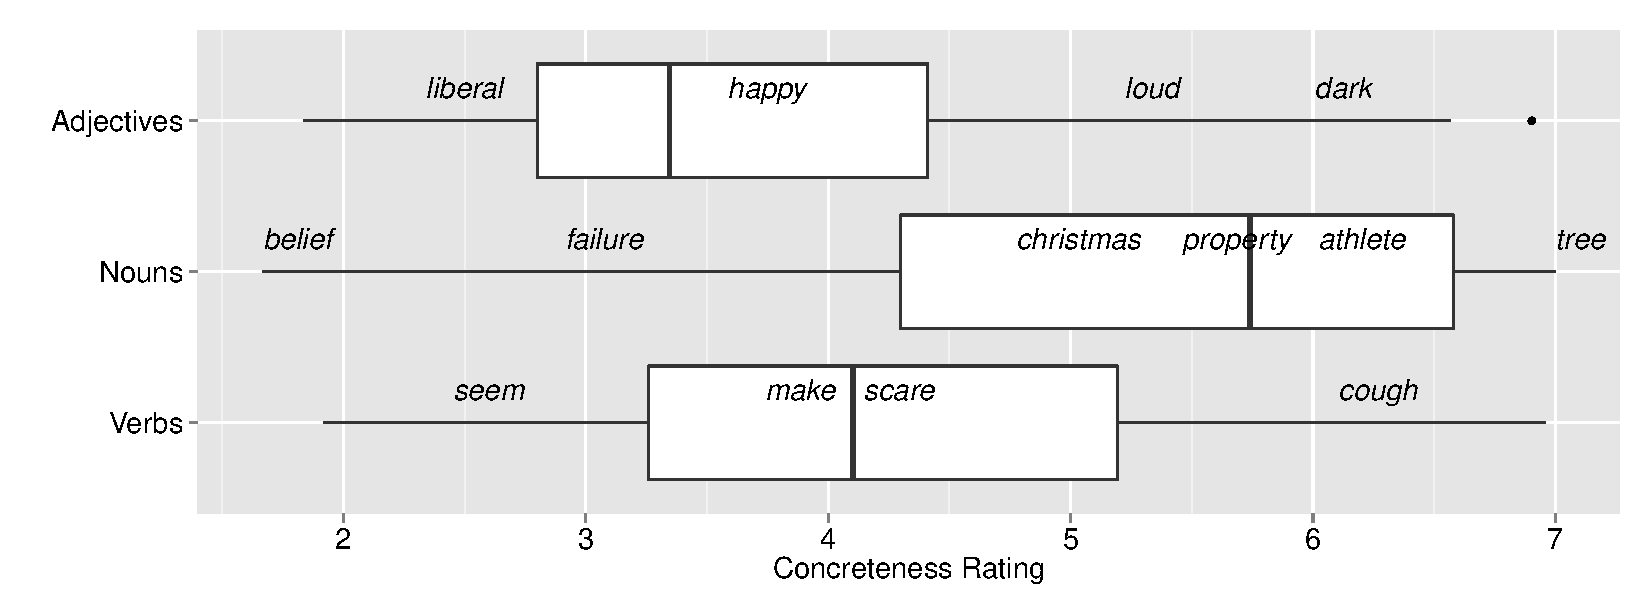
\includegraphics[width = \textwidth]{Chapter_2/Figure_1_CL}  \caption{\label{fig1} Boxplots showing the interaction between concreteness and POS for concepts in USF. The white boxes range from the first to third quartiles and the central vertical line indicates the median.}\end{figure*}  

Unlike the POS distinction, concreteness  is generally considered to be a gradual phenomenon. One benefit of sampling pairs for SimLex-999 from the USF dataset is that most items have been rated according to concreteness on a scale of 1-7 by at least 10 human subjects. As Figure~\ref{fig1} demonstrates, concreteness (as the average over these ratings) interacts with POS on these concepts: nouns are on average more concrete than verbs which are more concrete than adjectives. However, there is also clear variation in concreteness within each POS category. I therefore aimed to select pairs for SimLex-999 that spanned the full abstract-concrete continuum within each POS category. 

After excluding any pairs that contained an item with no concreteness rating, for each potential SimLex-999 pair I considered both the concreteness of the first item and the additive difference in concreteness between the two items. This enabled the sampling to be stratified equally across four classes: (\( C_1\)) concrete first item (rating \(> 4\)) with below-median concreteness difference, (\( C_2\)) concrete first item (rating\( > 4\)), second item of lower concreteness and the difference being greater than the median, (\( C_3\)) abstract first item (rating \( \leq 4\)) with below-median concreteness difference, and (\( C_4\)) abstract first item (rating \(\leq 4\)) with the second item of greater concreteness and the difference being greater than the median. 

\paragraph{Final sampling} From the associated (USF) cohort of potential pairs I selected 600 noun pairs, 200 verb pairs and 100 adjective pairs, and from the unassociated (non-USF) cohort, I sampled 66 nouns pairs, 22 verb pairs and 11 adjective pairs. In both cases, the sampling was stratified such that, in each POS subset, each of the four concreteness classes \(C_1 - C_4\) was equally represented. 

\subsection{Question Design}

The annotator instructions for SimLex-999 are shown in Figure~\ref{fig2}. I did not attempt to formalise the notion of similarity, but rather introduce it via the well-understood idea of synonymy, and in contrast to association. Even if a formal characterisation of similarity existed, the evidence in Section~\ref{motivation} suggests that the instructions would need separate cases to cover different concept types, increasing the difficulty of the rating task. Therefore I preferred to appeal to intuition on similarity, and to verify post-hoc that subjects were able to interpret and apply the informal characterization consistently for each concept type. 

\begin{figure*}[ht]  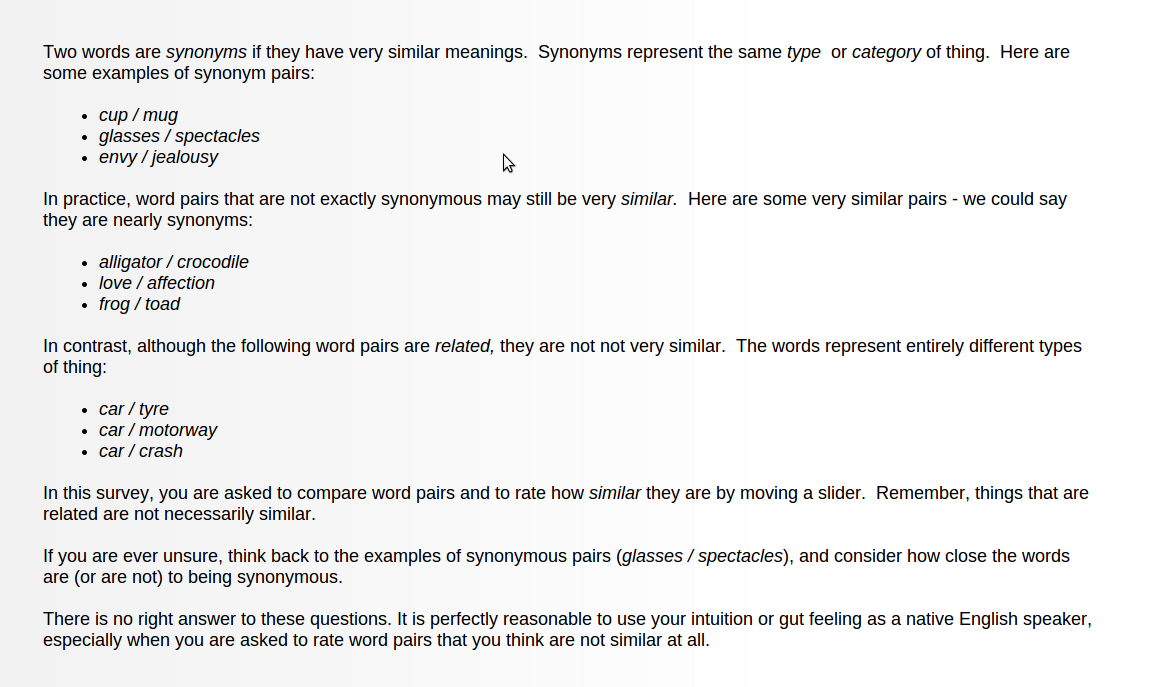
\includegraphics[width = \textwidth]{Chapter_2/screenshot1_CL}  \caption{\label{fig2} Instructions for SimLex-999 annotators.}\end{figure*} 

Immediately following the instructions in Figure~\ref{fig2}, participants were presented with two `checkpoint' questions, one with abstract examples and one with concrete examples. In each case the participant was required to identify the \emph{most similar} pair from a set of three options, all of which were associated, but only one of which was clearly similar (e.g. [\emph{bread, butter}] [\emph{bread, toast}] [\emph{stale, bread}]). After this, the participants began rating pairs in groups of 6 or 7 pairs by moving a slider, as shown in Figure~\ref{fig3}.

This group size was chosen because the (relative) rating of a set of pairs implicitly requires pairwise comparisons between all pairs in that set. Therefore, using larger groups would have increased the cognitive load on the annotators exponentially. Another advantage of grouping was the clear break (submitting a set of ratings and moving to the next page) between the tasks of rating adjective, noun and verb pairs. For better inter-group calibration, from the second group onwards the last pair of the previous group became the first pair of the present group, and participants were asked to re-assign the rating previously attributed to the first pair before rating the remaining new items.  

\begin{figure*}[ht]  


    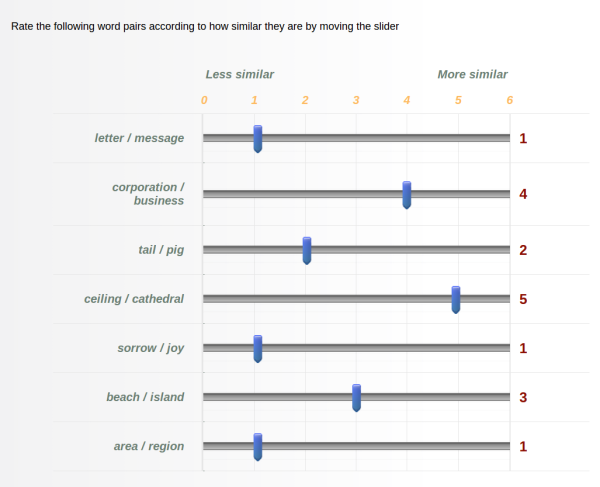
\includegraphics[height=10cm]{Chapter_2/screenshot2_CL}

  \caption{\label{fig3} A group of noun pairs to be rated by moving the sliders. The rating slider was initially at position 0, and it was possible to attribute a rating of 0, although it was necessary to have clicked on the slider in the zero position to assign that rating and proceed to the next page.}

\end{figure*} 

%\begin{figure*}[ht]  \includegraphics[width = 0.5\textwidth]{screenshot2}  \caption{A group of noun pairs to be rated by moving the sliders. }\end{figure*}  


\vspace{2cm}
\subsection{Context-free rating}

As with MEN, WS-353 and RG, SimLex-999 consists of pairs of concept words together with a numerical rating. Thus, unlike in the small evaluation constructed by \cite{huang2012improving}, words are not rated in a phrasal or sentential context. Such meaning-in-context evaluations are motivated by a desire to disambiguate words that otherwise might be considered to have multiple senses.

I did not attempt to construct an evaluation based on meaning-in-context for several reasons. First, determining the set of senses for a given word, and then the set of contexts that represent those senses, introduces a high degree of subjectivity into the design process. Second, ensuring that a model has learned a high quality representation of a given concept would have required evaluating that concept in each of its given contexts, necessitating many more cases and a far greater annotation effort. Third, in the (infrequent) case that some concept \(c_1\) in an evaluation pair \((c_1,c_2)\) is genuinely (etymologically) polysemous, \( c_2 \) can provide sufficient context to disambiguate \(c_1\).\footnote{This is supported by the fact that the WordNet-based methods that perform best at modeling human ratings  model the similarity between concepts \( c_1 \) and \( c_2 \) as the minimum of all pairwise distances between the senses of \(c_1\) and the senses of \(c_2\) \citep{resnik1995using,pedersen2004wordnet}.} Finally, the POS grouping of pairs in the survey can also serve to disambiguate in the case that the conflicting senses of the polysemous concept are of differing POS category.

\subsection{Questionnaire structure}

Each participant was asked to rate 20 groups of pairs on a 0-6 scale of integers (non-integral ratings were not possible). Checkpoint multiple-choice questions were inserted at points between the 20 groups in order to ensure the participant had retained the correct notion of similarity. In addition to the checkpoint of three noun pairs presented before the first group (which contained noun pairs), checkpoint questions containing adjective pairs were inserted before the first adjective group and checkpoints of three verb pairs were inserted before the first verb group.     

From the 999 evaluation pairs, 14 noun pairs, 4 verb pairs and 2 adjective pairs were selected as a \emph{consistency set}. The dataset of pairs was then partitioned into 10 tranches, each consisting of 119 pairs, of which 20 were from the consistency set and the remaining 99 unique to that tranche. To reduce workload, each annotator was asked to rate the pairs in a single tranche only. The tranche itself was divided into 20 groups, with each group corresponding to a single page on the web survey and consisting of 7 pairs (with the exception of the last group of the 20, which had 6). Of the 7 pairs in each group, the first pair was the last pair from the previous group, and the second pair was taken from the consistency set. The remaining pairs were unique to that particular group and tranche. The design enabled control for possible systematic differences between annotators and tranches, which could be detected by variation on the consistency set. 

\subsection{Participants}

500 residents of the USA were recruited from Mechanical Turk, each with at least 95\% approval rate for previous work. Each participant was required to check a box confirming that he or she was a native speaker of English and warned that work would be rejected if the pattern of responses indicated otherwise. The participants were distributed evenly to rate pairs in one of the ten question tranches, so that each pair was rated by approximately 50 subjects. Participants took between 8 and 21 minutes to rate the 119 pairs across the 20 groups, together with the checkpoint questions. 

\subsection{Post-processing}

In order to correct for systematic differences in the overall calibration of the rating scale between respondents, I measured the average (mean) response of each rater on the consistency set. For 32 respondents, the absolute difference between this average and the mean of all such averages was greater than one (though never greater than two); i.e. 32 respondents demonstrated a clear tendency to rate pairs as either more or less similar than the overall rater population. To correct for this bias, I increased (or decreased) the rating of such respondents for each pair by one, except in cases where they had given the maximum rating, six (or minimum rating, zero). This adjustment, which ensured that the average response of each participant was within one of the mean of all respondents on the consistency set, resulted in a small increase to the inter-rater agreement on the dataset as a whole.     

After controlling for systematic calibration differences, I imposed three conditions for the responses of a rater to be included in the final data collation.  First, the average pairwise Spearman correlation of responses with all other responses for a participant could not be more than one standard deviation below the mean of all such averages. Second, the increase in inter-rater agreement when a rater was excluded from the analysis needed to be smaller than at least 50 other raters (i.e. 10\% of raters were excluded on this criterion). Third, I excluded the 6 participants who got one or more of the checkpoint questions wrong. A total of 99 participants were excluded based on one or more of these conditions, but no more than 16 from any one tranche (so that each pair in the final dataset was rated by a minimum of 34 raters). Finally, I computed average (mean) scores for each pair, and transformed all scores linearly from the interval \([0,6]\) to the interval \([0,10]\).

\section{Analysis of Dataset}
\label{analysis}
In this section I analyse the responses of the SimLex-999 annotators and the resulting ratings. First, by considering inter-annotator agreement I examine the consistency with which annotators were able to apply the characterization of similarity outlined in the instructions to the range of concept types in SimLex-999. Second, I verify that a valid notion of similarity was understood by the annotators, in that they were able to accurately separate similarity from association. 

\subsection{Inter-annotator agreement}

\begin{figure*}[ht]  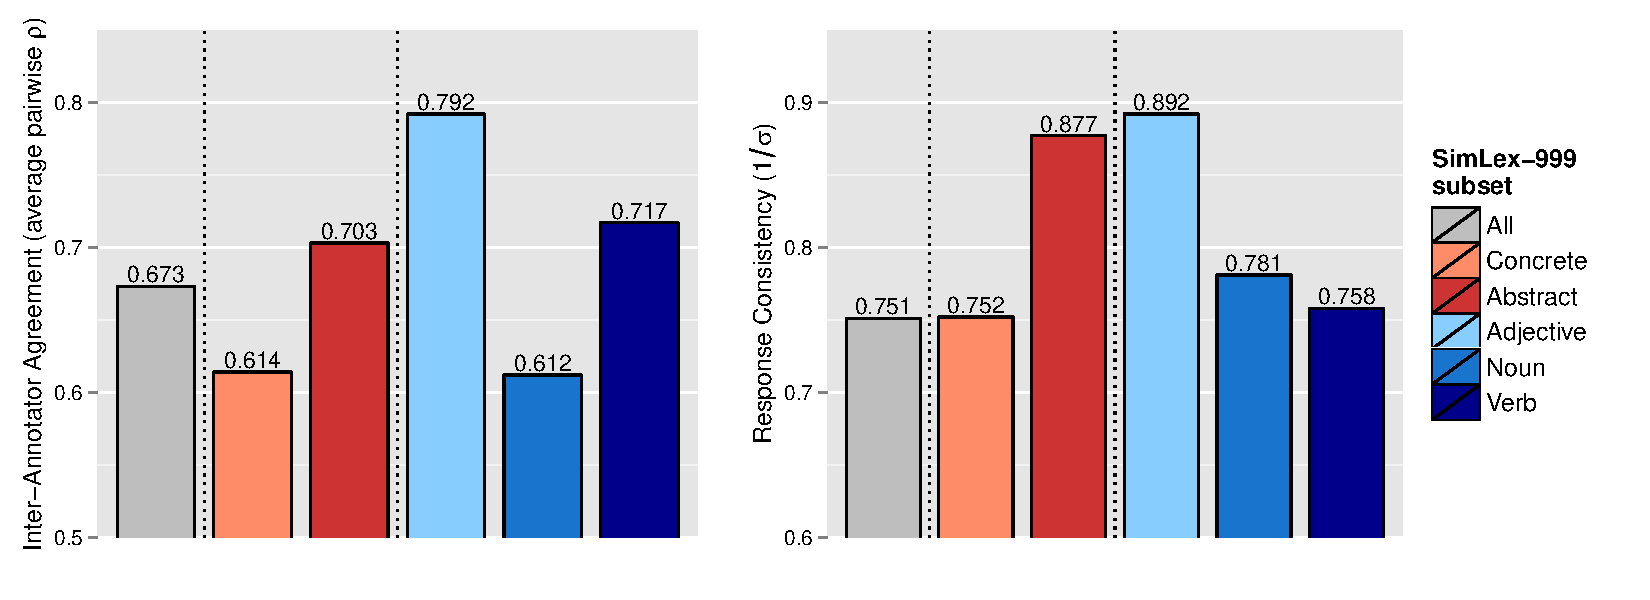
\includegraphics[width = \textwidth]{Chapter_2/Figure_1A_CL}  \caption{\label{fig4} {\bf Left:} Inter-annotator agreement, measured by average pairwise Spearman \(\rho\) correlation, for ratings of concept types in SimLex-999. {\bf Right:} Response consistency, reflecting the standard deviation of annotator ratings for each pair, averaged over all pairs in the concept category.}\end{figure*}  

As in previous annotation or data collection for computational semantics \citep{pado2007flexible,reisinger2010mixture,silberer2014learning} I computed the inter-rater agreement as the average of pairwise Spearman \(\rho\) correlations between the ratings of all respondents. Overall agreement was \(\rho=0.67\). This compares favourably with the agreement on WS-353 (\(\rho=0.61\) using the same method). The design of the MEN rating system precludes a conventional calculation of inter-rater agreement \citep{bruni2012distributional2}. However, two of the creators of MEN who independently rated the dataset achieved an agreement of \(\rho=0.68\).\footnote{Reported at http://clic.cimec.unitn.it/~elia.bruni/MEN. It is reasonable to assume that actual agreement on MEN may be somewhat lower than 0.68 given the small sample size and the expertise of the raters.} 

The SimLex-999 inter-rater agreement suggests that participants were able to understand the (single) characterization of similarity presented in the instructions and to apply it to concepts of various types consistently. This conclusion was supported by inspection of the brief feedback offered by the majority of annotators in a final text field in the questionnaire: 78\% expressed sentiment that the test was clear, easy to complete or some similar sentiment.

Interestingly, as shown in Figure~\ref{fig4} (left), agreement was not uniform across the concept types. Contrary to what might be expected given established concreteness effects \citep{paivio1991dual}, I observed not only higher inter-rater agreement but also less per-pair variability for abstract rather than concrete concepts\footnote{Per-pair variability was measured by calculating the standard deviation of responses for each pair, and averaging these scores across the pairs of each concept type.}. 

Strikingly, the highest inter-rater consistency and lowest per-pair variation (defined as the inverse of the standard deviation of all ratings for that pair) was observed on adjective pairs. While the cause of this effect is not obvious, a possible cause is that many pairs of adjectives in SimLex-999 cohabit a single salient, one-dimensional scale (\emph{freezing > cold > warm > hot}). This may be a consequence of the fact that many pairs in SimLex-999 were selected (from USF) to have a degree of association. On inspection, pairs of nouns and verbs in SimLex-999 do not appear to occupy scales in the same way, possibly since concepts of these POS categories come to be associated via a more diverse range of relations. It seems plausible that humans are able to estimate the similarity of scale-based concepts more consistently than pairs of concepts related in a less uni-dimensional fashion. 

Regardless of cause, however, the high agreement on adjectives is a satisfactory property of SimLex-999. Adjectives exhibit various aspects of lexical semantics that have proved challenging for computational models, including antonymy, polarity \citep{williams2009predicting} and sentiment \citep{wiebe2000learning}. To approach the high level of human confidence on the adjective pairs in SimLex-999, it may be necessary to focus particularly on developing automatic ways to capture these phenomena. 

\subsection{Response validity: Similarity not association}	



Inspection of the SimLex-999 ratings indicated that pairs were indeed evaluated according to similarity rather than association. Table~\ref{tab2} includes examples that demonstrate a clear dissociation between the two semantic relations. 



 \begin{table}[t]\begin{center}\begin{tabular}{l|l|c|r|r|r|r}





C1 & C2 & POS & USF* & USF rank \scriptsize{/999} & SimLex & SimLex rank \scriptsize{/999} \\



\hline \emph{dirty} & \emph{narrow} & A & 0.00 & 999 & 0.30 & 996 \\



\emph{student} & \emph{pupil} & N & 6.80 & 12 & 9.40 & 12 \\

\emph{win} & \emph{dominate} & V & 0.41 & 364 & 5.68 & 361 \\



\hdashline \emph{smart} & \emph{dumb} & A & 2.10 & 92 & 0.60 & 947 \\

\emph{attention} & \emph{awareness} & N &  0.10 & 895 & 8.73 & 58 \\

\emph{leave} & \emph{enter} & V & 2.16 & 89 & 1.38 & 841 \\
\end{tabular}
\end{center}\caption{\label{tab2} {\bf Top:  Similarity aligns with association} Pairs with a small difference in rank between USF (association) and SimLex-999 (similarity) scores for each POS category. {\bf Bottom: Similarity contrasts with association} Pairs with a high difference in rank for each POS category. *Note that the distribution of USF association scores on the interval [0,10] is highly skewed towards the lower bound in both SimLex-999 and the USF dataset as a whole.}\end{table}

\begin{figure*}[ht]  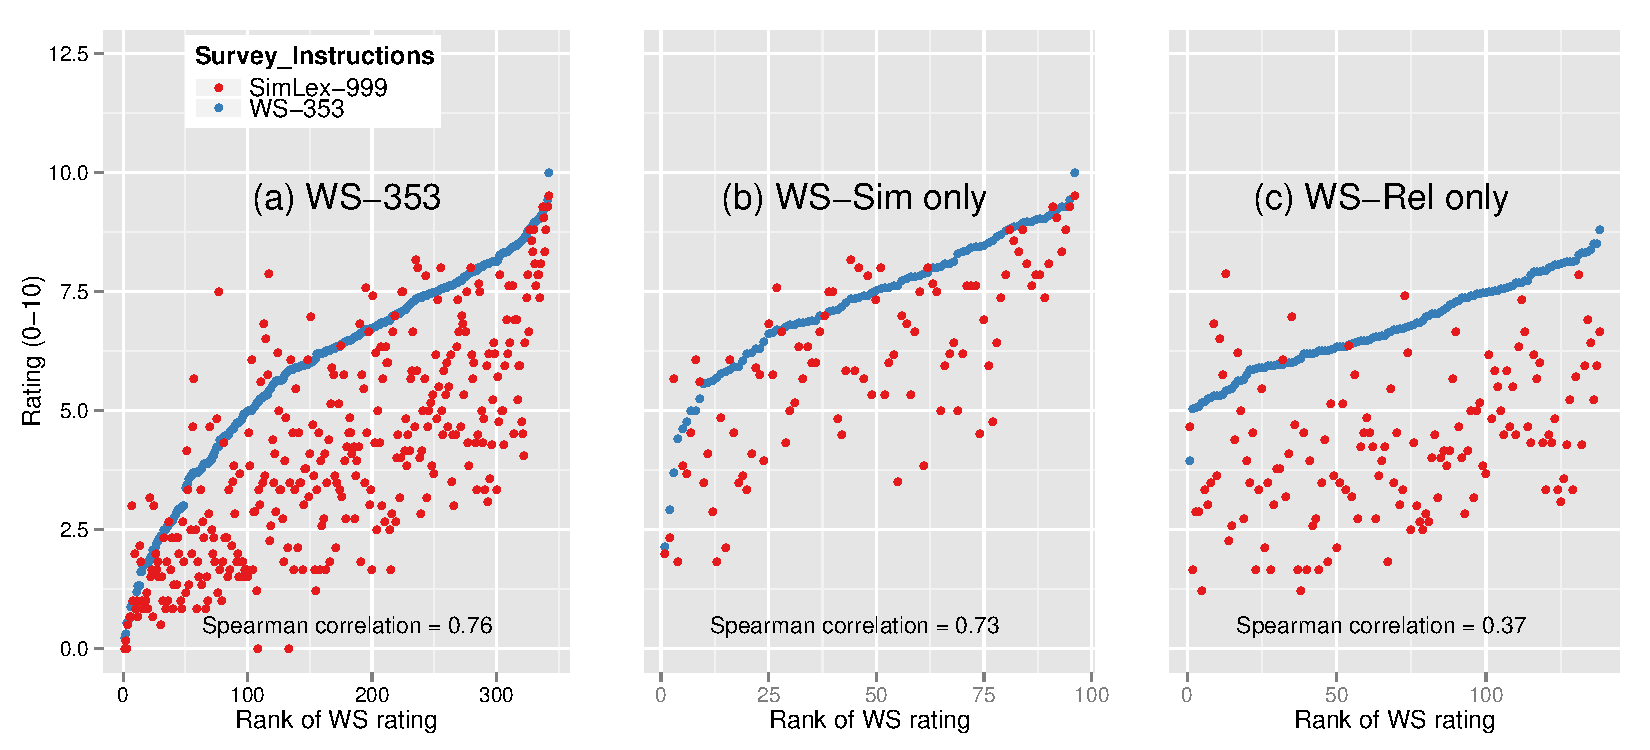
\includegraphics[width =\textwidth]{Chapter_2/Figure_6_CL} \caption{\label{fig5} {\bf(a)} Pairs rated by WS-353 annotators (blue points, ranked by rating) and the corresponding rating of annotators following the SimLex-999 instructions (red points). {\bf(b-c)} The same analysis, restricted to pairs in the WS-Sim or WS-Rel subsets of WS-353.}\end{figure*}  



To verify this effect quantitatively, I recruited 100 additional participants to rate the WS-353 pairs, but following the SimLex-999 instructions and question format. As shown in Fig 5(a), there were clear differences between these new ratings and the original WS-353 ratings. In particular, a high proportion of pairs was given a lower rating by subjects following the SimLex-999 instructions than those following the WS-353 guidelines: The mean SimLex rating was 4.07 compared with 5.91 for WS-353. 



This was consistent with the expectations that pairs of associated but dissimilar concepts would receive lower ratings based on the SimLex-999 than on the WS-353 instructions while pairs that were both associated and similar would receive similar ratings in both cases. To confirm this, I compared the WS-353 and SimLex-999-based ratings on the subsets WS-Rel and WS-Sim, which were hand-sorted by \cite{agirre2009study} to include pairs connected by association (and not similarity) and those connected by similarity (but possibly also association) respectively.  



As shown in Figure~\ref{fig5}(b-c), the correlation between the SimLex-999-based and WS-353 ratings was notably higher (\(\rho=0.73\)) on the WS-Sim subset than the WS-Rel subset (\(\rho=0.38\)). Specifically, the tendency of subjects following the SimLex-999 instructions to assign lower ratings than those following the WS-353 instructions was far more pronounced for pairs in WS-Sim (Figure~\ref{fig5}(b)) than for those in WS-Rel (\ref{fig5}(c)). This observation suggest that the associated but dissimilar pairs in WS-353 were an important driver of the overall lower mean for SimLex-999-based ratings, and thus provide strong evidence that the SimLex-999 instructions do indeed enable subjects to distinguish similarity from association effectively. 


\subsection{Finer-grained Semantic Relations}

I have established the validity of similarity as a notion understood by human raters and distinct from association. However, much theoretical semantics focuses on relations between words or concepts that are finer-grained than similarity and association. These include \emph{meronymy} (a part to its whole, e.g. \emph{blade - knife}), \emph{hypernymy} (a category concept to a member of that category, e.g. \emph{animal - dog}) and \emph{cohyponymy} (two members of the same implicit category, e.g. the pair of animals \emph{dog - cat}) \citep{cruse1986lexical}. Beyond theoretical interest, these relations can have practical relevance. For instance, hypernymy can form the basis of semantic entailment and therefore textual inference: the proposition \emph{a cat is on the table} entails that \emph{an animal is on the table} precisely because of the hypernymy relation from animal to cat. 

I chose not to make these finer-grained relations the basis of the evaluation for several reasons. At present, detecting relations such as hypernymy using distributional methods is challenging, even when supported by supervised classifiers with access to labelled pairs \citep{levy2015supervised}. Such a designation can seem to require specific world-knowledge (is a \emph{snake} a \emph{reptile}?), can be gradual, as evidenced by typicality effects \citep{rosch1976structural}, or simply highly subjective. Moreover, a fine-grained relation \(R\) will only be attested (to any degree) between a small subset of all possible word pairs, whereas similarity can in theory be quantified for any two words chosen at random. I thus considered a focus on fine-grained semantic relations to be less appropriate for a general-purpose evaluation of representation quality.  

Nevertheless, post-hoc analysis of the SimLex annotator responses and fine-grained relation classes, as defined by lexicographers, yields further interesting insights into the nature of both similarity and association. Of the 999 word pairs in SimLex, 382 are also connected by one of the common finer-grained semantic relations in WordNet. For each of these relations, Figure~\ref{fig6} shows the average similarity rating and average USF free association score for all pairs that exhibit that relation. 

In cases where a relationship of hypernymy/hyponymy exists between the words in a pair (not necessarily immediate - \(1\_hypernym, 2\_hypernym\) etc.) similarity and association coincide. Hyper/hyponym pairs that are separated by fewer levels in the WordNet hierarchy are both more strongly associated and rated as more similar. However, there are also interesting discrepancies between similarity and association. Unsurprisingly, pairs that are classed as synonyms in WordNet (i.e. having at least one sense in some common synset) are rated as more similar than pairs of any other relation type by SimLex annotators. In contrast, antonyms are the most strongly-associated word pairs among these finer-grained relations. Further, pairs consisting of a meronym and holonym (part and whole) are comparatively strongly associated but not judged to be similar. 

The analysis also highlights a case that can be particularly problematic when rating similarity;  cohyponyms, or members of the same salient category (such as \emph{knife} and \emph{fork}). I gave no specific guidelines for how to rate such pairs in the SimLex annotator instructions, and whether they are considered similar or not seems to be a matter of perspective. On one hand, their membership of a common category could make them appear similar, particularly if the category is relatively specific. On the other hand, in the case of \emph{knife} and \emph{fork}, for instance, the underlying category \emph{cutlery} might provide a backdrop against which the differences of distinct members become particularly salient. 

\begin{figure}[ht]  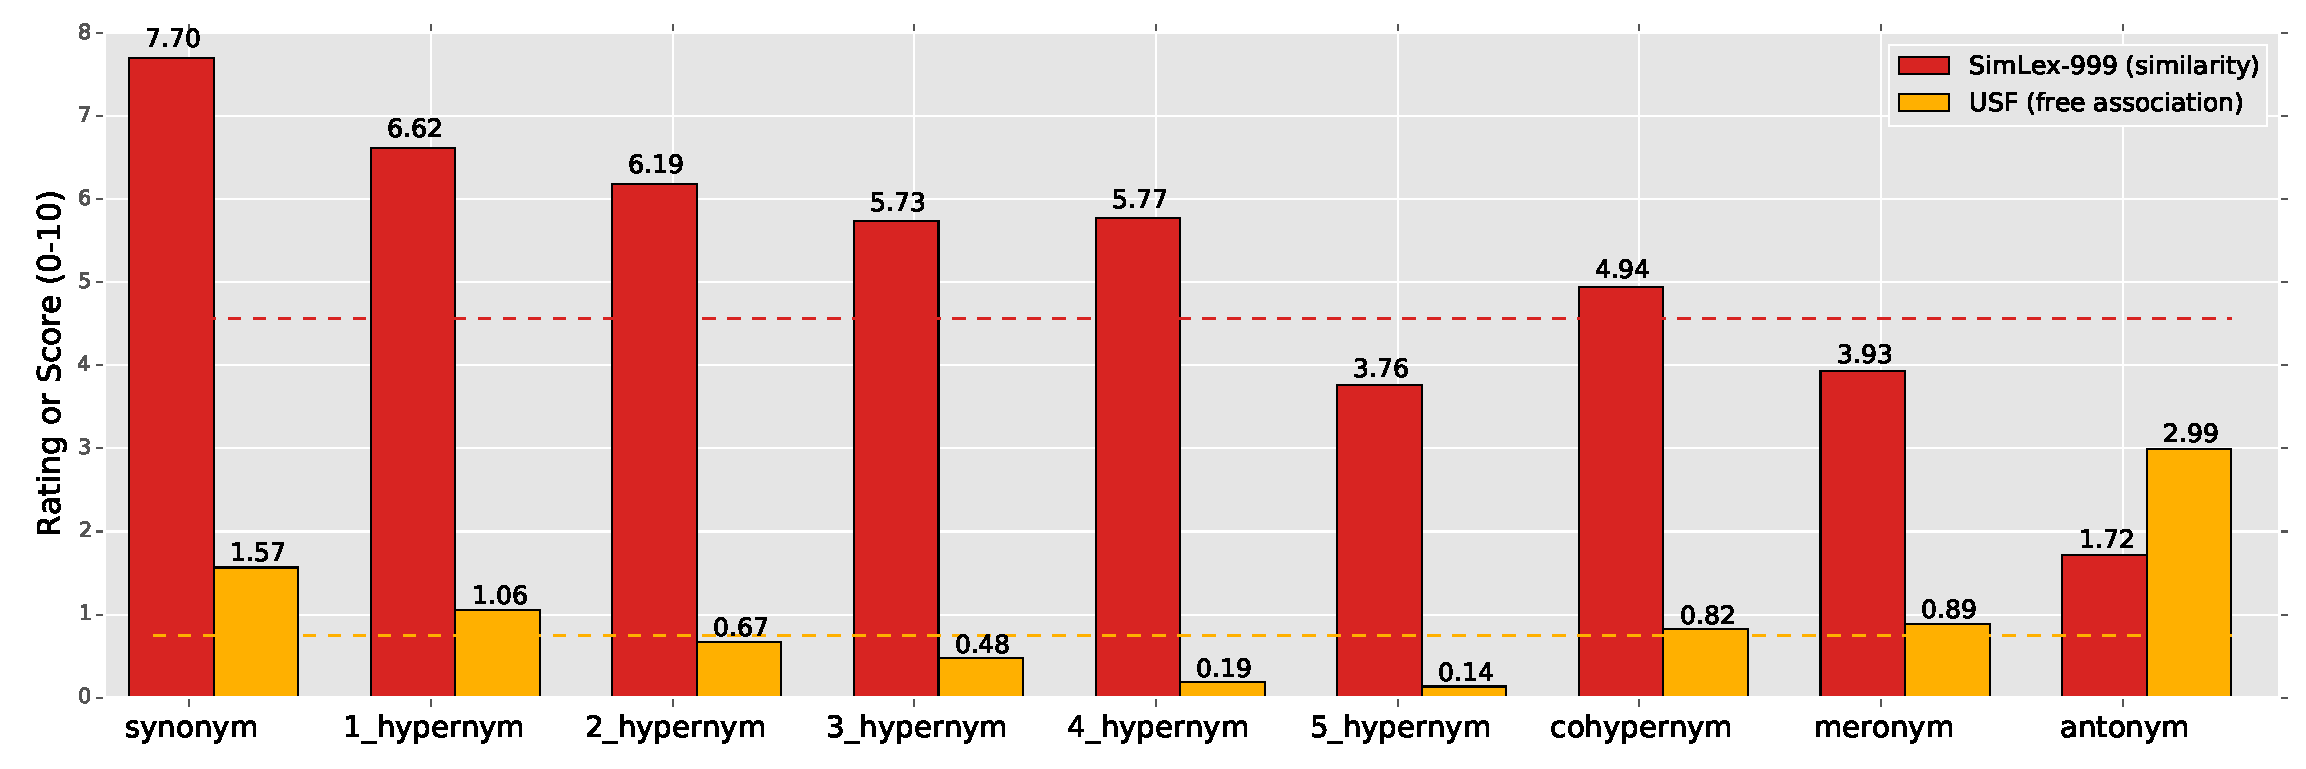
\includegraphics[width =\textwidth]{Chapter_2/simlex_relations_CL}  \caption{\label{fig6} Average SimLex and USF free association scores across pairs representing different fine-grained semantic relations. All relations were extracted from WordNet. \(n\_hypernym\) refers to a direct hypernymy path of length \(n\). Note that the average SimLex rating across all 999 word pairs (dashed red line) is much higher than the average USF rating (dashed golden line) because of differences in the rating procedure. The more interesting differences concern the relative strength of similarity vs. association across the different relation types.}\end{figure}  

\section{Evaluating Models with SimLex-999}
\label{evaluation}

In this section, I demonstrate the applicability of SimLex-999 by analysing the performance of various distributional semantic models in estimating the new ratings. The models were selected to cover the main classes of representation learning architectures \citep{baroni2014don}: vector space co-occurrence (counting) models and neural language models (NLM)s \citep{Bengio2003lm}. I first show that SimLex-999 is in general notably more difficult for models to estimate than existing gold standards. I then conduct more focused analyses on the various concept subsets defined in SimLex-999, exploring possible causes for the comparatively low performance of current models and, in turn, demonstrating how SimLex-999 can be applied to investigate such questions.    

\subsection{Neural language models for word representation}
\label{prev}

\paragraph{\bf Collobert \& Weston}

\cite{collobert2008unified} apply the architecture of an NLM to learn a word representations \(v_w\) for each word \(w\) in some corpus vocabulary \( V\). Each sentence \( s\) in the input text is represented by a matrix containing the vector representations of the words in \(s\) in order. The model then computes output scores \(f(s) \) and \(f(s^w) \), where \(s^w\) denotes an `incorrect' sentence created from \(s\) by replacing its last word with some other word \( w\) from \(V\). Training involves updating the parameters of the function \(f\) and the entries of the vector representations \(v_w\) such that  \(f(s)\) is larger than \(f(s^w) \) for any \(w\) in \(V\), other than the correct final word of \(s\). This corresponds to minimising the sum of the following sentence objectives \( C_s\) over all sentences in the input corpus, which is achieved via (mini-batch) stochastic gradient descent:

\[ C_{s}  = \sum_{w \in V} max(0,1-f(s) + f(s^w)). \]

The relatively low-dimension, dense (vector) representations learned by this model and the other NLMs introduced in this section are sometimes referred to as \emph{embeddings} \citep{turian2010word}. \cite{collobert2008unified} train their models on 852 million words of text from a 2007 dump of Wikipedia and the RCV1 Corpus \citep{lewis2004rcv1} and use their embeddings to achieve state-of-the-art results on a variety of NLP tasks. I downloaded the embeddings directly from the authors' webpage.\footnote{http://ml.nec-labs.com/senna/}

 \paragraph{\bf Huang et al.}

\cite{huang2012improving} present a NLM that learns word embeddings to maximise the likelihood of predicting the last word in a sentence \(s\) based on (i) the previous words in that sentence (local context - as with \cite{collobert2008unified}) and (ii) the document \( d\) in which that word occurs (global context). As with \cite{collobert2008unified}, the model represents input sentences as a matrix of word embeddings. In addition, it represents documents in the input corpus as single-vector averages over all word embeddings in that document. It can then compute scores \(g(s,d )\) and \(g(s^w, d) \), where as before \(s^w\) is a sentence with an `incorrect' randomly-selected last word. Training is again by stochastic gradient descent, and corresponds to minimising the sum of the sentence objectives \(C_{s,d} \) over all of the sentences in the corpus:

\[ C_{s,d}  = \sum_{w \in V} max(0,1-g(s,d) + g(s^w,d)). \]

The combination of local and global contexts in the objective encourages the final word embeddings to reflect aspects of both the meaning of nearby words and of the documents in which those words appear. When learning from 990m words of wikipedia text, Huang et al. report a Spearman correlation of \(\rho = 71.3\) between the cosine similarity of their model embeddings and the WS-353 scores, which constitutes state-of-the-art performance for a NLM model on that dataset. Embeddings were again downloaded from the authors' webpage.\footnote{\url{www.socher.org}.}

\paragraph{\bf Log-linear models}
\label{shallow}
\cite{mikolov2013efficient} propose a framework for learning word embeddings using neural language models that are much shallower than those of standard NLMs. This enables faster representation learning for large vocabularies. Despite this simplification, the resulting embeddings achieve state-of-the-art performance on several semantic tasks including sentence completion and analogy modelling \citep{mikolov2013efficient,mikolov2013distributed}. In fact, ~\cite{mikolov2013efficient} present two related architectures, \emph{Skipgram} and \emph{CBOW}. Their experiments and those carried out since~\citep{baroni2014don} reveal the performance of these two approaches to be similar, so we focus our analyses on the (marginally) simpler variant, Skipgram.    

For each word type \(w\) in the vocabulary \(V\), the Skipgram model learns both a `source-embedding' \( r_{w} \in \mathbb{R}^d\) and a `context-embedding' \(\hat{r}_{w} \in \mathbb{R}^d\) such that, given a source word, its ability to predict nearby context words is maximised. The probability of seeing context word \(c\) given source \(w\) is defined as:  

\[p(c|w)  = \frac{\me^{\hat{r}_{c} \cdot r_{w}}}{\sum_{v \in V} \me^{\hat{r}_v\cdot r_{w}}}.\]

The model learns from a set of (source-word, context-word) pairs, extracted from a corpus of sentences as follows. In a given sentence \(s\) (of length \(N\)), for each position \( n \leq N\), each word \(w_n\) is treated in turn as a source word. An integer \( {t(n)} \) is then sampled from a uniform distribution on \( \{1, \dots k \} \), where \(k > 0\) is a predefined maximum context-window parameter. The pair tokens \( \{(w_n, w_{n+j}): -{t(n)}\leq j \leq {t(n)}, w_i \in s \}\) are then appended to the training data. Thus, source/context training pairs are such that (i) only words within a \(k\)-window of the source are selected as context words for that source, and (ii) words closer to the source are more likely to be selected than those further away.

The training objective is then to maximise the log probability \( T\), across of all such examples from \(s\), and then across all sentences in the corpus:

\[ T = \frac{1}{N} \sum_{n=1}^{N} \sum_{-{t(n)}\leq j \leq {t(n)}, j\neq 0} log(  p(w_{n+j}|w_{n}) ). \]

The CBOW architecture differs from the Skipgram in that, for each position in the corpus, the current word is taken to be the object of prediction (the context), and the source from which it is predicted is the combination (via either average or sum) of words in a surrounding window. Both the CBOW and Skipgram models are optimsed via stochastic gradient descent using a linearly decaying learning rate. 

As with other NLMs, the Skipgram and CBOW models capture conceptual semantics by exploiting the fact that words appearing in similar linguistic contexts are likely to have similar meanings. During training, the model adjusts its embeddings to increase the probability of observing the training corpus. For the Skipgram model, since this probability increases with \(p(c|w)\), and \(p(c|w)\) increases with the dot product \( \hat{r}_c\cdot r_{w} \), the updates have the effect of moving each source embedding incrementally `closer' to the context-embeddings of its collocates. In the source embedding space, this results in embeddings of concept words that regularly occur in similar contexts moving closer together. It is in this way that Skipgram implicitly exploits the Distributional Hypothesis.\footnote{See Section~\ref{conclusion} for more about the connections between NLMs and traditional vector space models.}

I use the author's Word2vec software in order to train their model and use the source embeddings in the evaluations. I experimented with embeddings of dimension 100, 200, 300, 400 and 500 and found that 200 gave the best performance on both WS-353 and SimLex-999. 

\subsection{\bf Vector space (counting) models}

To place the performance of the NLMs in context, I compared their performance with vector space models, following the guidelines for optimal performance outlined by \cite{kiela2014systematic}. After extracting the 2000 most frequent word tokens in the corpus that are not in a common list of stopwords\footnote{Taken from the Python Natural Language Toolkit \citep{bird2006nltk}.} as features, I populated a matrix of co-occurrence counts with a row for each of the concepts in some pair in the evaluation sets, and a column for each of the features. Co-occurrence was counted within a specified window size, although never across a sentence boundary. This resulting matrix was then weighted according to Pointwise Mutual Information (PMI) \citep{recchia2009more}. The rows of the resulting matrix constitute the vector representations of the concepts.   

\paragraph{\bf LSA} As proposed initially by \cite{landauer1997solution}, I also experimented with models in which Singular Value Decomposition (SVD) \citep{golub1970singular} is applied to the PMI-weighted VSM matrix, reducing the dimension of each concept representation to 300 (which yielded best results after experimenting, as before, with 100-500 dimension vectors). 

\vspace{1\baselineskip}

\noindent 
For each model described in this section, similarity was calculated as the cosine similarity between the (vector) representations learned by that model. 

\subsection{Results}

In experimenting with different models on SimLex-999, I aimed to answer the following questions: (i) How well do the established models perform on SimLex-999 versus on existing gold standards? (ii) Are any observed differences caused by the potential of different models to measure similarity vs. association? (iii) Are there interesting differences in ability of models to capture similarity between adjectives vs nouns vs verbs? (iv) In this case, are the observed differences driven by concreteness, and its interaction with POS, or are other factors also relevant?

\paragraph{\bf Overall performance on SimLex-999}
\label{assoc}

\begin{figure*}[ht]  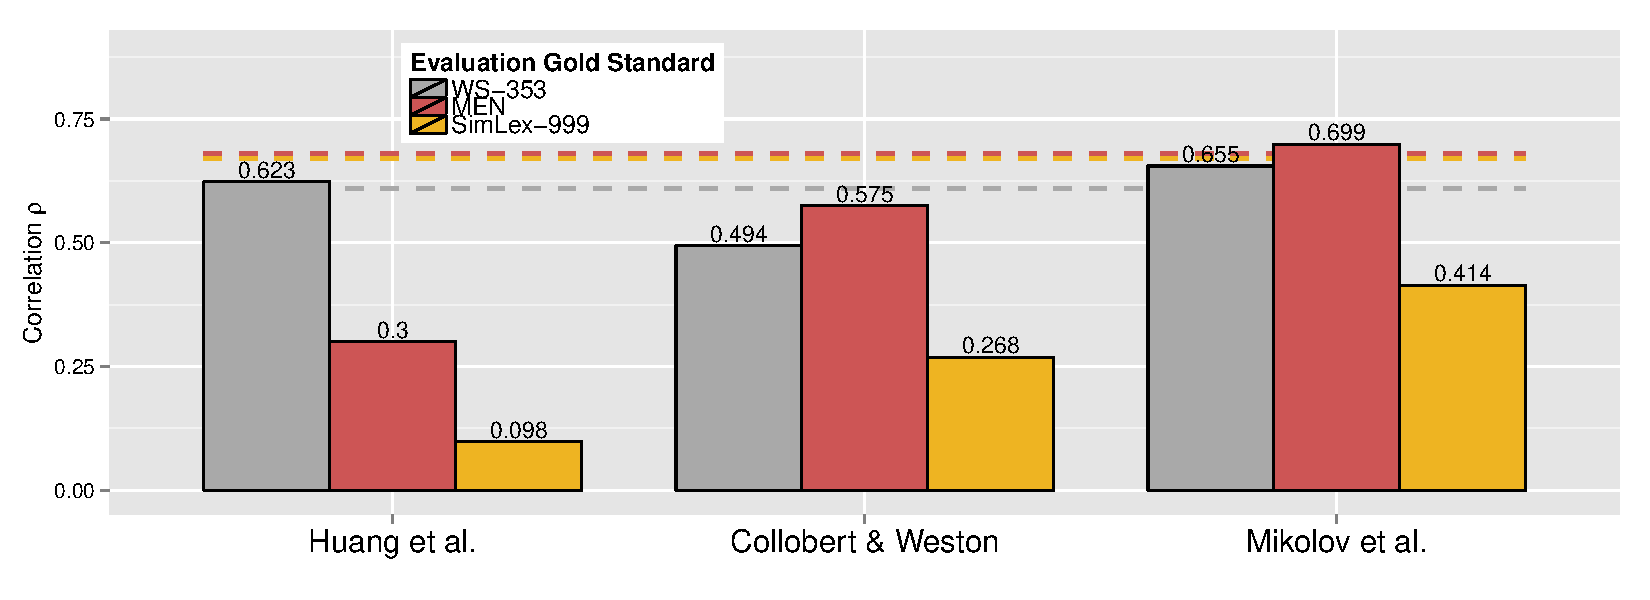
\includegraphics[width = \textwidth, height=5cm]{Chapter_2/Figure_2A_CL} \caption{\label{fig7}Performance of NLMs on WS-353, MEN and SimLex-999. All models are trained on Wikipedia; note that as Wikipedia is constantly growing, the \protect\cite{mikolov2013efficient} model exploited slightly more training data ($\approx$1000m tokens) than the \protect\cite{huang2012improving} model ($\approx$990m), which in turn exploited more than the \protect\cite{collobert2008unified} model ($\approx$852m). Dashed horizontal lines indicate the level of inter-annotator agreement for the three datasets.}\end{figure*}

\begin{figure*}[ht]  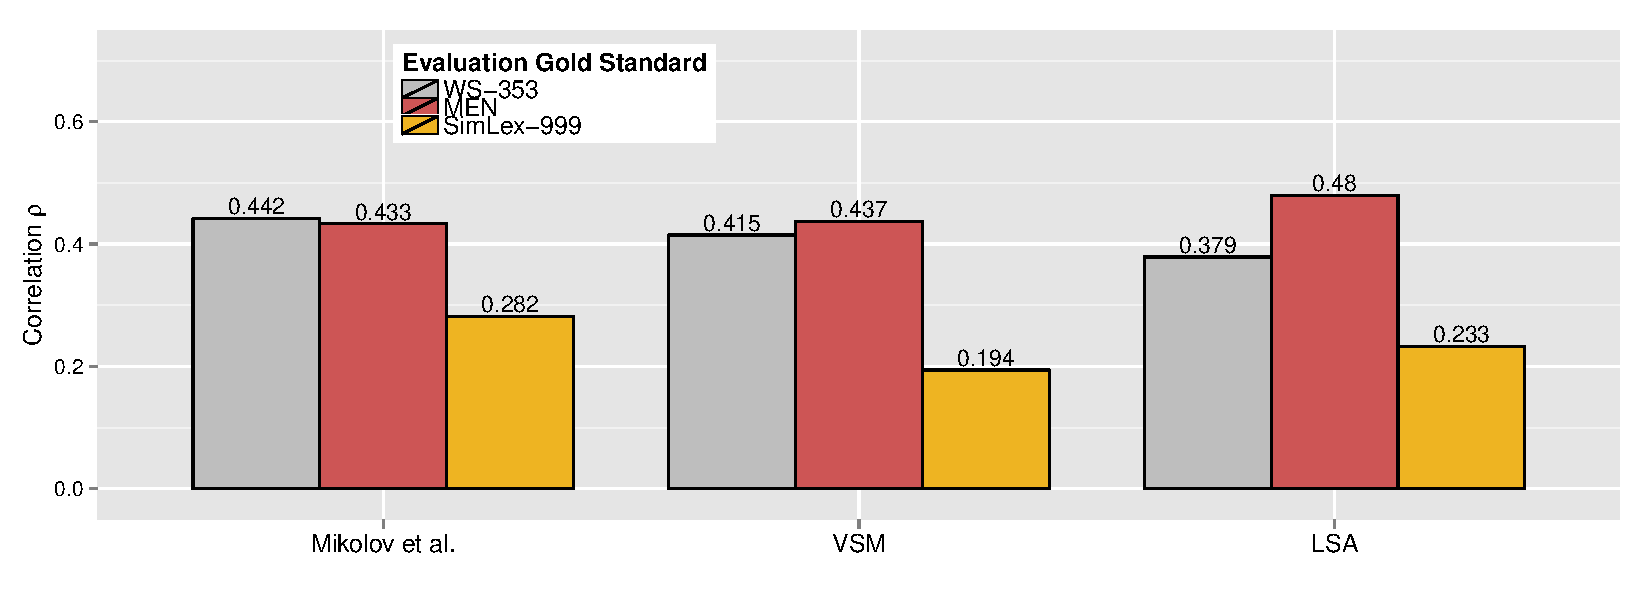
\includegraphics[width = \textwidth,height=5cm]{Chapter_2/Figure_2B_CL}  \caption{\label{fig8}Comparison between the leading NLM, \emph{Mikolov et al.}, the vector space model, \emph{VSM}, and the \emph{LSA} model. All models were trained on the $\approx$150m word RCV1 Corpus \protect\citep{lewis2004rcv1}.}\end{figure*}

Figure~\ref{fig7} shows the performance of the NLMs on SimLex-999 versus on comparable datasets, measured by Spearman's \(\rho\) correlation. All models estimate the ratings of MEN and WS-353 more accurately than SimLex-999. The \cite{huang2012improving} model performs well on WS-353,\footnote{This score, based on embeddings downloaded from the authors' webpage, is notably lower than the score reported by \cite{huang2012improving} mentioned in Section~\ref{prev}.} but is not very robust to changes in evaluation gold standard, and performs worst of all the models on SimLex-999. Given the focus of the WS-353 ratings, it is tempting to explain this by concluding that the global context objective leads the \cite{huang2012improving} model to focus on association rather than similarity. However, the true explanation may be less simple, since the \cite{huang2012improving} model performs weakly on the association-based MEN dataset. The \cite{collobert2008unified} model is more robust across WS-353 and MEN, but still does not match the performance of the \cite{mikolov2013efficient} model on SimLex-999. 

Figure~\ref{fig8} compares the best performing NLM model \citep{mikolov2013efficient} with the VSM and LSA models.\footnote{I conduct this comparison on the smaller RCV1 Corpus \citep{lewis2004rcv1} because training the VSM and LSA models is comparatively slow.}  In contrast to recent results that emphasise the superiority of NLMs over alternatives \citep{baroni2014don}, I observed no clear advantage for the NLM over the VSM or LSA when considering the association-based gold standards WS-353 and MEN together. While the NLM is the strongest performer on WS-353, LSA is the strongest performer on MEN. However, the NLM model performs notably better than the alternatives at modelling similarity, as measured by SimLex-999. 

Comparing all models in Figures~\ref{fig7} and~\ref{fig8} suggests that SimLex-999 is notably more challenging to model than the alternative datasets, with correlation scores ranging from 0.098 to 0.414. Thus, even when state-of-the-art models are trained for several days on massive text corpora,\footnote{Training times reported by \cite{huang2012improving} and by \cite{collobert2008unified} at \url{http://ronan.collobert.com/senna/}.} their performance on SimLex-999 is well below the inter-annotator agreement (Figure~\ref{fig7}). This suggests that there is ample scope for SimLex-999 to guide the development of improved models. 

\paragraph{\bf Modeling similarity vs. association}

The comparatively low performance of NLM, VSM and LSA models on SimLex-999 compared with MEN and WS-353 is consistent with the hypothesis that modelling similarity is more difficult than modelling association. Indeed, given that many strongly-associated but dissimilar pairs, such as [\emph{coffee, cup}], are likely to have high co-occurrence in the training data, and that all models infer connections between concepts from linguistic co-occurrence in some form or another, it seems plausible that models may overestimate the similarity of such pairs because they are `distracted' by association.

To test this hypothesis more precisely, I compared the performance of models on the whole of SimLex-999 versus its 333 most associated pairs (according to the USF free association scores). Importantly, pairs in this strongly-associated subset still span the full range of possible similarity scores (min similarity = 0.23 [\emph{shrink, grow}], max similarity = 9.80 [\emph{vanish, disappear}]).     

As shown in Figure~\ref{fig9}, all models performed worse when the evaluation was restricted to pairs of strongly-associated concepts, which was consistent with the hypothesis. The \cite{collobert2008unified} model was better than the \cite{huang2012improving} model at estimating similarity in the face of high association. This not entirely surprising given the global-context objective in the latter model, which may have encouraged more association-based connections between concepts. The Mikolov et al. model, however, performed notably better than both other NLMs. Moreover, this superiority is proportionally greater when evaluating on the most associated pairs only (as indicated by the difference between the red and grey bars), suggesting that the improvement is driven at least in part by an increased ability to `distinguish' similarity from association. 

\begin{figure*}[]  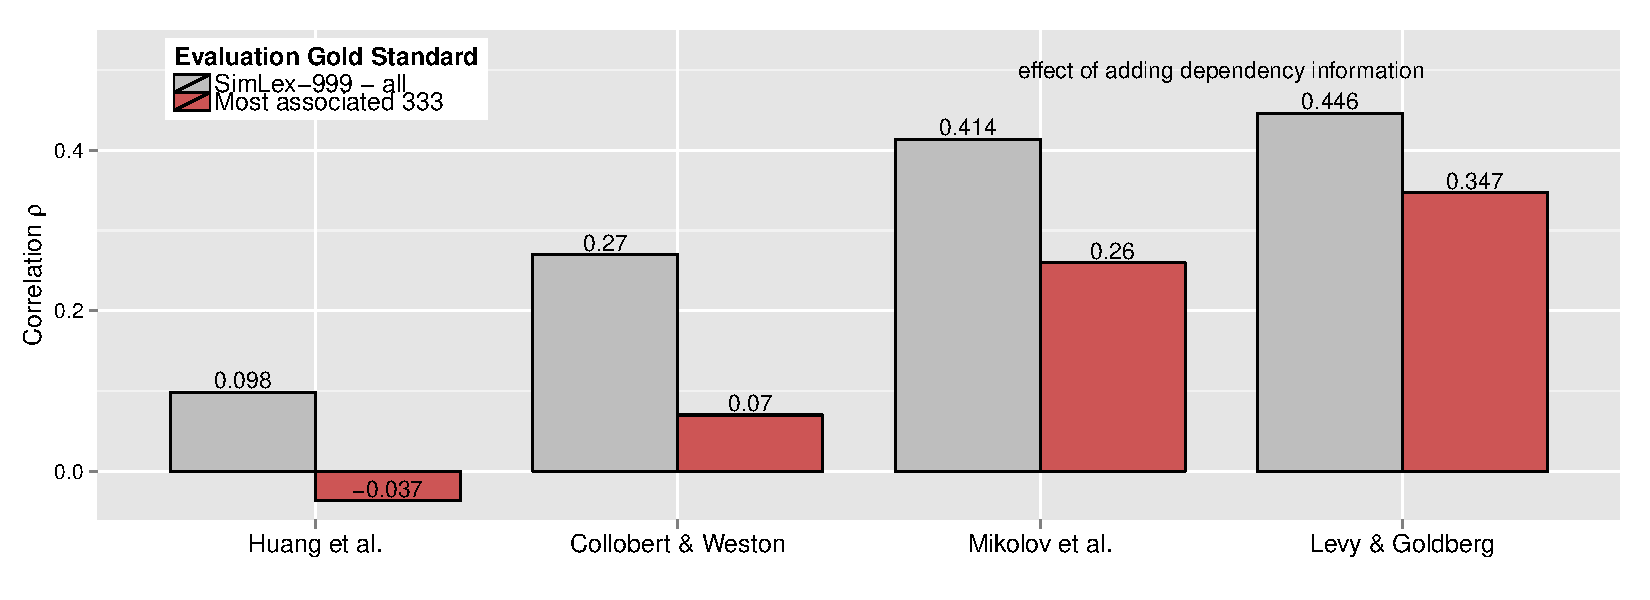
\includegraphics[width = \textwidth,height=5cm]{Chapter_2/Figure_3A_CL}  \caption{\label{fig9} The ability of NLMs to model the similarity of highly-associated concepts versus concepts in general. The two models on the right hand side also demonstrate the effect of training an NLM (the \protect\cite{mikolov2013efficient} model) on running-text (\emph{Mikolov et al.}) vs. on dependency-based input (\emph{Levy \& Goldberg}).}\end{figure*}

In a futher analysis designed to shed light on how distributional models captures information pertinent to similarity, I compared the modification of the Skipgram of \cite{levy2014dependency}, in which source/context pairs are restricted to those in a (syntactic) dependency relationship. It was already suggested by \cite{levy2014dependency} that such a modification could yield a semantic space better ordered to semantic equivalence or similarity, although their demonstration of this effect was somewhat informal 

As illustrated in Figure~\ref{fig9}, the dependency-based embeddings outperform the original (running text) embeddings trained on the same corpus. Moreover, the comparatively large increase in the red bar compared to the grey bar suggests that an important part of the improvement of the dependency-based model derives from a greater ability to discern similarity from association. 

\begin{figure*}[]  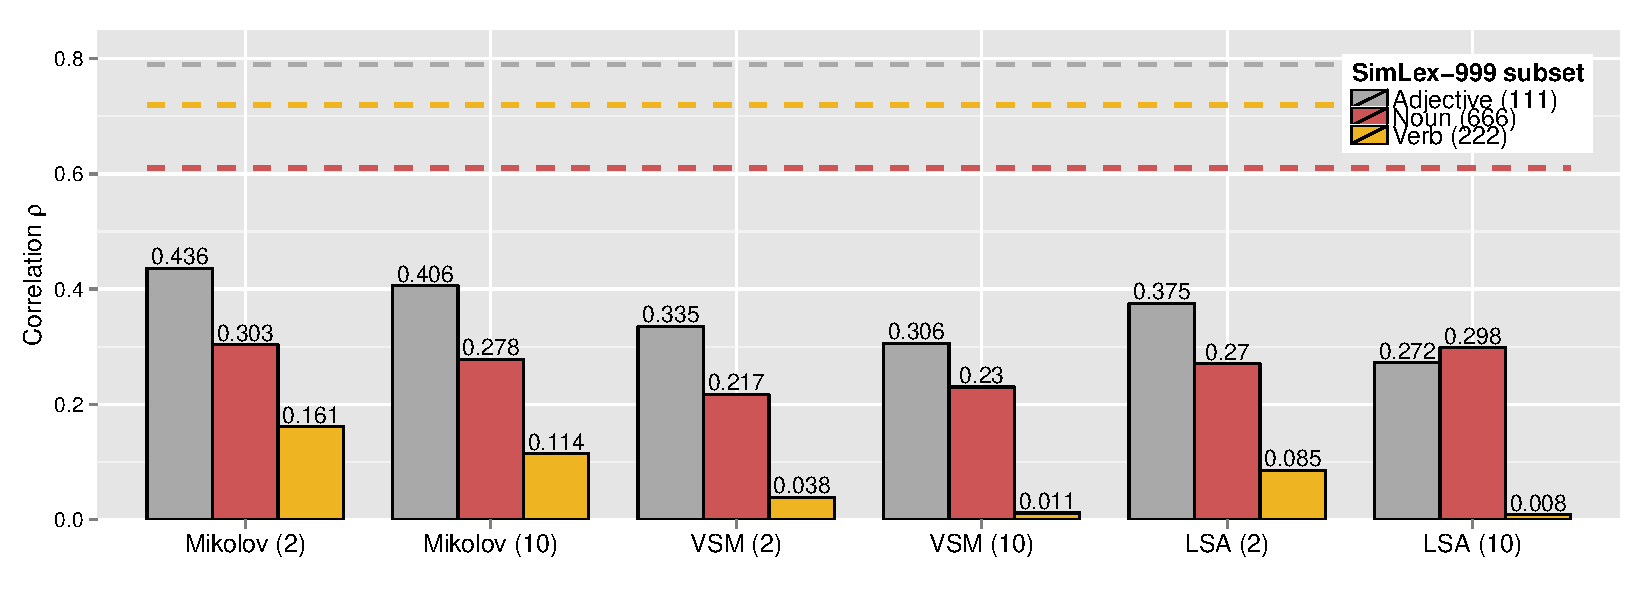
\includegraphics[width = \textwidth,height=5cm]{Chapter_2/Figure_5_CL}  \caption{~\label{fig11} Performance of models on POS-based subsets of SimLex-999. The window size for each model is indicated in parentheses. Inter-annotator agreement for each POS is indicated by the dashed horizontal line.}\end{figure*}

\begin{figure}[]  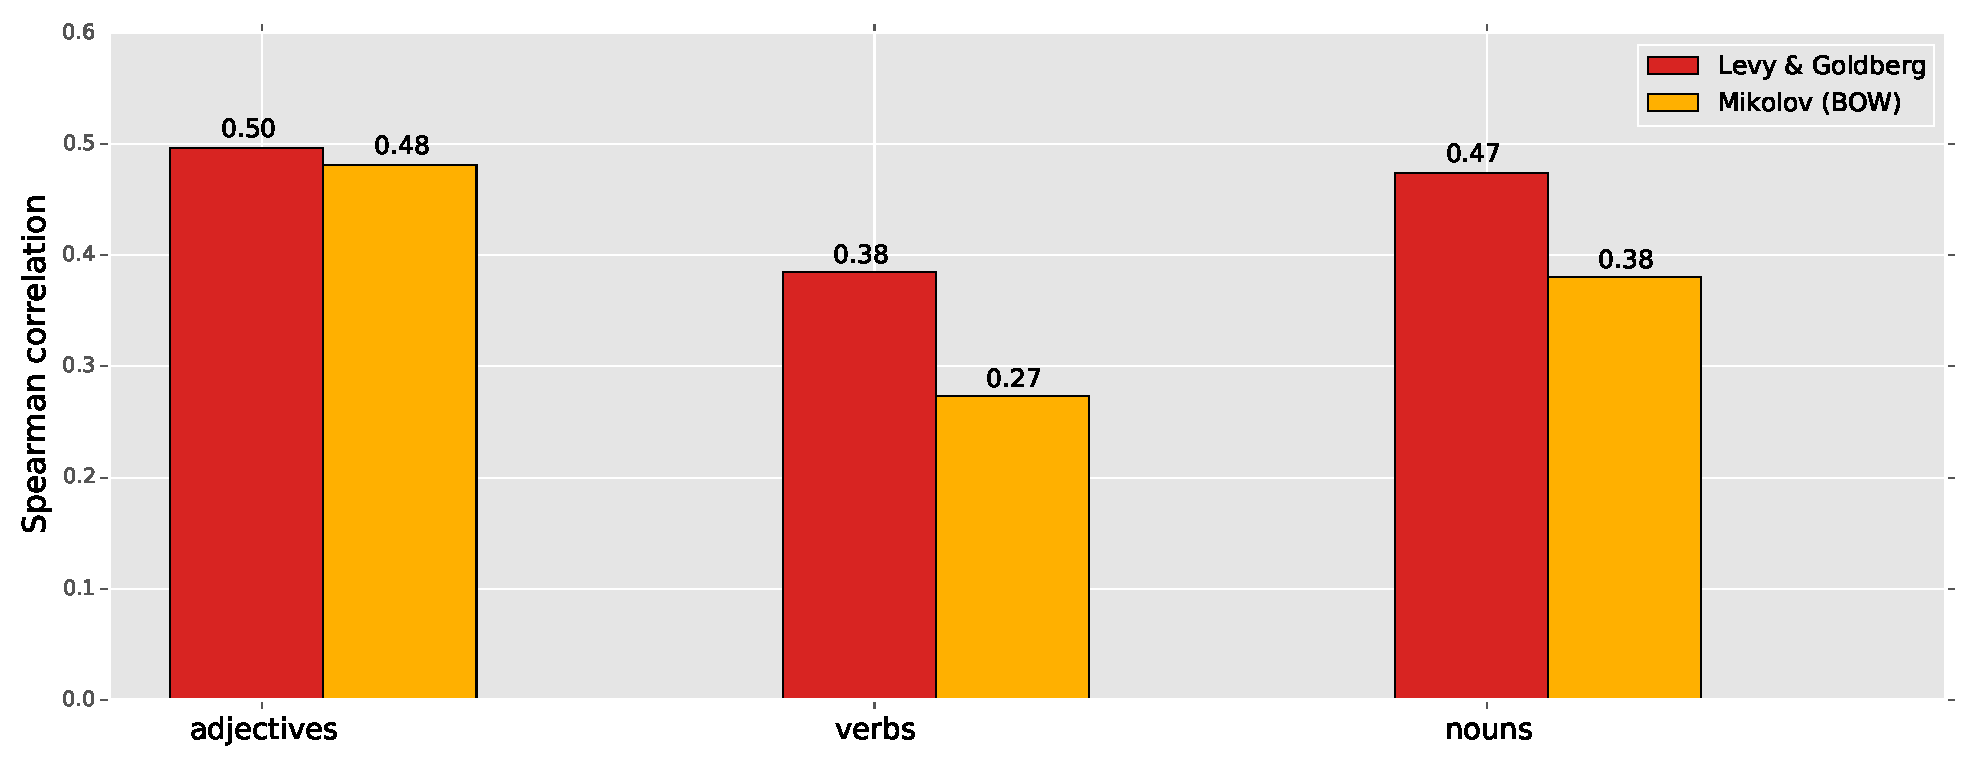
\includegraphics[width = \textwidth,height=5cm]{Chapter_2/New_Figure_2_CL}  \caption{\label{fig12} The importance of dependency-focussed contexts (in the Levy \& Goldberg model) for capturing concepts of different POS, when compared to a standard Skipgram (BOW) model trained on the same Wikipedia corpus.}\end{figure}



\paragraph{\bf Learning concepts of different POS}
\label{begin}

Given the theoretical likelihood of variation in model performance across POS categories noted in Section~\ref{motivation}, I evaluated the \cite{mikolov2013efficient}, VSM and LSA models on the subsets of SimLex-999 containing adjective, noun and verb concept pairs. 

The analyses yield two notable conclusions, as shown in Figure~\ref{fig11}. First, perhaps contrary to intuition, all models estimate the similarity of adjectives better than other concept categories. This aligns with the (also unexpected) observation that humans rate the similarity of adjectives more consistently and with more agreement than other parts of speech (see the dashed lines). However, the parallels between human raters and the models do not extend to verbs and nouns; verb similarity is rated more consistently than noun similarity by humans, but models estimate these ratings more accurately for nouns than for verbs. 

To better understand the linguistic information exploited by models when acquiring concepts of different POS, I also computed performance on the POS subsets of SimLex-999 of the dependency-based model of \cite{levy2014dependency} and the standard skipgram model, in which linguistic contexts are encoded as simple bags-of-words (BOW) \citep{mikolov2013efficient} (trained on the same Wikipedia text). As shown in Figure~\ref{fig12}, dependency-aware contexts yield the largest improvements for capturing verb similarity. This aligns with the cognitive theory of verbs as \emph{relational concepts} \citep{markman1997similar} whose meanings rely on their interaction with (or dependency on) other words or concepts. It is also consistent with research on the automatic acquisition of verb semantics, in which syntactic features have proven particularly important \citep{sun2008verb}.  While a deeper exploration of these effects is beyond the scope of this work, this preliminary analysis again highlights the how the word classes integrated into SimLex-999 are pertinent to a range of questions concerning lexical semantics. 



\paragraph{\bf Learning concrete and abstract concepts}
\label{end}
\begin{figure*}[ht]  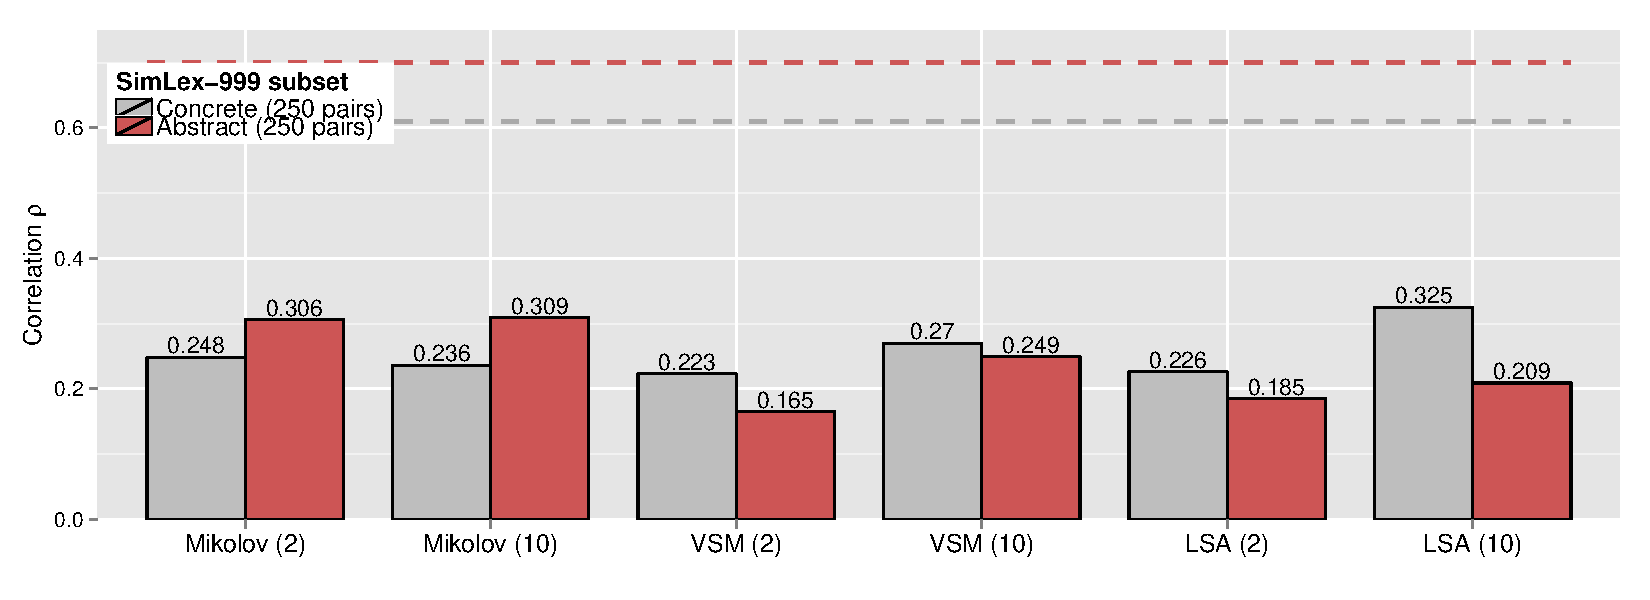
\includegraphics[width = \textwidth,height=5cm]{Chapter_2/Figure_4_CL}  \caption{\label{fig13} Performance of models on concreteness-based subsets of SimLex-999. Window size is indicated in parentheses. Horizontal dashed lines indicate inter-annotator agreement between SimLex-999 annotators on the two subsets.}\end{figure*}


Given the strong interdependence between POS and conceptual concreteness (Figure~\ref{fig1}), I aimed to explore whether the variation in model performance on different POS categories was in fact driven by an underlying effect of concreteness. To do so, I ranked each pair in the SimLex-999 dataset according to the sum of the concreteness of the two words, and compared performance of models on the most concrete and least concrete quartiles according to this ranking (Figure~\ref{fig13}). 

Interestingly, the performance of models on the most abstract and most concrete pairs suggests that the distinction characterised by concreteness is at least partially independent of POS. Specifically, while the Mikolov et al. model was the highest performer on all POS categories, its performance was worse than both the simple VSM and LSA models (of window size 10) on the most concrete concept pairs.

This finding supports the growing evidence for systematic differences in representation and/or similarity operations between abstract and concrete concepts \citep{hill2013concreteness}, and suggests that at least part of these concreteness effects are independent of POS. In particular, it appears that models built from underlying vectors of co-occurrence counts, such as VSMs and LSA, are better equipped to capture the semantics of concrete entities, whereas the embeddings learned by NLMs can better capture abstract semantics. 

\section{Conclusion} 
\label{conclusion}
Although the ultimate test of semantic models should be their utility in downstream applications, the research community can undoubtedly benefit from ways to evaluate the general quality of the representations learned by such models, prior to their integration in any particular system. I have presented SimLex-999, a gold standard resource for the evaluation of semantic representations containing similarity ratings of word pairs of different POS categories and concreteness levels. 

The development of SimLex-999 was principally motivated by two factors. First, as I demonstrated, several existing gold standards measure the ability of models to capture association rather than similarity, and others do not adequately test their ability to discriminate similarity from association. This is despite the many potential applications for accurate similarity-focussed representation learning models. Analysis of the ratings of the 500 SimLex-999 annotators showed that subjects can consistently quantify similarity, as distinct from association, and apply it to various concept types, based on minimal intuitive instructions. 

Second, as I showed, state-of-the-art models trained solely on running-text corpora have now reached or surpassed the human agreement ceiling on WordSim-353 and MEN, the most popular existing gold standards, as well as on RG and WS-Sim. These evaluations may therefore have limited use in guiding or moderating future improvements to distributional semantic models. Nevertheless, there is clearly still room for improvement in terms of the use of distributional models in functional applications. I therefore consider the comparatively low performance of state-of-the-art models on SimLex-999 to be one of its principal strengths. There is clear room under the inter-rating ceiling to guide the development of the next generation of distributional models. 

I conducted a brief exploration of how models might improve on this performance, and verified the hypotheses that models trained on dependency-based input capture similarity more effectively than those trained on running-text input. The evidence that smaller context windows are also beneficial for similarity models was mixed, however. Indeed, I showed that the optimal window size depends on both the general model architecture and the part-of-speech and concreteness of the source concepts. 

The analysis of these hypotheses illustrates how the design of SimLex-999 - covering a principled set of concept categories and including meta-information on concreteness and free-association strength - enables fine-grained analyses of the performance and parameterization of semantic models. However, these experiments only scratch the surface in terms of the possible analyses. Researchers have already adopted the resource as a means of answering a diverse range of questions pertinent to similarity modelling, distributional semantics and representation learning in general (see e.g.~\citep{levy2015improving,wang2015learning}).

\paragraph{What is so special about neural word embeddings?}

Since the analyses in this chapter were conducted, a clearer understanding has emerged of the connection between the word embeddings learned by shallow (log-linear) NLMs and VSMs. The original consensus, based on systematic comparisons~\citep{baroni2014don}, was that shallow neural language models learned `better quality' representations than counting (VSM) approaches. This conclusion is also supported by the analyses presented in this chapter, although Table~\ref{fig8} suggests that the difference (\(\rho = 0.28\) vs. \(\rho = 0.23\)) is not enormous on SimLex-999, and negligible on certain types of concept such as nouns (Table~\ref{fig11}). However, \cite{levy2014neural} have since shown that a non-probabilistic variant of the shallow NLMs (\emph{Skipgram with negative sampling}) effectively minimises the same objective function as a (counting) vector-space model in which sparse count vectors are transformed with SVD. This result formalises some of the intuition expressed in Section~\ref{shallow} concerning how both types of model ultimately exploit the distributional hypothesis. 

The equivalence, or at least close relationship, between shallow NLMs and VSMs made it unclear why studies, including this one, should have observed empirical differences in performance. Thankfully, \cite{levy2015improving} produced a very plausible explanation for this uncertaintly. The aspects of the Skipgram (or CBOW) algorithm that are most critical for the improved performance over VSMs had been excluded from the formal demonstration of equivalence because they seem to be peripheral to the main Skipgram (or CBOW) architecture. For instance, their experiments showed that the position-dependent random sampling of context-words within the fixed window (as described in Section~\ref{shallow}) was an important factor in improved representations in the Skipgram model. Of course, this `stochastic context window' property can also be easily applied to the VSM algorithm. In this way, \cite{levy2015improving} showed that VSMs can be modified to produce representations that are equally rich as those of shallow NLMs. In practice, however, Skipgram and CBOW remain the most popular algorithms for learning word representations from text, perhaps because of the available fast implementations and the much lower memory footprint of the algorithms.    

\paragraph{The future of word representations}

In particular, for models to learn high-quality representations for all linguistic concepts, I believe that future work must uncover ways to explicitly or implicitly infer `deeper', more general conceptual properties such as intentionality, polarity, subjectivity or concreteness \citep{gershmanmetaphor}. However, while improving corpus-based models in this direction is certainly realistic, models that learn exclusively via static text may never reach human-level performance on evaluations such as SimLex-999. Much conceptual knowledge, and particularly that which underlines similarity computations for concrete concepts, appears to be grounded in the perceptual modalities as much as in language \citep{barsalou2003grounding}. At the same time, the deeper conceptual properties such as subjectivity or affect may require a much more active language learning environment, in which learning agents interact (with or without humans), and in which the content of training examples depends on previous output from the model.

Whatever the means by which the improvements are achieved, the ability to acquire concept-level representations that closely align with human cognition is likely to be a crucial part of progress in many directions of NLP and language understanding research, from dialogue and question-answering to machine translation. 

Distributional semantics aims to infer the meaning of words based on the \emph{company they keep} \citep{dist}. However, while words that occur together in text often have associated meanings, these meanings may be very similar or indeed very different. Thus, possibly excepting the population of Argentina, most people would agree that, strictly speaking, \emph{Maradona} is not synonymous with \emph{football} (despite their high rating of 8.62 in WordSim-353). The challenge for the next generation of distributional models may therefore be to infer what is useful from the co-occurrence signal and to overlook what is not. Perhaps only then will models capture most, or even all, of what humans know when they know how to use a language. 
\chapter{Learning word representations from more than text}
% This chapter is about word representations

\section{Introduction}

How can text-based models of word representation be improved in order to achieve human-like performance on evaluations like SimLex-999? Improved algorithms are undoubtedly part of the picture, but it is plausible that models may never acquire human-quality word representations from raw text, however efficient the learning algorithm and however much data they observe. This is because text data as a learning resource lacks various characteristics of the information available to human learners. For instance, much of conceptual acquisition and word learning, particularly at the early stages, apparently involves the unification of linguistic concepts with those acquired via the perceptual system~\citep{barsalou2005situating}. In addition, as the conceptual system develops, humans actively learn via interactions that depend on the current output of the learner, or explicit explanations targetted at the learner, or following a curriculum.Information in this form is not available to the text-based learning algorithms described in the previous chapter. 

In light of these observations, in this chapter I seek to improve the representations acquired by Neural Language Models (NLMs) by training on information sources other than raw text. The analyses focus on word representations because the corresponding models and  and evaluations are better understood, although the conclusions should ultimately extend to phrases and sentences (see Chapter~/ref{CH4}).

 I begin by exploring ways to endow word-learning models with information corresponding to that which is available to the sensory-perceptual system when humans learn concepts. Earlier studies had shown that data from images~\citep{feng2010visual,bruni2012distributional} and data corresponding to other modalities~\cite{kiela2015multi} can enrich distributed representations beyond what can be acquired from text. The analyses presented here extend these studies in two respects. First, it applies a novel algorithm for `mixing' information from different modalities, facilitated by fast NLMs and moderated by word frequency statistics in text. Second, it explicitly considers representations of abstract  (\emph{curiosity}, \emph{loyalty}) as well as concrete (\emph{cat}, \emph{dog}) words. As I show, this is particularly important for language understanding models, since abstract words are much more common than concrete words in adult language. 

In the second part of this chapter, I show how enhanced word representations can be acquired from bilingual text data, using a recently-developed deep sequence-to-sequence learning architecture trained to translate between pairs of European languages. These experiments can be understood as a (crude) cognitive model of bilingual learners, demonstrating how the need to translate between languages might influence or stimulate the acquisition of word concepts. As with the multi-modal learning in the first part of the chapter, I observed show clear quantitative and qualitative differences in word representations acquired via this bilingual learning framework compared with those acquired via equivalent means from (raw) monolingual text. Specifically, the embedding spaces acquired via this bilingual framework are orientated to reflect semantic similarity to a much greater extent than conventional monolingual representation spaces, whose organisation better reflects relatedness. 

\section{Grounded acquisition of abstract concepts from multi-modal data}

Multi-modal models that learn semantic representations from both language and information about the perceptible properties of concepts were originally motivated by parallels with human word learning \citep{andrews2009integrating} and evidence that many concepts are grounded in perception \citep{barsalou2005situating}. The perceptual information in such models is generally mined directly from images \citep{feng2010visual,bruni2012distributional} or from data collected in psychological studies \citep{silberer2012grounded,rollermultimodal}. 

By exploiting the additional information encoded in perceptual input, multi-modal models can outperform language-only models on a range of semantic NLP tasks, including modelling similarity \citep{bruni2014multimodal} and free association \citep{silberer2012grounded}, predicting compositionality \citep{rollermultimodal} and concept categorization \citep{silberer2014learning}. However, to date, this superiority has only been established when evaluating on concrete words such as \emph{house} or \emph{car}, rather than abstract concepts, such as \emph{welcome} or \emph{transport}. Indeed, differences between abstract and concrete processing and representation suggest that conclusions about concrete concept learning may not necessarily hold in the general case~\citep{paivio1991dual,hill2013quantitative}. In this paper, I therefore focus on multi-modal models for learning abstract as well as concrete concept (word) representations.

Although concrete concepts might seem more basic or fundamental, the vast majority of open-class, meaning-bearing words in everyday language are in fact abstract. 72\% of the noun or verb tokens in the British National Corpus \citep{leech1994claws4} are rated by human judges\footnote{Contributors to the USF dataset \citep{nelson2004university}} as more abstract than the noun \emph{war}, for instance, a concept many would already consider to be quite abstract. Moreover, abstract concepts by definition encode higher-level (more general) principles than concrete concepts, which typically reside naturally in a single semantic category or domain \citep{crutch2005abstract}. It is therefore likely that abstract representations may prove highly applicable for multi-task, multi-domain or transfer learning models, which aim to acquire `general-purpose' conceptual knowledge without reference to a specific objective or task \citep{collobert2008unified,mesnil2012unsupervised}. 

Motivated by these observations, I introduce an architecture for learning both abstract and concrete representations that generalizes the Skipgram model of \citep{mikolov2013efficient} from corpus-based  to multi-modal learning. The extended model is designed to reflect aspects of human word learning, in that it introduces more perceptual information about commonly-occurring concrete concepts and less information about rarer concepts. 

I train the model on running-text language and two sources of perceptual descriptors for concrete nouns: the ESPGame dataset of annotated images \citep{von2004labeling} and the CSLB set of concept property norms \citep{devereux2013centre}. I find that the model \emph{combines} information from the different modalities more effectively than previous methods, resulting in an improved ability to model the USF free association gold standard \citep{nelson2004university} for concrete nouns. In addition, the architecture  \emph{propagates} the extra-linguistic input for concrete nouns to improve representations of abstract concepts more effectively than alternative methods. While this propagation can effectively extend the advantage of the multi-modal approach to many more concepts than simple concrete nouns, I observe that the benefit of adding perceptual input appears to decrease as target concepts become more abstract. Indeed, for the most abstract concepts of all, language-only models still provide the most effective learning mechanism.  

Finally, I investigate the optimum quantity and type of perceptual input for such models. Between the most concrete concepts, which can be effectively represented directly in the perceptual modality, and the most abstract concepts, which cannot, I identify a set of concepts that cannot be represented effectively directly in the perceptual modality, but still benefit from perceptual input propagated in the model via concrete concepts. 

My motivation in designing the model and experiments in this section is both practical and theoretical. Taken together, the empirical observations I present are potentially important for optimizing the learning of representations of concrete and abstract concepts in multi-modal models. In addition, they offer a degree of insight into the poorly understood issue of how abstract concepts may be encoded in human memory.    

\subsection{Model Design}

Before describing how the multi-modal architecture encodes and integrates perceptual information, I first describe the underlying corpus-based representation learning model. 

\paragraph{Language-only model} The multi-modal architecture builds on the log-linear Skipgram model proposed by \cite{mikolov2013efficient} and described in Chapter~\ref{CH2}. Here, I extend this architecture via a simple means of introducing perceptual information that aligns with human language learning. Based on the assumption that frequency in domain-general linguistic corpora correlates with the likelihood of `experiencing' a concept in the world \citep{bybee2001frequency,chater2006probabilistic}, perceptual information is introduced to the model whenever designated concrete concepts are encountered in the running-text linguistic input. This has the effect of introducing more perceptual input for commonly experienced concrete concepts and less input for rarer concrete concepts. 

To implement this process,  perceptual information is extracted from external sources and encoded in an associative array \(\bf{P}\), which maps (typically concrete) words \(w\) to bags of perceptual features \({\bf b}(w)\). The construction of this array depends on the perceptual information source; the process for the chosen sources is detailed in Section~\ref{percep_sources}.  

Training the model begins as with the Skipgram model on running-text. When a sentence \(S_m\) containing a word \(w\) in the domain of \(\mathbf{P}\) is encountered, the model completes training on \(S_m\) and begins learning from a perceptual pseudo-sentence \(\hat{S}(w)\).  \(\hat{S_m}(w)\) is constructed  by randomly sampling features from \({\bf b}(w)\) to occupy positions before and instances of \(w\), so that  \(\hat{S_m}(w)\) is the same length as \(S_m\) (see Figure~\ref{examples}). Once training on \(\hat{S_m}(w)\) is completed, the model reverts to the next `real' (linguistic) sentence \(S_{m+1}\), and the process continues. Thus, when a concrete concept is encountered in the corpus, its embedding is first updated based on language (moved incrementally closer to concepts appearing in similar linguistic contexts), and then on perception (moved incrementally closer to concepts with the same or similar perceptual features).  

For greater flexibility, I introduce a parameter \(\alpha\) reflecting the raw quantity of perceptual information relative to linguistic input. When \(\alpha=2\), two pseudo-sentences are generated and inserted for every corpus occurrence of a token from the domain of \(\mathbf{P}\). For non-integral \(\alpha \), the number of sentences inserted is \( \lfloor \alpha \rfloor \), and a further sentence is added with probability \(\alpha - \lfloor \alpha \rfloor \).

In all experiments reported in the following sections I set the window size parameter \(k = 5\) and the minimum frequency parameter \(f = 3\), which guarantees that the model learns embeddings for all concepts in the evaluation sets. While the model learns both target and context-embeddings for each word in the vocabulary, I conduct the experiments with the target embeddings only. I set the dimension parameter \(d = 300 \) as this produces high quality embeddings in the language-only case \citep{mikolov2013efficient}. 

\begin{figure} \(\hat{S}(crocodile) =\)\small{ {\bf Crocodile} legs {\bf crocodile} teeth {\bf crocodile} teeth {\bf crocodile} scales {\bf crocodile} green {\bf crocodile}. \\ \\ \(\hat{S}(screwdriver)=\) { \bf Screwdriver} handle {\bf screwdriver} flat  {\bf screwdriver} long {\bf screwdriver}  handle {\bf screwdriver}  head. } \caption{\label{examples} Example pseudo-sentences generated for training the model.}\end{figure}

\subsection{Information sources}
\label{percep_sources}

We construct the associative array of perceptual information \(\mathbf{P}\) from two sources typical of those used for multi-modal semantic models.

\paragraph{ESPGame dataset} The ESP-Game dataset (ESP) \citep{von2004labeling} consists of 100,000 images, each annotated with a list of lexical concepts that appear in that image. For any concept \(w\) identified in an ESP image, I construct a corresponding bag of features \({\bf b}(w)\). For each ESP image \(I\) that contains \(w\), I append the other concept tokens identified in \(I\) to \({\bf b}(w)\). Thus, the more frequently a concept co-occurs with \(w\) in images, the more its corresponding lexical token occurs in \({\bf b}(w)\). The array \(\mathbf{P_{ESP}}\) in this case then consists of the  \( (w,  {\bf b}(w) ) \) pairs.

\paragraph{CSLB Property Norms} The Centre for Speech, Language and the Brain norms (CSLB) \citep{devereux2013centre} is a recently-released dataset containing semantic properties for 638 concrete concepts produced by human annotators. The CSLB dataset was compiled in the same way as the \cite{mcrae2005semantic} property norms used widely in multi-modal models \citep{silberer2012grounded,rollermultimodal}; I use CSLB because it contains more concepts. For each concept, the proportion of the 30 annotators that produced a given feature can also be employed as a measure of the strength of that feature.

When encoding the CSLB data in \(\mathbf{P}\), I first map properties to lexical forms (e.g. \emph{is\_green} becomes \emph{green}). By directly identifying perceptual features and linguistic forms in this way, I treat features observed in the perceptual data as (sub)concepts to be acquired via the same multi-modal input streams and stored in the same domain-general memory as the evaluation concepts. This non-modular characterisation of semantic memory  in fact corresponds to a view of cognition that is sometimes disputed \citep{fodor1983modularity}. In future studies I hope to compare the present approach to architectures with domain-specific conceptual memories. 

For each concept \(w\) in CSLB, I then construct a feature bag \({\bf b}(w)\) by appending lexical forms to \({\bf b}(w)\) such that the count of each feature word is equal to the strength of that feature for \(w\). Thus, when features are sampled from \({\bf b}(w)\) to create pseudo-sentences (as detailed previously) the probability of a feature word occuring in a sentence reflects feature strength. The array \(\mathbf{P_{CSLB}}\) then consists of all \( (w,  {\bf b}(w) ) \) pairs.

\paragraph{Linguistic input} The linguistic input to all models is the 400m word Text8 Corpus\footnote{From http://mattmahoney.net/dc/textdata.html} of Wikipedia text, split into sentences and with punctuation removed. 



 \begin{table}[t]\begin{center}\begin{tabular}{c|ccc|c}


\multicolumn{2}{c}{\bf ESPGame} &\multicolumn{1}{c}{} & \multicolumn{2}{c}{\bf CSLB}\\
 \underline{Image 1} &  \underline{Image 2} & &  \underline{Crocodile} & \underline{Screwdriver} \\ 
\footnotesize{red} &  \footnotesize{wreck} &  &  \footnotesize{has 4 legs (7)} &  \footnotesize{has handle (28)} \\ 
\footnotesize{chihuaua} &  \footnotesize{cyan} & &  \footnotesize{has tail (18)} &  \footnotesize{has head (5)} \\ 
\footnotesize{eyes} &  \footnotesize{man} & &  \footnotesize{has jaw (7)} & \footnotesize{is long (9)} \\ 
\footnotesize{little} &  \footnotesize{crash} & &  \footnotesize{has scales (8)} &   \footnotesize{is plastic (18)} \\ 
\footnotesize{ear} &  \footnotesize{accident} & &  \footnotesize{has teeth (20)} & \footnotesize{is metal (28)} \\ 
\footnotesize{nose}  &  \footnotesize{street} & &  \footnotesize{is green (10}) &  \\ 
\footnotesize{small} &   & & \footnotesize{is large (10)} &    \\ 






\end{tabular}\end{center}\caption{\label{font-table} Concepts identified in images in the ESP Game (left) and features produced for concepts by human annotators in the CSLB dataset (with feature strength, max=30).}\end{table}







\subsection{Evaluation}

SimLex-999 was produced after these experiments were carried out. I therefore evaluated the quality of representations by how well they reflect the University of South Florida Norms (USF) \citep{nelson2004university} free association scores. These norms measure the strenght of association between over 40,000 concept pairs, many of which, importantly, contain abstract concepts. Prior to SimLex-999, they had been widely used in NLP to evaluate semantic representations \citep{andrews2009integrating,feng2010visual,silberer2012grounded,rollermultimodal}. Each concept that I extracted from the USF database was also rated for conceptual concreteness on a Likert scale of 1-7 by at least 10 human annotators. Following previous studies \citep{huang2012improving,silberer2012grounded}, I measured the (Spearman \(\rho\)) correlation between association scores and the cosine similarity of vector representations.

 \begin{table}[t]\begin{center}\begin{tabular}{l|l|c}



\bf Concept 1 & \bf Concept 2 & \bf Assoc. \\
 \hline 
abdomen \footnotesize{ (6.83)} & stomach \footnotesize{ (6.04)} & 0.566 \\
throw \footnotesize{  (4.05)} & ball  \footnotesize{ (6.08)} & 0.234 \\
hope \footnotesize{  (1.18)} & glory \footnotesize{ (3.53)} & 0.192 \\
egg \footnotesize{ (5.79)} & milk \footnotesize{ (6.66)} & 0.012 \\



\end{tabular}\end{center}\caption{\label{font-table} Example concept pairs (with mean concreteness rating) and free-association scores from the USF dataset.}\end{table}






I created separate abstract and concrete concept lists by ranking the USF concepts according to concreteness and sampling at random from the first and fourth quartiles. I also introduced a complementary noun/verb dichotomy,\footnote{Based on the majority POS-tag of words in the lemmatized British National Corpus \citep{leech1994claws4}} on the intuition that information propagation may occur differently from noun to noun or from noun to verb (because of their distinct structural relationships in sentences). The abstract/concrete and noun/verb dichotomies yielded four distinct concept lists. For consistency, the concrete noun list was filtered so that all concrete noun concepts \(w\) have perceptual representations {\bf b}(w) in both  \(\mathbf{P_{ESP}}\) and  \(\mathbf{P_{CSLB}}\). For each of the four resulting concept lists \(C\) (concrete/abstract, noun/verb), a corresponding set of evaluation pairs  \( \{ (w_1, w_2) \in USF :  w_1, w_2 \in C\}\) was extracted (see Table~\ref{set_details} for details). 



 \begin{table}[t]\begin{center}\begin{tabular}{l|r|r|p{2.1cm}}



\bf Concept Type & \bf  List & \bf Pairs & \bf Examples \\ 

\hline concrete nouns & 541 & 1418 & \emph{yacht, cup} \\

abstract nouns & 100 & 295 & \emph{fear, respect} \\

all nouns & 666 & 1815 & \emph{fear, cup} \\

concrete verbs & 50 & 66 & \emph{kiss, launch} \\

abstract verbs & 50 & 127 & \emph{differ, obey} \\

all verbs & 100 & 221 & \emph{kiss, obey} \\

\end{tabular}\end{center}\caption{\label{set_details} Details the subsets of USF data used in the evaluations}\end{table}






\subsection{Results and Discussion}

Our experiments were designed to answer four questions, outlined in the following subsections: (1) Which model architectures perform best at \emph{combining} information pertinent to multiple modalities when such information exists explicitly (as common for concrete concepts)? (2) Which model architectures best propagate perceptual information to concepts for which it does not exist explicitly (as is common for abstract concepts)? (3) Is it preferable to include all of the perceptual input that can be obtained from a given source, or to filter this input stream in some way? (4) How much perceptual vs. linguistic input is optimal for learning various concept types? 

\subsection{Combining information sources} 
\label{conc1}
To evaluate the approach as a method of information combination I compared its performance on the concrete noun evaluation set against alternative methods. When implementing the alternatives, I first encoded the perceptual input directly into sparse feature vectors, with coordinates for each of the 2,726 features in CSLB and for each of the 100,000 images in ESP. 

The first alternative was simple concatenation of these perceptual vectors with linguistic vectors embeddings learned by the \cite{mikolov2013efficient} model on the Text8 Corpus. In the second alternative, proposed for multi-modal models by \cite{silberer2012grounded}, Canonical Correlation Analysis (CCA) \citep{hardoon2004canonical} was applied to the vectors of both modalities. This yielded reduced-dimensionality representations that preserve underlying inter-modal correlations, which are then concatenated. The final alternative, proposed by \cite{bruni2014multimodal} involved applying Singular Value Decomposition (SVD) to the matrix of concatenated multi-modal representations, yielding smoothed representations.\footnote{CCA was implemented using the \emph{CCA} package in R. SVD was implemented using the Python \emph{sparsesvd} package, with truncation factor \(k=1024\) as per \cite{bruni2014multimodal}.}

I compared these alternatives to the proposed model with \(\alpha = 1\). In The CSLB and ESP models, all training pseudo-sentences were generated from the arrays \(\mathbf{P_{CSLB}}\) and \(\mathbf{P_{ESP}}\) respectively. In the models classed as \emph{CSLB\&ESP}, a random choice between \(\mathbf{P_{CSLB}}\) and \(\mathbf{P_{ESP}}\) was made every time perceptual input was included (so that the overall quantity of perceptual information was the same). 

As shown in Figure~\ref{main_results} (left side), the embeddings learned by the model achieved a higher correlation with the USF data than simple concatenation, CCA and SVD regardless of perceptual input source. With the optimal perceptual source (ESP only), for instance, the correlation was 11\% higher that the next best alternative method, CCA. 

One possible factor behind this improvement is that, in the model, the learned representations fully integrate the two modalities, whereas for both CCA and the concatenation method each representation feature (whether of reduced dimension or not) corresponds to a particular modality. This deeper integration may help the architecture to overcome the challenges inherent in information combination such as inter-modality differences in information content and representation sparsity.   


\subsection{Propagating input to abstract concepts} 
\label{conc2}
To test the process of information propagation in the model, I evaluated the learned embeddings of more abstract concepts. I compared the approach with two recently-proposed alternative methods for inferring perceptual features when explicit perceptual information is unavailable. 

\paragraph{Johns and Jones} In the method of \cite{johns2012perceptual}, pseudo-perceptual representations for target concepts without a perceptual representations (uni-modal concepts) are inferred as a weighted average of the perceptual representations of concepts that do have such a representation (bi-modal concepts). 

In the first step of their two-step method, for each uni-modal concept  \(\bf k\), a quasi-perceptual representation is computed as an average of the perceptual representations of bi-modal concepts, weighted by the proximity between each of these concepts and \( \bf k\)\[{\bf k}^p = \sum_{{\bf c} \in \bar{C}} S({\bf k}^l,{\bf c}^l)^\lambda \cdot {\bf c}^p  \] where \(  \bar{C} \) is the set of bi-modal concepts, \({\bf c}^p\) and  \({\bf k}^p\) are the perceptual representations for \(\bf c\) and \(\bf k\) respectively, and  \({\bf c}^l\) and \({\bf k}^l\) the linguistic representations. The exponent parameter \(\lambda \) reflects the learning rate. 

In step two, the initial quasi-perceptual representations are inferred for a second time, but with the weighted average calculated over the perceptual or initial quasi-perceptual representations of all other words, not just those that were orignally bi-modal. As with \cite{johns2012perceptual}, I set the learning rate parameter \( \lambda\) to be 3 in the first step and 13 in the second.  


\paragraph{Ridge Regression} A simpler method for mixing modalities can be achieved using ridge regression. Ridge regression is a variant of least squares regression in which a regularization term is added to the training objective to favor solutions with certain properties. 

For bimodal concepts of dimension \(n_p\), I used ridge regression to learn \(n_p\) linear functions \( f_i: \mathbb{R}^{n_l} \to \mathbb{R} \) that map the linguistic representations (of dimension \(n_l\)) to a particular perceptual feature \(i\). These functions were then applied together to map the linguistic representations of uni-modal concepts to full quasi-perceptual representations.

Following~\cite{hill2014multi}, I took the Euclidian \( l_2 \) norm of the inferred parameter vector as the regularization term. This ensured that the regression favors lower coefficients and a smoother solution function, which should provide better generalization performance than simple linear regression. The objective for learning the \( f_i \) was then to minimize \[ \| {\bf a}X - Y_i \|_2^2 + \|{\bf a}\|_2^2 \] where \( {\bf a}\) is the vector of regression coefficients, \( X \) is a matrix of linguistic representations and \(  Y_i \) a vector of the perceptual feature \(i\) for the set of bi-modal concepts.

\paragraph{Comparisons} I applied the Johns and Jones method and ridge regression starting from linguistic embeddings acquired by the \cite{mikolov2013efficient} model on the Text8 Corpus, and concatenated the resulting pseudo-perceptual and linguistic representations. The perceptual input for all models was limited to concrete nouns (i.e. concrete nouns were the only bi-modal concepts in the models).

 \begin{figure*}  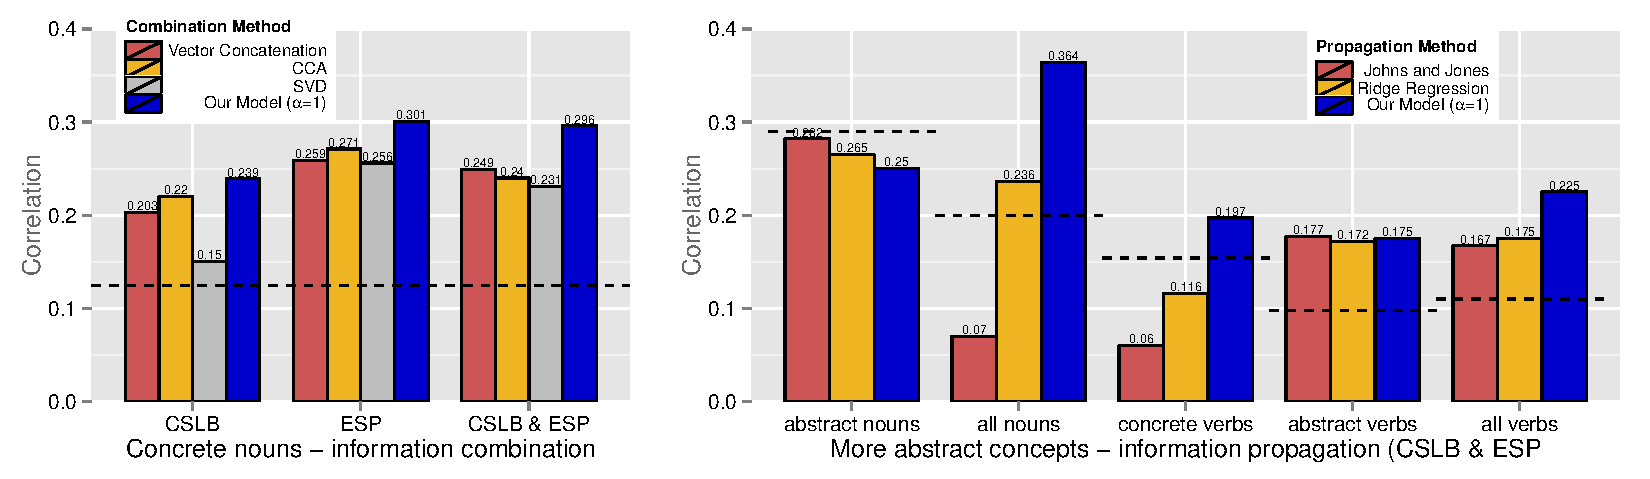
\includegraphics[width = \textwidth]{Chapter_3/Graph_1_EMNLP2014}  \caption{\label{main_results} The proposed approach compared with other methods of information combination (left) and propagation. Dashed lines indicate language-only model baseline.}\end{figure*}

Figure~\ref{main_results} (right side) illustrates the propagation performance of the three models. While the correlations overall may seem somewhat low, this is a consequence of the difficulty of modeling the USF data. In fact, the performance of both the language-only model and the multi-modal extension across the concept types, ranging from \(0.18 - 0.36\), is equal to or higher than equivalent models evaluated on the same data previously \citep{feng2010visual,silberer2012grounded,silberer2013models}. 

For learning representations of concrete verbs, the approach achieves a 69\% increase in performance over the next best alternative. The performance of the model on abstract verbs is marginally inferior to Johns and Jones' method. Nevertheless, the clear advantage for concrete verbs makes the model the best choice for learning representations of verbs in general, as shown by performance on the set \emph{all verbs}, which also includes mixed abstract-concrete pairs. 

The model is also marginally inferior to alternative approaches in learning representations of abstract nouns. However, in this case, no method improves on the linguistic-only baseline. It is possible that perceptual information is simply so removed from the core semantics of these concepts that they are best acquired via the linguistic medium alone, regardless of learning mechanism. The moderately inferior performance of the method in such cases is likely caused by its greater inherent inter-modal dependence compared with methods that simply concatenate uni-modal representations. When the perceptual signal is of low quality, this greater inter-modal dependence allows the linguistic signal to be obscured. The trade-off, however, is the higher quality joint representations when the perceptual signal is of higher-quality, exemplified by the fact that the proposed approach outperforms alternatives on the set \emph{all nouns}, which includes the more concrete nouns. 

\subsection{Direct representation vs. propagation}
\label{conc3}

 \begin{figure*}[t] 

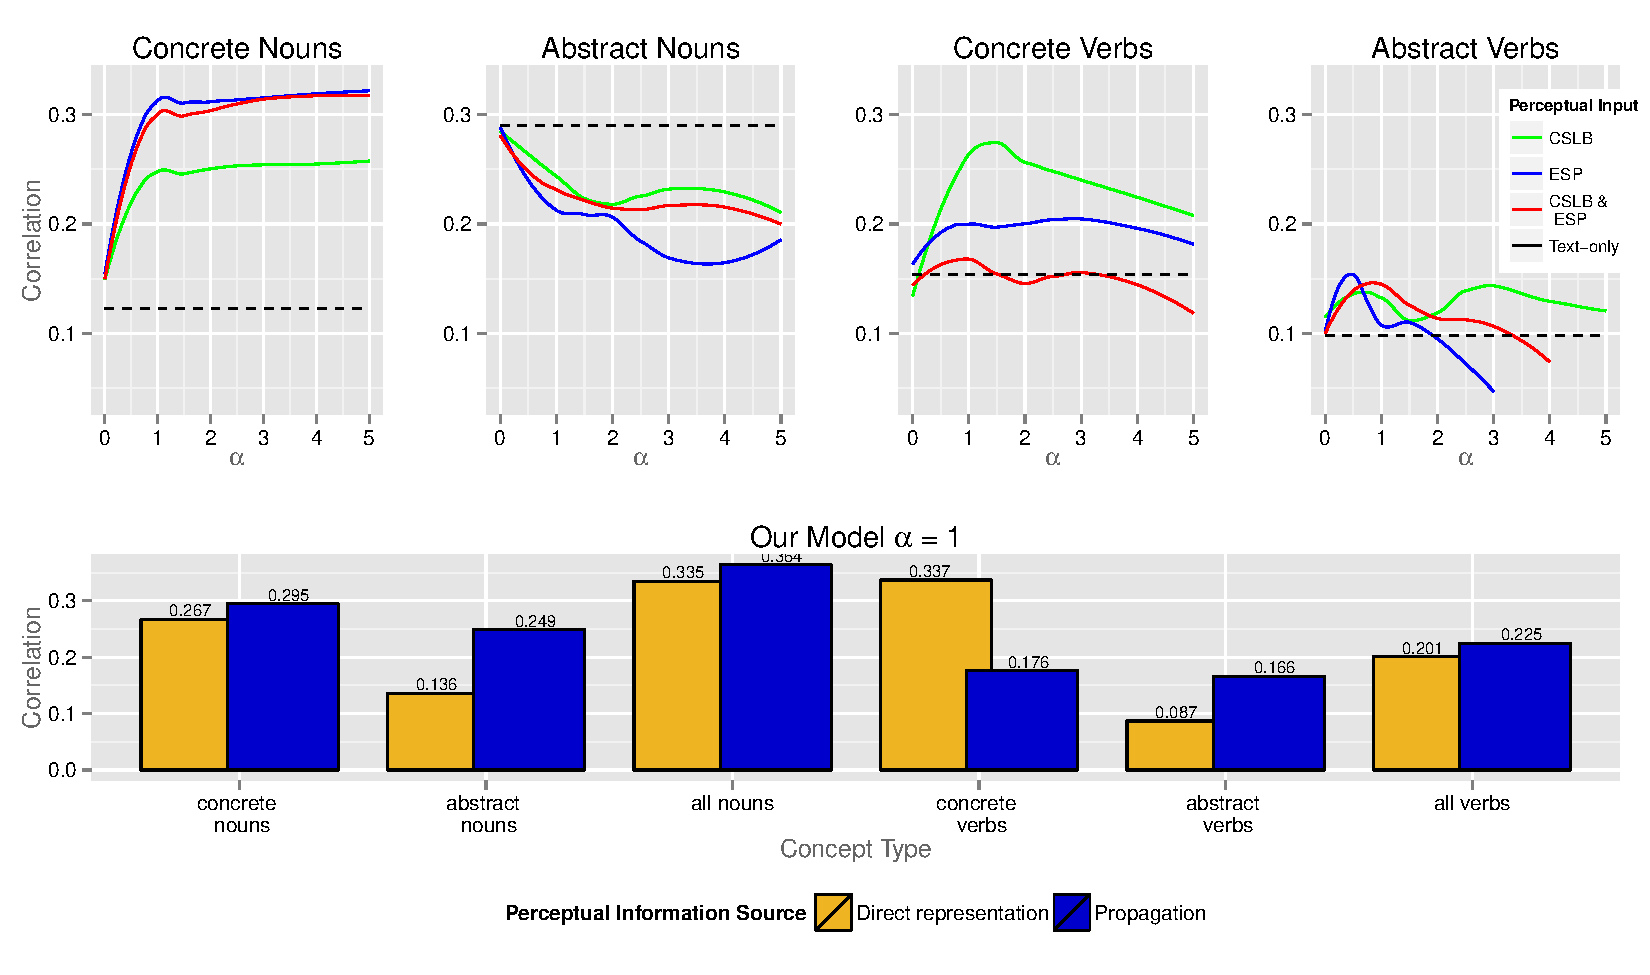
\includegraphics[width = \textwidth]{Chapter_3/Graph_2_EMNLP2014}  

\caption{\label{repprop} {\bf Top}: Comparing the strategy of directly representing abstract concepts from perceptual information where available (yellow bars) vs. propagating via concrete concepts. {\bf Bottom}: The effect of increasing \(\alpha\) on correlation with USF pairs (Spearman \(\rho\)) for each concept type. Horizontal dashed lines indicate language-only model baseline.}

\end{figure*}

Although property norm datasets such as the CSLB data typically consist of perceptual feature information for concrete nouns only, image-based datasets such as ESP do contain information on more abstract concepts, which was omitted from the previous experiments. Indeed, image banks such as Google Images contain millions of photographs portraying quite abstract concepts, such as \emph{love} or \emph{war}. On the other hand, encodings or descriptions of abstract concepts are generally more subjective and less reliable than those of concrete concepts \citep{katja2005content}. I therefore investigated whether or not it is preferable to include this additional information as model input or to restrict perceptual input to concrete nouns as previously.    

Of the evaluation sets, it was possible to construct from ESP (and add to \(\mathbf{P_{ESP}}\)) representations for all of the concrete verbs, and for approximately half of the abstract verbs and abstract nouns. Figure~\ref{repprop} (top), shows the performance of a the model trained on all available perceptual input versus the model in which the perceptual input was restricted to concrete nouns. 

The results reflect a clear manifestation of the abstract/concrete distinction. Concrete verbs behave similarly to concrete nouns, in that they can be effectively represented directly from perceptual information sources. The information encoded in these representations is beneficial to the model and increases performance. In contrast, constructing `perceptual' representations of abstract verbs and abstract nouns directly from perceptual information sources is clearly counter-productive (to the extent that performance also degrades on the combined sets \emph{all nouns} and \emph{all verbs}). It appears in these cases that the perceptual input acts to obscure or contradict the otherwise useful signal inferred from the corpus.

As shown in the previous section, the inclusion of any form of perceptual input inhibits the learning of abstract nouns. However, this is not the case for abstract verbs. Our model learns higher quality representations of abstract verbs when perceptual input is restricted to concrete nouns than when no perceptual input is included whatsoever \emph{and} when perceptual input is included for both concrete nouns and abstract verbs. This supports the idea of a gradual scale of concreteness: the most concrete concepts can be effectively represented directly in the perceptual modality; somewhat more abstract concepts cannot be represented directly in the perceptual modality, but have representations that are improved by propagating perceptual input from concrete concepts via language; and the most abstract concepts are best acquired via language alone.   

\subsection{Source and quantity of perceptual input} For different concept types, I tested the effect of varying the proportion of perceptual to linguistic input (the parameter \(\alpha\)). Perceptual input was restricted to concrete nouns as in Sections~\ref{conc1}-\ref{conc3}.

As shown in Figure~\ref{repprop}, performance on concrete nouns improves (albeit to a decreasing degree) as \( \alpha \) increases. When learning concrete noun representations, linguistic input is apparently redundant if perceptual input is of sufficient quality and quantity. For the other concept types, in each case there is an optimal value for \( \alpha \) in the range \(0.5 - 0.2\), above which perceptual input obscures the linguistic signal and performance degrades. The proximity of these optima to 1 suggests that  for optimal learning, when a concrete concept is experienced approximately equal weight should be given to available perceptual and linguistic information. 

\subsection{Conclusions}

Motivated by the notable prevalence of abstract concepts in everyday language, and their likely importance to flexible, general-purpose representation learning, this section has investigated how abstract and concrete representations can be acquired by multi-modal models. In doing so, I presented a simple and easy-to-implement architecture for acquiring semantic representations of both types of concept from linguistic and perceptual input. 

While NLMs have been applied to the problem of multi-modal representation learning previously \citep{srivastava2012multimodal,wu2013online} the model and experiments develop this work in several important ways. First, I addressed the problem of learning abstract concepts. By isolating concepts of different concreteness and part-of-speech in the evaluation sets, and separating the processes of information combination and propagation, I demonstrate that the multi-modal approach is indeed effective for some, but perhaps not all, abstract concepts. In addition, the model introduces a clear parallel with human language learning. Perceptual input is introduced precisely when concrete concepts are `experienced' by the model in the corpus text, much like a language learner experiencing concrete entities via sensory perception.  

Taken together, the findings indicate the utility of distinguishing three concept types when learning representations in the multi-modal setting. 

\paragraph{Type I} Concepts that can be effectively represented directly in the perceptual modality. For such concepts, generally concrete nouns or concrete verbs, the proposed approach provides a simple means of combining perceptual and linguistic input. The resulting multi-modal representations are of higher quality than those learned via other approaches, resulting in a performance improvement of over 10\% in modelling free association.

\paragraph{Type II} Concepts, including abstract verbs, that cannot be effectively represented directly in the perceptual modality, but whose representations can be improved by joint learning from linguistic input and perceptual information about related concepts. Our model can effectively propagate perceptual input (exploiting the relations inferred from the linguistic input) from Type I concepts to enhance the representations of Type II concepts above the language-only baseline. Because of the frequency of abstract concepts, such propagation extends the benefit of the multi-modal approach to a far wider range of language than models based solely in the concrete domain. 

\paragraph{Type III} Concepts, such as abstract nouns, which are more effectively learned via language-only models than multi-modal models. Neither the model I introduce here nor other proposed propagation methods achieve an improvement in representation quality for these concepts over the language-only baseline. Of course, it is an empirical question whether a multi-modal approach could ever enhance the representation learning of these concepts, one with potential implications for cognitive theories of grounding (a topic of much debate in psychology \citep{grafton2009embodied,barsalou2010grounded}). 

Additionally, I investigated the optimum type and quantity of perceptual input for learning concepts of different types. I showed that too much perceptual input can result in degraded representations. For concepts of type I and II, the optimal quantity resulted from setting \(\alpha = 1\); i.e. whenever a concrete concept was encountered, the model learned from an equal number of language-based and perception-based examples. While I make no formal claims here, such observations may ultimately provide insight into human language learning and semantic memory. 

% \section{Multi-modal fusion based on image dispersion}

% include your own bib file like this:


\section{Learning word representations from bilingual data using encoder-decoder models}

Recent empirical~\citep{baroni2014don,levy2015improving} and theoretical~\citep{levy2014neural} studies have yielded a better understanding of how log-linear NLMs such as Skipgram and CBOW acquire meaningful conceptual semantics. However, much less is known about the word embeddings learned by deeper NLMs with more nuanced or complex objectives. In this section, I take some steps in this direction by considering the embeddings learned by architectures with a very different objective function to the Skipgram or CBOW models: \emph{neural machine translation} (NMT) \emph{models}. NMT models have recently emerged as an alternative to statistical, phrase-based translation models, and are beginning to achieve impressive translation performance~\citep{kalchbrenner13emnlp,devlin2014fast,Sutskever2014sequence}.

We show that NMT models are not only a potential new direction for machine translation, but are also an effective means of learning word embeddings. Specifically, NMT word embeddings encode information relating to conceptual similarity (rather than non-specific relatedness or association) and lexical syntactic role more effectively than embeddings from monolingual NLMs. I demonstrate that these properties persist when translating between different language pairs (English-French and English-German). Further, based on the observation of subtle language-specific effects in the embedding spaces, I conjecture as to why similarity dominates over other semantic relations in translation embedding spaces. Finally, I discuss a potential limitation of the application of NMT models for embedding learning - the computational cost of training large vocabularies of embeddings - and show that a novel method for overcoming this issue preserves the aforementioned properties of translation-based embeddings. 

% I show that the precise information encoFinally, I consider ways to combine the distinct information encoded in language-model embeddings and those from translation embeddings. And I consider ways to overcome two important limitations of neural translation models as embedding-learning architectures: the computational difficulty in learning large vocabularies of embeddings, and the requirement for sentence-aligned bilingual training corpora.   

\subsection{Neural Machine Translation Models}

The objective of NMT models is to generate an appropriate sentence in a target language \(S_t\)  given a sentence \(S_s\) in the source language (see e.g.~\citep{kalchbrenner13emnlp,Sutskever2014sequence}). As a by-product of learning to meet this objective, NMT models learn distinct sets of embeddings for the vocabularies \(V_ s\) and \(V_t\) in the source and target languages respectively.

Observing a training case \((S_s, S_t)\), these models represent \(S_s\) as an ordered sequence of embeddings of words from \(V_s\). The sequence for \(S_s\) is then encoded into a single representation \(R_S\).\footnote{Alternatively, subsequences (phrases) of \(S_s\) may be encoded at this stage in place of the whole sentence~\citep{bahdanau2014neural}.} Finally, by referencing the embeddings in \(V_t\), \(R_S\) and a representation of what has been generated thus far, the model decodes a sentence in the target language word by word. If at any stage the decoded word does not match the corresponding word in the training target \(S_t\), the error is recorded. The weights and embeddings in the model, which together parameterise the encoding and decoding process, are updated based on the accumulated error once the sentence decoding is complete. 

Although NMT models can differ in their low-level architecture~\citep{kalchbrenner13emnlp,Cho2014,bahdanau2014neural}, the translation objective exerts similar pressure on the word embeddings in all cases. The source language embeddings must be such that the model can combine them to form single representations for ordered sequences of multiple words (which in turn must enable the decoding process). The target language embeddings must facilitate the process of decoding these representations into correct target-language sentences.    

\subsection{Other bilingual models of learning word representations}
Before the advent of effective end-to-end NMT systems, several models had been developed with the specific goal of acquiring distributed word representations from bilingual corpora, aligned at the document, paragraph or word level~\citep{Haghighi2008Learning,vulic2011identifying,mikolov2013exploiting,Hermann:2014:ICLR,lauly2014autoencoder}. While these approaches rely on the same training data as NMT models, one important difference is that they represent the words from two different languages in single common vector space so that words in one language are close to words with similar or related meanings in the other (this is not the case for NMT models, where the source and target language word embeddings inhabit distinct vector spaces). The resulting multilingual embedding spaces have been effectively applied to bilingual lexicon extraction~\citep{Haghighi2008Learning,vulic2011identifying,mikolov2013exploiting} and document classification~\citep{Klementiev,Hermann:2014:ICLR,lauly2014autoencoder,Kocisky:2014}.

For comparison, we focus on two representatives of this class of (non-NMT) bilingual model. The first is that of \cite{Hermann:2014:ICLR}, whose embeddings improve on the performance of~\cite{Klementiev} in document classification applications. As with NMT models, this model can be trained directly on bitexts aligned only at the sentence rather than word level. When training, for aligned sentences \(S_E\) and \(S_F\) in different languages, the model computes representations \(R_E\) and \(R_F\) by summing the embeddings of the words in \(S_E\) and \(S_F\) respectively. The embeddings are then updated to minimise the divergence between \(R_E\) and \(R_F\) (since they convey a common meaning). A noise-contrastive loss function ensures that the model does not arrive at trivial (e.g. all zero) solutions to this objective.~\cite{Hermann:2014:ICLR} show that, despite the lack of prespecified word alignments, words in the two languages with similar meanings converge in the bilingual embedding space.\footnote{The models of \cite{lauly2014autoencoder} and \cite{Hermann:2014:ICLR} both aim to minimise the divergence between source and target language sentences represented as sums of word embeddings. Because of these similarities, I do not compare with both in this paper.}

The second model I examine is that of \cite{faruqui2014improving}. Unlike the models described above, \cite{faruqui2014improving} showed explicitly that projecting word embeddings from two languages (learned independently) into a common vector space can favourably influence the orientation of word embeddings when considered in their monolingual subspace; i.e relative to other words in their own language. In contrast to the other models considered in this paper, the approach of~\cite{faruqui2014improving} requires bilingual data to be aligned at the word level.

\subsection{Experiments}

To learn translation-based embeddings, I trained two different NMT models. The first is the RNN encoder-decoder, \emph{RNNenc}~\citep{Cho2014}, which uses a recurrent neural network (RNN) to encode all of the source sentence into a single vector on which the decoding process is conditioned. The second is the \emph{RNN Search} architecture~\citep{bahdanau2014neural}, which was designed to overcome limitations exhibited by the RNN encoder-decoder when translating very long sentences. RNN Search includes an \emph{attention} mechanism, an additional feed-forward network that learns to attend to different parts of the source sentence when decoding each word in the target sentence.\footnote{Access to source code and limited GPU time prevented me from training and evaluating the embeddings from other NMT models such as that of~\cite{kalchbrenner13emnlp},~\cite{devlin2014fast} and \cite{Sutskever2014sequence}. The underlying principles of encoding-decoding also apply to these models, and I expect the embeddings would exhibit similar properties to those analysed here.} Both models were trained on a 348m word corpus of English-French sentence pairs or a 91m word corpus of English-German sentence pairs.\footnote{These corpora were produced from the WMT ’14 parallel data after conducting the data-selection procedure described by~\cite{Cho2014}. } 

To explore the properties of bilingual embeddings learned via objectives other than direct translation, I trained the \emph{BiCVM} model of~\cite{Hermann:2014:ICLR} on the same data, and also downloaded the projected embeddings of~\cite{faruqui2014improving}, \emph{FD}, trained on a bilingual corpus of comparable size (\(\approx 300\) million words per language).\footnote{Available from \url{http://www.cs.cmu.edu/~mfaruqui/soft.html}. The available embeddings were trained on English-German aligned data, but the authors report similar to for English-French.} Finally, to compare with monolingual word embedding models, I trained a conventional skipgram model~\citep{mikolov2013distributed} and its \emph{Glove} variant~\citep{Pennington2014} for the same number of epochs on the English half of the bilingual corpus. 

To analyse the effect on embedding quality of increasing the quantity of training data, I then trained the monolingual models on increasingly large random subsamples of Wikipedia text (up to a total of 1.1bn words). Lastly, I extracted embeddings from a full-sentence language model, \emph{CW},~\citep{collobert2008unified}, which was trained for several months on the same Wikipedia 1bn word corpus. Note that increasing the volume of training data for the bilingual (and NMT) models was not possible because of the limited size of available sentence-aligned bitexts. 
 
\subsubsection{Similarity and relatedness modelling}

As in previous studies~\citep{Agirre2009,bruni2014multimodal,baroni2014don}, the initial evaluations involved calculating pairwise (cosine) distances between embeddings and correlating these distances with (gold-standard) human judgements of the strength of relationships between concepts. For this I used three different gold standards: WordSim-353~\citep{Agirre2009}, MEN~\citep{bruni2014multimodal} and SimLex-999~\citep{hill2014simlex}. Recall that there is a clear distinction between WordSim-353 and MEN, on the one hand, and SimLex-999, on the other, in terms of the semantic relationship that they quantify. For both WordSim-353 and MEN, annotators were asked to rate how \emph{related} or \emph{associated} two concepts are. Consequently, pairs such as [\emph{clothes}-\emph{closet}], which are clearly related but ontologically dissimilar, have high ratings in WordSim-353 and MEN. In contrast, such pairs receive a low rating in SimLex-999, where only genuinely \emph{similar} concepts, such as [\emph{coast}- \emph{shore}], receive high ratings. 

Table~\ref{table:perf} shows the correlations of NMT (English-French) embeddings, other bilingually trained embeddings and monolingual embeddings with these three lexical gold-standards. NMT outperform monolingual embeddings, and, to a lesser extent, the other bilingually trained embeddings, on SimLex-999. However, this clear advantage is not observed on MEN and WordSim-353, where the projected embeddings of~\cite{faruqui2014improving}, which were tuned for high performance on WordSim-353, perform best. Given the aforementioned differences between the evaluations, this suggests that bilingually-trained embeddings, and NMT based embeddings in particular, better capture similarity, whereas monolingual embedding spaces are orientated more towards relatedness. 

\begin{table}[t]
\small
\begin{center}
\begin{tabular}{r c | r  r  r  | r r | r r |}
\multicolumn{2}{c|}{~} &\multicolumn{3}{c|}{Monolingual models}  & \multicolumn{2}{c|}{\small Biling. models} & \multicolumn{2}{c|}{NMT models}\\  
    \multicolumn{2}{c|}{~} &\bf Skipgram &\bf Glove &\bf CW & \bf FD & \bf BiCVM & \bf RNNenc &\bf RNNsearch \\ 
\hline
WordSim-353   & \(\rho\) & 0.52 & 0.55 & 0.51 &{\bf  0.69} & 0.50 &   0.57 &  0.58 \\
MEN & \(\rho\) & 0.44 & 0.71 & 0.60 & {\bf 0.78} & 0.45 &  0.63 &  0.62  \\
\hdashline
SimLex-999 & \(\rho\) & 0.29 & 0.32 & 0.28 & 0.39 & 0.36 &   {\bf 0.52} &  0.49 \\
SimLex-333 & \(\rho\) &  018&0.18  &0.07  & 0.24  &  0.34 & { \bf 0.49}   & 0.45   \\
TOEFL & \(\%\) & 0.75 & 0.78 & 0.64 & 0.84 & 0.87 &  {\bf 0.93} &  {\bf 0.93} \\
Syn/antonym & \(\%\) & 0.69  & 0.72  &  0.75 & 0.76 & 0.70 &  {\bf 0.79} & 0.74 \\
\end{tabular}
\caption{ NMT embeddings (RNNenc and RNNsearch) clearly outperform alternative embedding-learning architectures on tasks that require modelling similarity (below the dashed line), but not on tasks that reflect relatedness. Bilingual embedding spaces learned without the translation objective are somewhere between these two extremes.}
\label{table:perf}
\end{center}
\vspace{-5mm}
\end{table}


\begin{table}[t]

\begin{center}
\renewcommand{\tabcolsep}{4.6pt}
\begin{adjustwidth}{-1cm}{}
\begin{tabular}{r | r  r  r | r r | r r}
&\bf Skipgram &\bf Glove &\bf CW&\bf FD &\bf BiCVM  &\bf RNNenc &\bf RNNsearch \\ 
\hline
\emph{teacher}  & {\small \emph{vocational}} &  {\small \emph{student}} 
& {\small \emph{student}} &{\small \emph{elementary}} & {\small  \emph{faculty}} & {\small \emph{professor}}  & {\small \emph{instructor}} \\ 
 & {\small \emph{in-service}} &  {\small \emph{pupil}} 
& {\small \emph{tutor}} & {\small \emph{school}}& {\small  \emph{professors}} & {\small \emph{instructor}}  & {\small \emph{professor}} \\ 
 & {\small \emph{college}} &  {\small \emph{university}} 
& {\small \emph{mentor}} & {\small \emph{classroom}}& {\small \emph{teach}}& {\small \emph{trainer}}  & {\small \emph{educator}} \\ 
\hdashline
\emph{eaten}  & {\small \emph{spoiled}} &  {\small \emph{cooked}} 
&  {\small \emph{baked}} &{\small \emph{ate}}& {\small  \emph{eating}}& {\small \emph{ate}} & {\small \emph{ate}} \\ 
  & {\small \emph{squeezed}} &  {\small \emph{eat}} 
&  {\small \emph{peeled}} &{\small \emph{meal}}& {\small \emph{eat}}& {\small \emph{consumed}} & {\small \emph{consumed}} \\ 
  & {\small \emph{cooked}} &  {\small \emph{eating}} 
&  {\small \emph{cooked}} &{\small \emph{salads}}& {\small \emph{baking}}& {\small \emph{tasted}} & {\small \emph{eat}} \\ 
\hdashline
\emph{Britain}  & {\small \emph{Northern}} &  {\small \emph{Ireland}} 
& {\small \emph{Luxembourg}} &{\small \emph{UK}}& {\small \emph{UK}} & {\small  \emph{UK}} & {\small \emph{England}} \\ 
& {\small \emph{Great}} &  {\small \emph{Kingdom}} 
& {\small \emph{Belgium}} &{\small \emph{British}}& {\small \emph{British}} & {\small  \emph{British}} & {\small \emph{UK}} \\ 
 & {\small \emph{Ireland}} &  {\small \emph{Great}} 
& {\small \emph{Madrid}} &{\small \emph{London}}& {\small \emph{England}} & {\small  \emph{America}} & {\small \emph{Syria}} \\ 


\end{tabular}
\end{adjustwidth}
\caption{Nearest neighbours (excluding plurals) in the embedding spaces of different models. All models were trained for 6 epochs on the translation corpus except CW and FD (as noted previously). NMT embedding spaces are oriented according to similarity, whereas embeddings learned by monolingual models are organized according to relatedness. The other bilingual model BiCVM also exhibits a notable focus on similarity.}
\label{table:neigh}
\end{center}
\vspace{-5mm}

\end{table}

To test this hypothesis further, I ran three more evaluations designed to probe the sensitivity of models to similarity as distinct from relatedness or association. In the first, I measured performance on SimLex-Assoc-333 ~\citep{hill2014simlex}. This evaluation comprises the 333 most related pairs in SimLex-999, according to an independent empirical measure of relatedness (free associate generation~\citep{nelson2004university}). Importantly, the pairs in SimLex-Assoc-333, while all strongly related, still span the full range of similarity scores.\footnote{The most dissimilar pair in SimLex-Assoc-333 is [\emph{shrink,grow}] with a score of 0.23. The highest is [\emph{vanish},\emph{disappear}] with 9.80.} Therefore, the extent to which embeddings can model this data reflects their sensitivity to the similarity (or dissimilarity) of two concepts, even in the face of a strong signal in the training data that those concepts are related.    

The TOEFL synonym test is another similarity-focused evaluation of embedding spaces. This test contains 80 cue words, each with four possible answers, of which one is a correct synonym~\citep{landauer1997solution}. I computed the proportion of questions answered correctly by each model, where a model's answer was the nearest (cosine) neighbour to the cue word in its vocabulary.\footnote{To control for different vocabularies, I restricted the effective vocabulary of each model to the intersection of all model vocabularies, and excluded all questions that contained an answer outside of this intersection.} Note that, since TOEFL is a test of synonym recognition, it necessarily requires models to recognise similarity as opposed to relatedness.  

Finally, I tested how well different embeddings enabled a supervised classifier to distinguish between synonyms and antonyms, since synonyms are necessarily similar and people often find antonyms, which are necessarily dissimilar, to be strongly associated. For 744 word pairs hand-selected as either synonyms or antonyms,\footnote{Available online at \url{http://www.cl.cam.ac.uk/~fh295/}.} I presented a Gaussian SVM with the concatenation of the two word embeddings. I evaluated accuracy using 10-fold cross-validation. 

As shown in Table~\ref{table:perf}, with these three additional similarity-focused tasks the same pattern of results is observed. NMT embeddings outperform other bilingually-trained embeddings which in turn outperform monolingual models. The difference is particularly striking on SimLex-Assoc-333, which suggests that the ability to discern similarity from relatedness (when relatedness is high) is perhaps the most clear distinction between the bilingual spaces and those of monolingual models. 

These conclusions are also supported by qualitative analysis of the various embedding spaces. As shown in Table~\ref{table:neigh}, in the NMT embedding spaces the nearest neighbours (by cosine distance) to concepts such as \emph{teacher} are genuine synonyms such as \emph{professor} or \emph{instructor}. The bilingual objective also seems to orientate the non-NMT embeddings towards semantic similarity, although some purely related neighbours are also oberved. In contrast, in the monolingual embedding spaces the neighbours of \emph{teacher} include  highly related but dissimilar concepts such as \emph{student} or \emph{college}. 

%\footnote{Readers can inspect nearest neighbours in each embedding space using the web demo.} 
 
\subsubsection{Importance of training data quantity}

In previous work, monolingual models were trained on corpora many times larger than the English half of the parallel translation corpus. Indeed, the ability to scale to large quantities of training data was one of the principal motivations behind the skipgram architecture~\citep{mikolov2013distributed}. To check if monolingual models simply need more training data to capture similarity as effectively as bilingual models, I therefore trained them on increasingly large subsets of Wikipedia.\footnote{We did not do the same for the translation models because sentence-aligned bilingual corpora of comparable size do not exist.} As shown in Figure~\ref{fig:size}, this is not in fact the case. The performance of monolingual embeddings on similarity tasks remains well below the level of the NMT embeddings and somewhat lower than the non-MT bilingual embeddings as the amount of training data increases. 

\begin{figure*}[h]
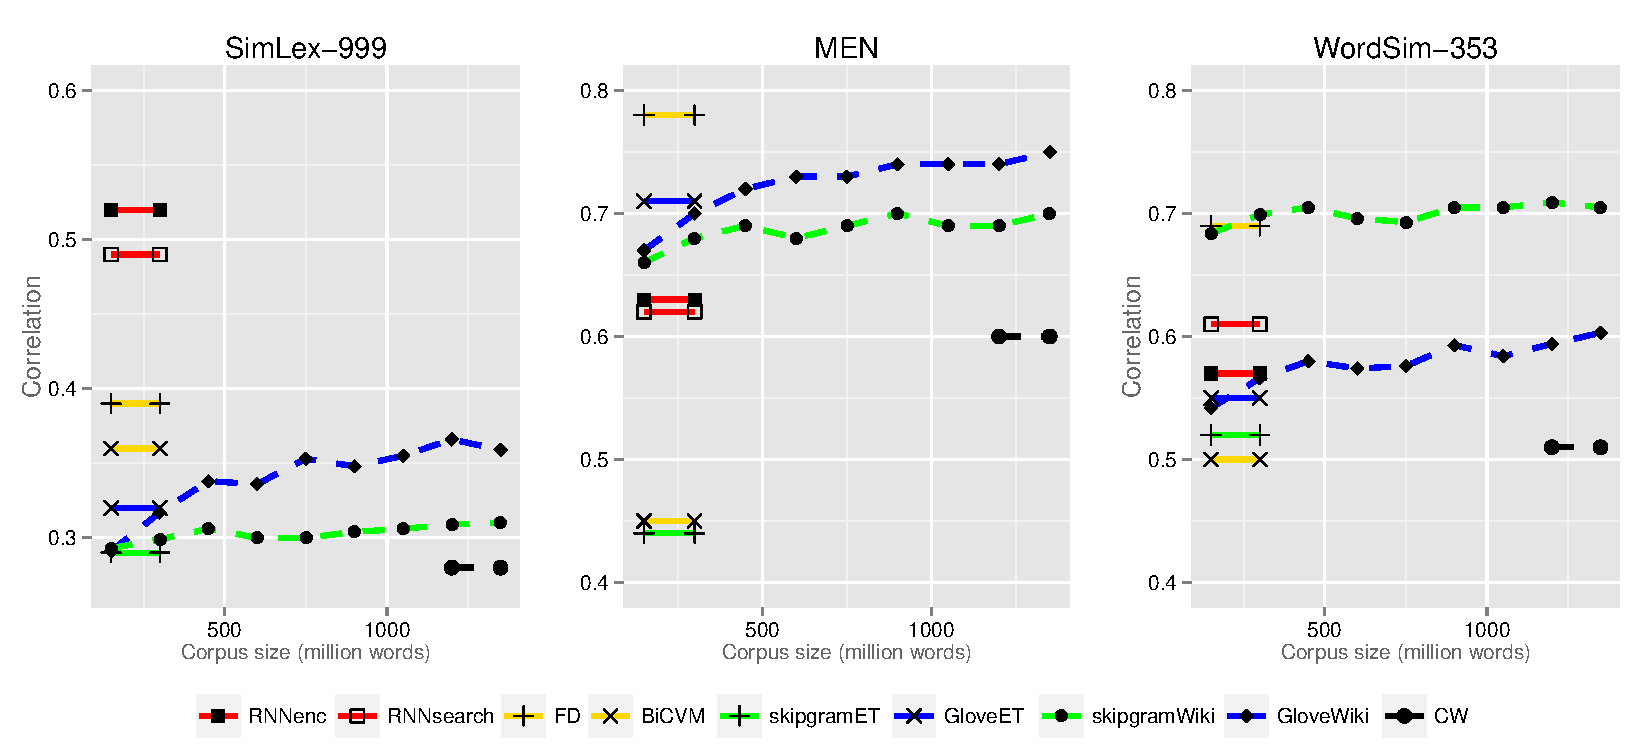
\includegraphics[width = \textwidth,clip=True,trim=0 10 0 10]{Chapter_3/Figure_1_ICLR2015}
\vspace{-4mm}
\caption{The effect of increasing the amount of training data on the quality of monolingual embeddings, based on similarity-based evaluations (SimLex-999) and two relatedness-based evaluations (MEN and WordSim-353). \emph{ET} in the legend indicates models trained on the English half of the translation corpus. \emph{Wiki} indicates models trained on Wikipedia.}
\label{fig:size}
\end{figure*}


\subsubsection{Analogy resolution}

Lexical analogy questions have been used as an alternative way of evaluating word representations. In this task, models must identify the correct answer (\emph{girl}) when presented with analogy questions such as `\emph{man} is to \emph{boy} as \emph{woman} is to ?'. It has been shown that Skipgram-style models are surprisingly effective at answering such questions~\citep{mikolov2013distributed}. This is because, if \( \bf m, b \) and \( \bf w\) are skigram-style embeddings for \emph{man}, \emph{boy} and \emph{woman} respectively, the correct answer is often the nearest neighbour in the vocabulary (by cosine distance) to the vector \( \bf v = w + b - m \). 

We evaluated embeddings on analogy questions using the same vector-algebra method as~\cite{mikolov2013distributed}. As in the previous section, for fair comparison I excluded questions containing a word outside the intersection of all model vocabularies, and restricted all answer searches to this reduced vocabulary. This left 11,166 analogies. Of these, 7219 are classed as `syntactic', in that they exemplify mappings between parts-of-speech or syntactic roles (e.g. \emph{fast} is to \emph{fastest} as \emph{heavy} is to \emph{heaviest}), and 3947 are classed as `semantic` (\emph{Ottawa} is to \emph{Canada} as \emph{Paris} is to \emph{France}), since successful answering seems to rely on some (world) knowledge of the concepts themselves. 

As shown in Fig.~\ref{fig:analogy}, NMT embeddings yield relatively poor answers to semantic analogy questions compared with monolingual embeddings and the bilingual embeddings \emph{FD} (which are projections of similar monolingual embeddings).\footnote{The performance of the FD embeddings on this task is higher than that reported by~\cite{faruqui2014improving} because I search for answers over a smaller total candidate vocabulary.} It appears that the translation objective prevents the embedding space from developing the same linear, geometric regularities as skipgram-style models with respect to semantic organisation. This also seems to be true of the embeddings from the full-sentence language model \emph{CW}. Further, in the case of the Glove and FD models this advantage seems to be independent of both the domain and size of the training data, since embeddings from these models trained on only the English half of the translation corpus still outperform the translation embeddings. 

On the other hand, NMT embeddings are effective for answering syntactic analogies using the vector algebra method. They perform comparably to or even better than monolingual embeddings when trained on less data (albeit bilingual data). It is perhaps unsurprising that the translation objective incentivises the encoding of a high degree of lexical syntactic information, since coherent target-language sentences could not be generated without knowledge of the parts-of-speech, tense or case of its vocabulary items. The connection between the translation objective and the embedding of lexical syntactic information is further supported by the fact that embeddings learned by the bilingual model BiCVM do not perform comparably on the syntactic analogy task. In this model, sentential semantics is transferred via a bag-of-words representation, presumably rendering the precise syntactic information less important.

When considering the two properties of NMT embeddings highlighted by these experiments, namely the encoding of semantic similarity and lexical syntax, it is worth noting that items in the similarity-focused evaluations of the previous section (SimLex-999 and TOEFL) consist of word groups or pairs that have identical syntactic role. Thus, even though lexical semantic information is in general pertinent to conceptual similarity~\citep{levy2014dependency}, the lexical syntactic and conceptual properties of translation embeddings are in some sense independent of one another.  


\begin{figure*}[ht]

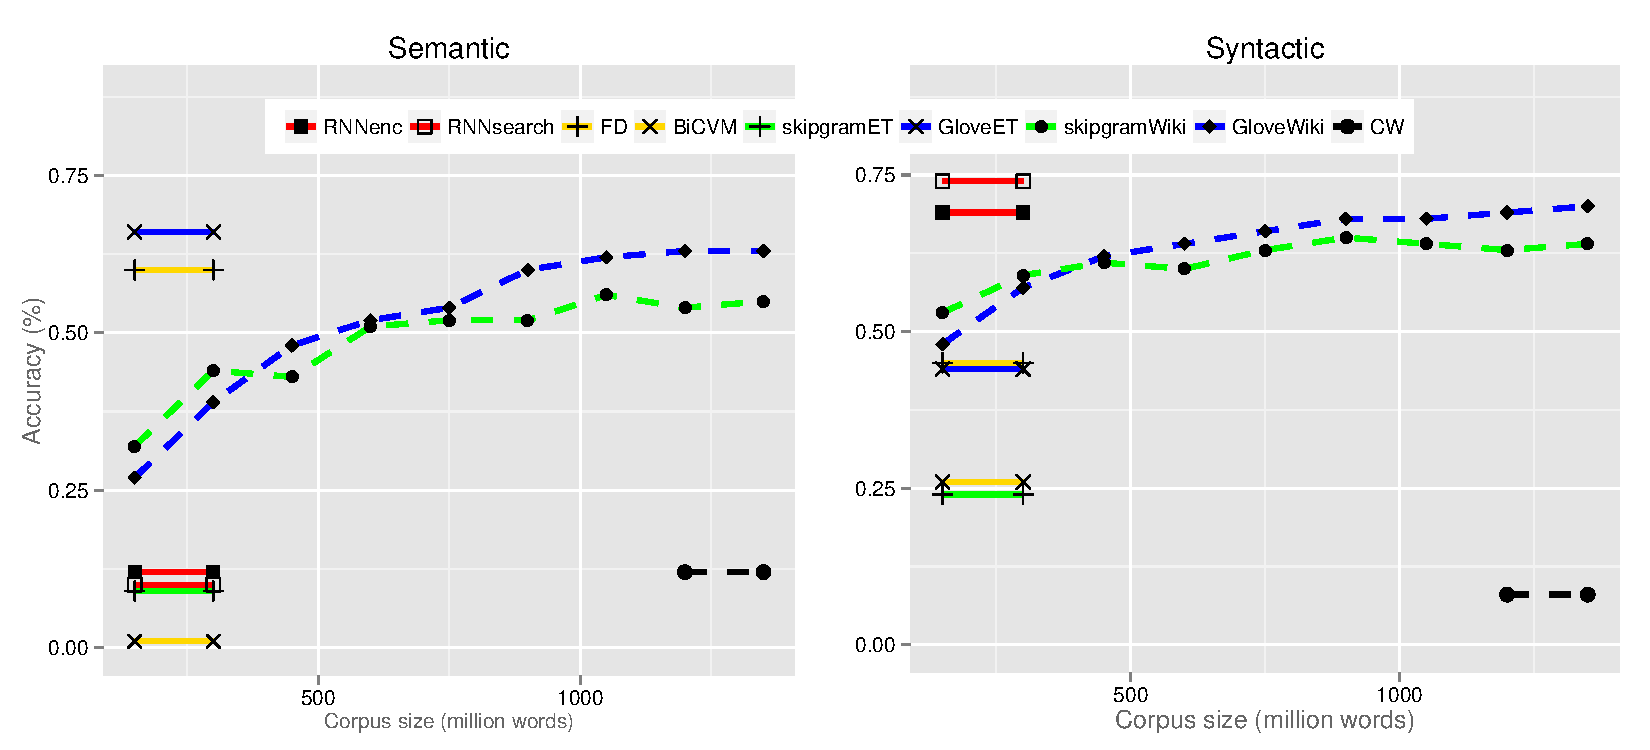
\includegraphics[width = \textwidth,clip=True,trim=0 10 0 10]{Chapter_3/Figure_2_ICLR2015}

\vspace{-4mm}
\caption{Translation-based embeddings perform best on syntactic analogies (\emph{run,ran: hide, hid}). Monolingual skipgram/Glove models are better at semantic analogies (\emph{father, man; mother, woman})}
\label{fig:analogy}

\end{figure*}

\section{Effect of Target Language}
\label{lang_effects}

To better understand why a translation objective yields embedding spaces with particular properties, I trained the RNN Search architecture to translate from English to German. 

\begin{table}[ht]
\small
\begin{center}
\begin{tabular}{r c | m{0.9cm}  m{0.9cm}  r c c c }


    \multicolumn{2}{c|}{~} &\bf  \small EN-FR &\bf  \small EN-DE &  &  `earned' & `castle' & `money'\\ 
\cline{1-4} \cline{6-8}
WordSim-353   & \(\rho\) & 0.60 & \bf 0.61 &   & {\small \emph{gained}} & {\small \emph{chateau}} & {\small \bf \emph{ silver}} \\
MEN & \(\rho\) & 0.61 & \bf 0.62 \bf & \bf \small  EN-FR  & {\small \bf \emph{won}} & {\small \emph{palace}} & {\small \emph{funds}} \\
SimLex-999 & \(\rho\) & 0.49 &  \bf 0.50 &  & {\small \emph{acquired}}  & {\small \emph{fortress}}  & {\small \emph{cash}} \\
\cline{6-8}
SimLex-Assoc-333 & \(\rho\) & 0.45  & \bf 0.47   &   &  &   \\
TOEFL & \(\%\) & 0.90 & \bf 0.93  & &  {\small \emph{gained}}&  {\small \emph{chateau}} &  {\small \emph{funds}} \\ 
Syn/antonym & \(\%\) & \bf 0.72 &  0.70  &  \bf \small EN-DE   &  {\small \emph{deserved}}    &  {\small \emph{palace}}    &  {\small \emph{cash}} \\ 
Syntactic analogies & \(\%\) & \bf 0.73 & 0.62   &  &  {\small \emph{accummulated}}   &  {\small \bf \emph{ padlock}}   &  {\small \emph{resources}} \\  
Semantic analogies & \(\%\) & 0.10 & \bf  0.11  \\
\end{tabular}
\caption{Comparison of embeddings learned by RNN Search models translating between English-French (EN-FR) and English-German (EN-DE) on all semantic evaluations (left) and nearest neighbours of selected cue words (right). Bold italics indicate target-language-specific effects. Evaluation items and vocabulary searches were restricted to words common to both models. }
\label{table:de}
\end{center}
\vspace{-5mm}
\end{table}

As shown in Table~\ref{table:de} (left side), the performance of the source (English) embeddings learned by this model was comparable to that of those learned by the English-to-French model on all evaluations, even though the English-German training corpus (91 million words) was notably smaller than the English-French corpus (348m words). This evidence shows that the desirable properties of translation embeddings highlighted thus far are not particular to English-French translation, and can also emerge when translating to a different language family, with different word ordering conventions.     

\subsection{Overcoming the vocabulary size problem}

A potential drawback to using NMT models for learning word embeddings is the computational cost of training such a model on large vocabularies. To generate a target language sentence, NMT models repeatedly compute a softmax distribution over the target vocabulary. This computation scales with vocabulary size and must be repeated for each word in the output sentence, so that training models with large output vocabularies is challenging. Moreover, while the same computational bottleneck does not apply to the encoding process or source vocabulary, there is no way in which a translation model could learn a high quality source embedding for a word if the plausible translations were outside its vocabulary. Thus, limitations on the size of the target vocabulary effectively limit the scope of NMT models as representation-learning tools. This contrasts with the shallower monolingual and bilingual representation-learning models considered in this paper,  which efficiently compute a distribution over a large target vocabulary using either a hierarchical softmax~\citep{morin2005hierarchical} or approximate methods such as negative sampling~\citep{mikolov2013distributed,Hermann:2014:ICLR}, and thus can learn large vocabularies of both source and target embeddings.

A recently proposed solution to this problem enables NMT models to be trained with larger target vocabularies (and hence larger meaningful source vocabularies) at comparable computational cost to training with a small target vocabulary~\citep{Jean}. The algorithm uses (biased) importance sampling~\citep{Bengio+Senecal-2003-small} to approximate the probability distribution of words over a large target vocabulary with a finite set of distributions over subsets of that vocabulary. Despite this element of approximation in the decoder, extending the effective target vocabulary in this way significantly improves translation performance, since the model can make sense of more sentences in the training data and encounters fewer unknown words at test time. In terms of representation learning, the method provides a means to scale up the NMT approach to vocabularies as large as those learned by monolingual models. However, given that the method replaces an exact calculation with an approximate one, I tested how the quality of source embeddings is affected by scaling up the target language vocabulary in this way. 

\begin{table}[t]
\small
\begin{center}
\begin{tabular}{r c | c c c c }
    \multicolumn{2}{c|}{~} &\bf RNN Search &\bf RNN Search & \bf RNN Search-LV  & \bf RNN Search-LV  \\ 
 \multicolumn{2}{c|}{~} &\bf \small EN-FR &\bf \small  EN-DE & \bf  \small EN-FR & \bf \small EN-DE \\ 
\hline
WordSim-353   & \(\rho\) & 0.60 & \bf 0.61 & 0.59 & 0.57  \\
MEN & \(\rho\) & 0.61 & \bf 0.62 & \bf 0.62 & 0.61 \\
SimLex-999 & \(\rho\) & 0.49 & 0.50 & \bf  0.51 & 0.50  \\
SimLex-Assoc-333 & \(\rho\) & 0.45  & \bf 0.47  & \bf 0.47  & 0.46   \\
TOEFL & \(\%\) & 0.90 & 0.93 & 0.93 & \bf 0.98  \\
Syn/antonym & \(\%\) & 0.72 &  0.70 & \bf 0.74 & 0.71 \\
Syntactic analogies & \(\%\) & \bf 0.73 &  0.62 & 0.71 & 0.62\\
Semantic analogies & \(\%\) & 0.10 &  0.11 & 0.08 & \bf 0.13\
\end{tabular}
\caption{Comparison of embeddings learned by the original (RNN Search - 30k French words, 50k German words) and extended-vocabulary (RNN Search-LV -500k words) models translating from English to French (EN-FR) and from English to German (EN-DE). For fair comparisons, all evaluations were restricted to the intersection of all model vocabularies.}
\label{table:ex}
\end{center}
\vspace{-5mm}
\end{table}

As shown in Table~\ref{table:ex}, there is no significant degradation of embedding quality when scaling to large vocabularies with using the approximate decoder. Note that for a fair comparison I filtered these evaluations to only include items that are present in the smaller vocabulary. Thus, the numbers do not directly reflect the quality of the additional 470k embeddings learned by the extended vocabulary models, which one would expect to be lower since they are words of lower frequency. All embeddings can be downloaded from \url{http://www.cl.cam.ac.uk/~fh295/}, and the embeddings from the smaller vocabulary models can be interrogated at \url{http://lisa.iro.umontreal.ca/mt-demo/embs/}.\footnote{A different solution to the rare-word problem was proposed by~\cite{luong2014addressing}. I do not evaluate the effects on the resulting embeddings of this method because I lack access to the source code.} 


\subsection{How similarity emerges in NMT embeddings}
\label{section:exp}

Although NMT models appear to encode both conceptual similarity and syntactic information for any source and target languages, it is not the case that embedding spaces will always be identical. Interrogating the nearest neighbours of the source embedding spaces of the English-French and English-German models reveals occasional language-specific effects. As shown in Table~\ref{table:de} (right side), the neighbours for the word \emph{earned} in the English-German model are as one might expect, whereas the neighbours from the English-French model contain the somewhat unlikely candidate \emph{won}. In a similar vein, while the neighbours of the word \emph{castle} from the English-French model are unarguably similar, the neighbours from the English-German model contain the word \emph{padlock}.
 
These infrequent but striking differences between the English-German and English-French source embedding spaces indicate how similarity might emerge effectively in NMT models. Tokens of the French verb \emph{gagner} have (at least) two possible English translations (\emph{win} and \emph{earn}). Since the translation model, which has limited encoding capacity, is trained to map tokens of \emph{win} and \emph{earn} to the same place in the target embedding space, it is efficient to move these concepts closer in the source space. Since \emph{win} and \emph{earn} map directly to two different verbs in German, this effect is not observed. On the other hand, the English nouns \emph{castle} and \emph{padlock} translate to a single noun (\emph{Schloss}) in German, but different nouns in French. Thus, \emph{padlock} and \emph{castle} are only close in the source embeddings from the English-German model. 

Based on these considerations, I can conjecture that the following condition on the semantic configuration between two language is crucial to the effective induction of lexical similarity. 

\MyQuote{\emph{For \(s_1\) and \(s_2\) in the source language, there is some \(t\) in the targThe horse raced past the barn fellet language such that there are sentences in the training data in which \(s_1\) translates to \(t\) and sentences in which \(s_2\) translates to \(t\).}}

{\centering \emph{if and only if} \\}

\MyQuote{\emph{\(s_1\) and \(s_2\) are semantically similar.}}

Of course, this condition is not true in general. However, I propose that the extent to which it holds over all possible word pairs corresponds to the quality of similarity induction in the translation embedding space. Note that strong polysemy in the target language, such as \emph{gagner = win, earn}, can lead to cases in which \(1\) is satisfied but \(2\) is not. The conjecture claims that these cases are detrimental to the quality of the embedding space (at least with regards to similarity). In practice, qualitative analyses of the embedding spaces and native speaker intuitions suggest that such cases are comparatively rare. Moreover, when such cases are observed, \(s_1\) and \(s_2\), while perhaps not similar, are not strongly dissimilar. This could explain why related but strongly dissimilar concepts such as antonym pairs do not converge in the translation embedding space. This is also consistent with qualitative evidence presented by~\cite{faruqui2014improving} that projecting monolingual embeddings into a bilingual space orientates them to better reflect the synonymy/antonymy distinction.
    

\subsection{Conclusions}

In this work, I have shown that the embedding spaces from neural machine translation models are orientated more towards conceptual similarity than those of monolingual models, and that translation embedding spaces also reflect richer lexical syntactic information. To perform well on similarity evaluations such as SimLex-999, embeddings must distinguish information pertinent to what concepts \emph{are} (their function or ontology) from information reflecting other non-specific inter-concept relationships. Concepts that are strongly related but dissimilar, such as antonyms, are particularly challenging in this regard~\citep{hill2014simlex}. Consistent with the qualitative observation made by~\cite{faruqui2014improving}, I suggested how the nature of the semantic correspondence between the words in languages enables NMT embeddings to distinguish synonyms and antonyms and, more generally, to encode the information needed to reflect human intuitions of similarity.   

The language-specific effects I observed in Section~\ref{lang_effects} suggest a potential avenue for improving translation and multi-lingual embeddings in future work. First, as the availability of fast GPUs for training grows, I would like to explore the embeddings learned by NMT models that translate between much more distant language pairs such as English-Chinese or English-Arabic. For these language pairs, the word alignment will less monotonic and may result in even more important semantic and syntactic information being encoded in the lexical representation. Further,  as observed by both~\cite{Hermann:2014:ICLR} and~\cite{faruqui2014improving}, the bilingual representation learning paradigm can be naturally extended to update representations based on correspondences between multiple languages (for instance by interleaving English-French and English-German training examples). Such an approach should smooth out language-specific effects, leaving embeddings that encode only language-agnostic conceptual semantics and are thus more generally applicable. Another related challenge is to develop smaller or less complex representation-learning tools that encode similarity with as much fidelity as NMT models but without the computational overhead. One promising approach for this is to learn word alignments and word embeddings jointly~\citep{Kocisky:2014}. This approach is effective for cross-lingual document classification, although the authors do evaluate the monolingual subspace induced by the model.

\section{Discussion}

Distributed word representations have been of interest to the NLP community for many years, but the emergence of neural language models has rendered them of interest to a far wider constituency of language engineers, machine learning researchers and artificial intelligence experts in general. The `embeddings' in NLMs have surprising and fundamental commonalities with distributed representations acquired by more traditional means. Nevertheless, there is something compelling about the way in which they `emerge' via the optimisation of cost functions corresponding (typically) to the sort of language prediction task that a lay human could easily describe or even attempt. This might lie behind their wide appeal.  

The single most important takeaway from this chapter is that not all sets of neural word embeddings are alike. In particular, their semantics depends in interesting ways on both the modality of the information to which the corresponding NLMs are exposed as well as its architecture and objective function. In the first section, I showed that the addition of information corresponding to the physical properties of concepts can enrich the quality of word embeddings. Moreover, while only concrete word concepts have such physical properties, in many cases, simple neural architectures like Skipgram are capable of propagating this information to a wider range of words that may have different parts-of-speech or refer to more abstract concepts. In the second section, I showed that NLMs whose objective is apparently more complex (translating sentences between languages) also acquire word embeddings with properties (semantic similarity) that are not observed so strongly in those trained via simpler objectives (neighbouring word prediction). Conveniently, it was evaluating with SimLex-999 that allowed this distinction to come to light (although it was corroborated via analyses on existing datasets such as the TOEFL synonymy questions). 




\chapter{Representing phrases with neural language models}
% This chapter is about phrase representations
\label{CH4}
\section{Introduction}

Much recent research in computational semantics has focussed on learning representations of arbitrary-length phrases and sentences. This task is challenging partly because there is no obvious gold standard of phrasal representation that could be used in training and evaluation. Consequently, it is difficult to design approaches that could learn from such a gold standard, and also hard to evaluate or compare different models.

In this work, we use dictionary definitions to address this issue. The composed meaning of the words in a dictionary definition (\emph{a tall, long-necked, spotted ruminant of Africa}) should correspond to the meaning of the word they define (\emph{giraffe}). This bridge between lexical and phrasal semantics is useful because high quality vector representations of single words can be used as a target when learning to combine the words into a coherent phrasal representation.
 
This approach still requires a model capable of learning to map between arbitrary-length phrases and fixed-length continuous-valued word vectors. For this purpose we experiment with two broad classes of neural language models (NLMs): Recurrent Neural Networks (RNNs), which naturally encode the order of input words, and simpler (feedforward) bag-of-words (BOW) embedding models. Prior to training these NLMs, we learn target lexical representations by training the Word2Vec software~\cite{mikolov2013distributed} on billions of words of raw text. 

We demonstrate the usefulness of our approach by building and releasing two applications. The first is a \emph{reverse dictionary} or \emph{concept finder}: a system that returns words based on user descriptions or definitions~\cite{zock2004word}. Reverse dictionaries are used by copywriters, novelists, translators and other professional writers to find words for notions or ideas that might be on the tip of their tongue. For instance, a travel-writer might look to enhance her prose by searching for examples of a \emph{country that people associate with warm weather} or \emph{an activity that is mentally or physically demanding}. We show that an NLM-based reverse dictionary trained on only a handful of dictionaries identifies novel definitions and concept descriptions comparably or better than commercial systems, which rely on significant task-specific engineering and access to much more dictionary data. Moreover, by exploiting models that learn bilingual word representations~\cite{307754,Klementiev,hermann2013multilingual,gouws2014bilbowa}, we show that the NLM approach can be easily extended to produce a potentially useful cross-lingual reverse dictionary.

The second application of our models is as a general-knowledge crossword question answerer. When trained on both dictionary definitions and the opening sentences of Wikipedia articles, NLMs produce plausible answers to (non-cryptic) crossword clues, even those that apparently require detailed world knowledge. Both BOW and RNN models can outperform bespoke commercial crossword solvers, particularly when clues contain a greater number of words. Qualitative analysis reveals that NLMs can learn to relate concepts that are not directly connected in the training data and can thus generalise well to unseen input. To facilitate further research, all of our code, training and evaluation sets (together with a system demo) are published online with this paper.\footnote{
    \url{https://www.cl.cam.ac.uk/~fh295/}
}

\section{Neural Language Model Architectures}

The first model we apply to the dictionary-based learning task is a recurrent neural network (RNN). RNNs operate on variable-length sequences of inputs; in our case, natural language definitions, descriptions or sentences. RNNs (with LSTMs) have achieved state-of-the-art performance in language modelling~\cite{mikolov2010recurrent}, image caption generation~\cite{kiros2014unifying} and approach state-of-the-art performance in machine translation~\cite{bahdanau2014neural}. 

During training, the input to the RNN is a dictionary definition or sentence from an encyclopedia. The objective of the model is to map these defining phrases or sentences to an embedding of the word that the definition defines. The target word embeddings are learned independently of the RNN weights, using the Word2Vec software~\cite{mikolov2013distributed}.   

The set of all words in the training data constitutes the vocabulary of the RNN. For each word in this vocabulary we randomly initialise a real-valued vector (input embedding) of model parameters. The RNN `reads' the first word in the input by applying a non-linear projection of its embedding \(v_1\) parameterised by input weight matrix \(W\) and \(b\), a vector of biases.
% Anna: the part below now appears in the the middle of the above sentence - force it to appear after.
\begin{align*}
A_1 = \phi( Wv_1 + b) 
\end{align*}
yielding the first internal activation state \(A_1\). In our implementation, we
use \(\phi(x) = \tanh(x)\), though in theory \(\phi\) can be any differentiable
non-linear function. Subsequent internal activations (after time-step \(t\))
are computed by projecting the embedding of the \(t^{th}\) word and using this
information to `update' the internal activation state. 
\begin{align*}
A_t =  \phi( UA_{t-1} + Wv_t + b ). 
\end{align*}

As such, the values of the final internal activation state units \(A_N\) are a
weighted function of all input word embeddings, and constitute a `summary' of
the information in the sentence.

\subsection{Long Short Term Memory}

A known limitation when training RNNs to read language using gradient descent is that the error signal (gradient) on the training examples either vanishes or explodes as the number of time steps (sentence length) increases \cite{bengio1994learning}. Consequently, after reading longer sentences the final internal activation \(A_N\) typically retains useful information about the most recently read (sentence-final) words, but can neglect important information near the start of the input sentence. LSTMs  \cite{hochreiter1997long} were designed to mitigate this long-term dependency problem. 

At each time step \(t\), in place of the single internal layer of units \(A\),
the LSTM RNN computes six internal layers \(i^w , g^i, g^f , g^o, h\) and
\(m\). The first, \(g^w\), represents the core information passed to the LSTM
unit by the latest input word at \(t\). It is computed as a simple linear
projection of the input embedding \(v_t\) (by input weights \(W_w\)) and the
\emph{output state} of the LSTM at the previous time step \(h_{t-1}\) (by
update weights \(U_w\)):
\begin{align*}
i_t^w = W_w v_t + U_wh_{t-1} +  b_w
\end{align*}

The layers \(g^i, g^f \) and \(g^o \) are computed as weighted sigmoid
functions of the input embeddings, again parameterised by layer-specific weight
matrices \(W\) and \(U\):
\begin{align*}
g_t^s = \frac{1}{1+\exp(-(W_s v_t + U_sh_{t-1} + b_s  ))}
\end{align*}
where \(s\) stands for one of \(i,f\) or \(o\). These vectors take
values on \([0,1]\) and are often referred to as \emph{gating activations}.
Finally, the \emph{internal memory state}, \(m_t\) and new output state
\(h_t\), of the LSTM at \(t\) are computed as
\begin{align*}
    m_t =& i_t^w \odot g_t^i + m_{t-1} \odot g_t^f \\
    h_t =& g_t^o \odot \phi(m_t), 
\end{align*}
where \(\odot\) indicates elementwise vector multiplication and \(\phi\) is, as
before, some non-linear function (we use \(tanh\)). Thus, \(g^i\) determines to
what extent the new \emph{input} word is considered at each time step, \(g^f\)
determines to what extent the existing state of the internal memory is retained
or \emph{forgotten} in computing the new internal memory, and \(g^o\)
determines how much this memory is considered when computing the output state
at \(t\). 

The sentence-final memory state of the LSTM, \(m_N\), a `summary' of all the
information in the sentence, is then projected via an extra non-linear
projection (parameterised by a further weight matrix) to a target embedding
space. This  layer enables the target (defined) word embedding space to take a
different dimension to the activation layers of the RNN, and in principle
enables a more complex definition-reading function to be learned. 

\subsection{Bag-of-Words NLMs}

We implement a simpler linear bag-of-words (BOW) architecture for encoding the
definition phrases. As with the RNN, this architecture learns an embedding
\(v_i\) for each word in the model vocabulary, together with a single matrix of
input projection weights \(W\). The BOW model simply maps an input definition
with word embeddings \(v_1 \dots v_n\) to the sum of the projected embeddings
\(\sum_{i=1}^n Wv_i \). This model can also be considered a special case of an
RNN in which the update function \(U\) and nonlinearity \(\phi\) are both the
identity, so that `reading' the next word in the input phrase updates the
current representation more simply:
\begin{align*}
A_t =  A_{t-1} + Wv_t.
\end{align*}

\subsection{Pre-trained Input Representations}

We experiment with variants of these models in which the input definition embeddings are pre-learned and fixed (rather than randomly-initialised and updated) during training. There are several potential advantages to taking this approach. First, the word embeddings are trained on massive corpora and may therefore introduce additional linguistic or conceptual knowledge to the models. Second, at test time, the models will have a larger effective vocabulary, since the pre-trained word embeddings typically span a larger vocabulary than the union of all dictionary definitions used to train the model. Finally, the models will then map to and from the same space of embeddings (the embedding space will be closed under the operation of the model), so conceivably could be more easily applied as a general-purpose `composition engine'.

\subsection{Training Objective}

We train all neural language models \(M\) to map the input definition phrase \(s_c\) defining word \(c\) to a location close to the the pre-trained embedding \(v_c\) of \(c\). We experiment with two different cost functions for the word-phrase pair \((c,s_c)\) from the training data. The first is simply the cosine distance between \(M(s_c)\) and \(v_c\). The second is the rank loss 
\[
\max(0, m - cos(M(s_c),v_c)-\cos(M(s_c),v_r))
\] 
where \(v_r\) is the embedding of a randomly-selected word from the vocabulary other than \(c\). This loss function was used for language models, for example, in~\cite{huang2012improving}. In all experiments we apply a margin \(m = 0.1\), which has been shown to work well on word-retrieval tasks~\cite{bordes2015large}. 

\subsection{Implementation Details}
Since training on the dictionary data took 6-10 hours, we did not conduct a hyper-parameter search on any validation sets over the space of possible model configurations such as embedding dimension, or size of hidden layers. Instead, we chose these parameters to be as standard as possible based on previous research. For fair comparison, any aspects of model design that are not specific to a particular class of model were kept constant across experiments. 

The pre-trained word embeddings used in all of our models (either as input or target) were learned by a continuous bag-of-words (CBOW) model using the Word2Vec software on approximately 8 billion words of running text.\footnote{The Word2Vec embedding models are well known; further details can be found at~\url{https://code.google.com/p/word2vec/} The training data for this pre-training was compiled from various online text sources using the script \emph{demo-train-big-model-v1.sh} from the same page.} When training such models on massive corpora, a large embedding length of up to 700 have been shown to yield best performance (see e.g.~\cite{faruqui2014retrofitting}). The pre-trained embeddings used in our models were of length 500, as a compromise between quality and memory constraints.

In cases where the word embeddings are learned during training on the dictionary objective, we make these embeddings shorter (256), since they must be learned from much less language data. In the RNN models, and at each time step each of the four LSTM RNN internal layers (gating and activation states) had length 512 -- another standard choice (see e.g.~\cite{cho2014learning}). The final hidden state was mapped linearly to length 500, the dimension of the target embedding. In the BOW models, the projection matrix projects input embeddings (either learned, of length 256, or pre-trained, of length 500) to length 500 for summing. 

All models were implemented with Theano~\cite{bergstra+al:2010-scipy} and trained with minibatch SGD on GPUs. The batch size was fixed at 16 and the learning rate was controlled by \emph{adadelta}~\cite{zeiler2012adadelta}. %We make all code for building and training the models publicly available.  

\section{Reverse Dictionaries}

The most immediate application of our trained models is as a \emph{reverse dictionary} or \emph{concept finder}. It is simple to look up a definition in a dictionary given a word, but professional writers often also require suitable words for a given idea, concept or definition.\footnote{See the testimony from professional writers at \url{http://www.onelook.com/?c=awards}} Reverse dictionaries satisfy this need by returning candidate words given a phrase, description or definition. For instance, when queried with the phrase \emph{an activity that requires strength and determination}, the OneLook.com reverse dictionary returns the concepts \emph{exercise} and \emph{work}. Our trained RNN model can perform a similar function, simply by mapping a phrase to a point in the target (Word2Vec) embedding space, and returning the words corresponding to the embeddings that are closest to that point.  

Several other academic studies have proposed reverse dictionary models. These generally rely on common techniques from information retrieval, comparing definitions in their internal database to the input query, and returning the word whose definition is `closest' to that query~\cite{bilac2003improving,bilac2004dictionary,zock2004word}. Proximity is quantified differently in each case, but is generally a function of hand-engineered features of the two sentences. For instance,~\cite{shaw2013building} propose a method in which the candidates for a given input query are all words in the model's database whose definitions contain one or more words from the query. This candidate list is then ranked according to a query-definition similarity metric based on the hypernym and hyponym relations in WordNet, features commonly used in IR such as \emph{tf-idf} and a parser. 

There are, in addition, at least two commercial online reverse dictionary applications, whose architecture is proprietary knowledge. The first is the Dictionary.com reverse dictionary \footnote{Available at \url{http://dictionary.reference.com/reverse/}}, which retrieves candidate words from the Dictionary.com dictionary based on user definitions or descriptions. The second is {\bf OneLook.com}, whose algorithm searches 1061 indexed dictionaries, including all major freely-available online dictionaries and resources such as Wikipedia and WordNet.

\subsection{Data Collection and Training}

To compile a bank of dictionary definitions for training the model, we started with all words in the target embedding space. For each of these words, we extracted dictionary-style definitions from five electronic resources: \emph{Wordnet, The American Heritage Dictionary, The Collaborative International Dictionary of English, Wiktionary} and \emph{Webster's}. We chose these five dictionaries because they are freely-available via the WordNik API,\footnote{See \url{http://developer.wordnik.com}} but in theory any dictionary could be chosen. Most words in our training data had multiple definitions. For each word \(w\) with definitions \( \{d_1 \dots d_n\} \) we included all pairs \((w, d_1) \dots (w,d_n) \) as training examples. 

To allow models access to more factual knowledge than might be present in a dictionary (for instance, information about specific entities, places or people, we supplemented this training data with information extracted from Simple Wikipedia.~\footnote{\url{https://simple.wikipedia.org/wiki/Main_Page}} For every word in the model's target embedding space that is also the title of a Wikipedia article, we treat the sentences in the first paragraph of the article as if they were (independent) definitions of that word. When a word in Wikipedia also occurs in one (or more) of the five training dictionaries, we simply add these pseudo-definitions to the training set of definitions for the word. Combining Wikipedia and dictionaries in this way resulted in \(\approx 900,000\) word-'definition' pairs of \(\approx 100,000\) unique words. 

To explore the effect of the quantity of training data on the performance of the models, we also trained models on subsets of this data. The first subset comprised only definitions from Wordnet (approximately 150,000 definitions of 75,000 words). The second subset comprised only words in Wordnet and their \emph{first} definitions (approximately 75,000 word, definition pairs).\footnote{As with other dictionaries, the first definition in WordNet generally corresponds to the most typical or common sense of a word.}. For all variants of RNN and BOW models, however, reducing the training data in this way resulted in a clear reduction in performance on all tasks. For brevity, we therefore do not present these results in what follows.  

\begin{table*}[ht]
    \centering
{\small
\hfill{}
\begin{tabular}{r|r|ccc|ccc|ccc|}

\multicolumn{2}{c}{}& \multicolumn{6}{|c|}{\bf Dictionary definitions} \\
\multicolumn{2}{c}{\textbf{Test Set }}&\multicolumn{3}{|c|}{\textbf{Seen} (500 WN defs)}& \multicolumn{3}{|c|}{\textbf{Unseen} (500 WN defs)} & \multicolumn{3}{|c|}{\textbf{Concept descriptions} (200)} \\

\hline

\rule{0pt}{2ex} 

Unsup. & W2V add & - & - & - & 923 & .04/.16 & 163 & 339 & .07/.30 & 150    \\
models  & W2V mult &- &- & -& 1000 & .00/.00 & 10* &   1000 & .00/.00 & 27* \\
\hdashline 
\rule{0pt}{2ex} 
& OneLook & \bf 0 & \bf .89/.91 & \bf 67  & - & - & - &  \bf 18.5 &  {\bf .38}/.58 & 153    \\
\hdashline 
\rule{0pt}{2ex} 
 & RNN cosine & 12 & .48/.73 & 103 &  22 & .41/.70 & 116 & 69 & .28/.54 & 157 \\
 & RNN w2v cosine & 19 & .44/.70 & 111 & 19 & .44/.69 & 126 & 26 & {\bf .38}/.66 & 111  \\
 & RNN ranking & 18 & .45/.67 & 128 &	24 & .43/.69 & 103 & 25 & .34/.66 & 102 \\
NLMs & RNN w2v ranking & 54 & .32/.56 & 155 & 33 & .36/.65 & 137 &	30 & .33/.69 & \bf 77 \\
& BOW cosine &22 & .44/.65 & 129 & 19 & .43/.69 & 103 & 50 & .34/.60 &  99 \\
& BOW w2v cosine & 15 & .46/.71 & 124 &  \bf14 & \bf .46/ .71 &  104	 & 28 & .36/.66 &  99 \\
& BOW ranking & 17 & .45/.68 &  115 &	 22 & .42/.70 & \bf 95 &	32 & .35/.69 & 101   \\
& BOW w2v rankng & 55 & .32/.56 & 155 &	36 & .35/.66 & 138 &	38 & .33/{\bf .72} & 85 \\

\hline 

\multicolumn{11}{c}{} \\
\multicolumn{5}{c}{}& \multicolumn{6}{|c|}{\emph{median rank \hspace{5mm}   accuracy@10/100 \hspace{5mm}   rank variance} } \\

\end{tabular}}
\caption{Performance of different reverse dictionary models in different evaluation settings. *Low variance in \emph{mult} models is due to consistently poor scores, so not highlighted.}
\label{results}
\end{table*}



\subsection{Comparisons}

As a baseline, we also implemented two entirely unsupervised methods using the neural (Word2Vec) word embeddings from the target word space. In the first ({\bf W2V add}), we compose the embeddings for each word in the input query by pointwise addition, and return as candidates the nearest word embeddings to the resulting composed vector.\footnote{Since we retrieve all answers from embedding spaces by cosine similarity, addition of word embeddings is equivalent to taking the mean.} The second baseline, ({\bf W2V mult}), is identical except that the embeddings are composed by elementwise multiplication. Both methods are established ways of building phrase representations from word embeddings~\cite{mitchell2010composition}.

None of the models or evaluations from previous academic research on reverse dictionaries is publicly available, so direct comparison is not possible. However, we do compare performance with the commercial systems. The Dictionary.com system returned no candidates for over 96\% of our input definitions. We therefore conduct detailed comparison with OneLook.com, which is the first reverse dictionary tool returned by a Google search and seems to be the most popular among writers. 

\subsection{Reverse Dictionary Evaluation}

To our knowledge there are no established means of measuring reverse dictionary performance. In the only previous academic research on English reverse dictionaries that we are aware of, evaluation was conducted on 300 word-definition pairs written by lexicographers~\cite{shaw2013building}. Since these are not publicly available we developed new evaluation sets and make them freely available for future evaluations.  

The evaluation items are of three types, designed to test different properties of the models. To create the {\bf seen} evaluation, we randomly selected 500 words from the WordNet training data (seen by all models), and then randomly selected a definition for each word. Testing models on the resulting 500 word-definition pairs assesses their ability to recall or decode previously encoded information. For the {\bf unseen} evaluation, we randomly selected 500 words from WordNet and excluded all definitions of these words from the training data of all models. 

Finally, for a fair comparison with OneLook, which has both the seen and unseen pairs in its internal database, we built a new dataset of {\bf concept descriptions} that do not appear in the training data for any model. To do so, we randomly selected 200 adjectives, nouns or verbs from among the top 3000 most frequent tokens in the British National Corpus~\cite{leech1994claws4} (but outside the top 100). We then asked ten native English speakers to write a single-sentence `description' of these words. To ensure the resulting descriptions were good quality, for each description we asked two participants who did not produce that description to list any words that fitted the description (up to a maximum of three). If the target word was not produced by one of the two checkers, the original participant was asked to re-write the description until the validation was passed.\footnote{Re-writing was required in 6 of the 200 cases.} These concept descriptions, together with other evaluation sets, can be downloaded from our website for future comparisons.

\begin{table}[ht]
{\small
\emph
\hfill{}
\begin{tabular}{r|cl}
\bf Test set & \bf Word & \bf Description \\
\hline
 Dictionary &   \emph{valve} & "control consisting of a mechanical   \\
definition  & & device for controlling fluid flow" \\ 
\rule{0pt}{2ex} 
Concept &   \emph{prefer} & "when you like one thing \\
description & & more than another thing" \\
\end{tabular}
\caption{Style difference between \emph{dictionary definitions} and \emph{concept descriptions} in the evaluation.}
\label{tb:tablename}}
\end{table}

Given a test description, definition, or question, all models produce a ranking of possible word answers based on the proximity of their representations of the input phrase and all possible output words. To quantify the quality of a given ranking, we report three statistics: the \emph{median rank} of the correct answer (over the whole test set, lower better), the proportion of training cases in which the correct answer appears in the top 10/100 in this ranking (\emph{accuracy@10/100} - higher better) and the variance of the rank of the correct answer across the test set (\emph{rank variance} - lower better). 

\subsection{Results}


Table~\ref{results} shows the performance of the different models in the three evaluation settings. Of the unsupervised composition models, elementwise addition is clearly more effective than multiplication, which almost never returns the correct word as the nearest neighbour of the composition. Overall, however, the supervised models (RNN, BOW and OneLook) clearly outperform these baselines. 

The results indicate interesting differences between the NLMs and the OneLook dictionary search engine. The Seen (WN first) definitions in Table~\ref{results} occur in both the training data for the NLMs and the lookup data for the OneLook model. Clearly the OneLook algorithm is better than NLMs at retrieving already available information (returning 89\% of  correct words among the top-ten candidates on this set). However, this is likely to come at the cost of a greater memory footprint, since the model requires access to its database of dictionaries at query time.\footnote{The trained neural language models are approximately half the size of the six training dictionaries stored as plain text, so would be hundreds of times smaller than the OneLook database of 1061 dictionaries if stored this way.}

The performance of the NLM embedding models on the (unseen) concept descriptions task shows that these models can generalise well to novel, unseen queries. While the median rank for OneLook on this evaluation is lower, the NLMs retrieve the correct answer in the top ten candidates approximately as frequently, within the top 100 candidates more frequently and with lower variance in ranking over the test set. Thus, NLMs seem to generalise more `consistenly' than OneLook on this dataset, in that they generally assign a reasonably high ranking to the correct word. In contrast, as can also be verified by querying our we demo, OneLook tends to perform either very well or poorly on a given query.\footnote{We also observed that the \emph{mean} ranking for NLMs was lower than for OneLook on the concept descriptions task.}

When comparing between NLMs, perhaps the most striking observation is that the RNN models do not significantly outperform the BOW models, even though the BOW model output is invariant to changes in the order of words in the definition. Users of the online demo can verify that the BOW models recover concepts from descriptions strikingly well, even when the words in the description are permuted. This observation underlines the importance of lexical semantics in the interpretation of language by NLMs, and is consistent with some other recent work on embedding sentences \cite{iyyer2015deep}.    

It is difficult to observe clear trends in the differences between NLMs that
learn input word embeddings and those with pre-trained (Word2Vec) input
embeddings. Both types of input yield good performance in some situations and
weaker performance in others. In general, pre-training input embeddings seems
to help most on the concept descriptions, which are furthest from the training
data in terms of linguistic style. This is perhaps unsurprising, since models
that learn input embeddings from the dictionary data acquire all of their
conceptual knowledge from this data (and thus may overfit to this setting),
whereas models with pre-trained embeddings have some semantic memory acquired
from general running-text language data and other knowledge acquired from the
dictionaries.

\begin{table*}[ht]
{\small
\emph
\hfill{}
\begin{tabular}{r|ccccc|}
\bf Input & \\
\bf Description & \bf OneLook & \bf W2V add &  \bf RNN  & \bf BOW \\
\hline

\rule{0pt}{3ex} 
%BOW model used: Wordnik_Wiki_feedforward_train.npz

  "a native of  & 1:\emph{country} 2:\emph{citizen} &  1:\emph{a} 2.\emph{the}   &  1:\emph{eskimo} 2:\emph{scandinavian}   &  1:\emph{frigid} 2:\emph{cold}    \\


a cold  & 3:\emph{foreign} 4:\emph{naturalize} &   3:\emph{another} 4:\emph{of}  & 3:\emph{arctic} 4:\emph{indian}  & 3:\emph{icy} 4:\emph{russian}\\
 country" & 5:\emph{cisco} &  5:\emph{whole} &  5:\emph{siberian}  &  5:\emph{indian} \\
\rule{0pt}{3ex} 
  "a way of & 1:\emph{drag} 2:\emph{whiz} &  1:\emph{the} 2:\emph{through}   &  1:\emph{glide} 2:\emph{scooting}  &  1:\emph{flying} 2:\emph{gliding} \\


moving  & 3:\emph{aerodynamics} 4:\emph{draught} &   3:\emph{a} 4:\emph{moving}  & 3:\emph{glides} 4:\emph{gliding}  & 3:\emph{glide} 4:\emph{fly}\\
 through & 5:\emph{coefficient of drag} &  5:\emph{in} &  5:\emph{flight} &  5:\emph{scooting}\\	
 the air"        & \\

\rule{0pt}{3ex} 
  "a habit that & 1:\emph{sisterinlaw} 2:\emph{fatherinlaw} &  1:\emph{annoy} 2:\emph{your}   &  1:\emph{bossiness} 2:\emph{jealousy} &  1:\emph{infidelity} 2:\emph{bossiness}  \\


might annoy & 3:\emph{motherinlaw} 4:\emph{stepson} &   3:\emph{might} 4:\emph{that}  & 3:\emph{annoyance} 4:\emph{rudeness} & 3:\emph{foible} 4:\emph{unfaithfulness}\\
 your spouse" & 5:\emph{stepchild} &  5:\emph{either} &  5:\emph{boorishness} &  5:\emph{adulterous} \\

\end{tabular}}
\hfill{}
\caption{The top-five candidates for example queries (invented by the authors) from different reverse dictionary models. Both the RNN and BOW models are without Word2Vec input and use the cosine loss.}
\label{qual}
\end{table*}

\subsection{Qualitative Analysis}

Some example output from the various models is presented in Table~\ref{qual}. The differences illustrated here are also evident from querying the web demo. The first example shows how the NLMs (BOW and RNN) generalise beyond their training data. Four of the top five responses could be classed as appropriate in that they refer to inhabitants of cold countries. However, inspecting the WordNik training data, there is no mention of \emph{cold} or anything to do with climate in the definitions of \emph{Eskimo}, \emph{Scandinavian}, \emph{Scandinavia} etc. Therefore, the embedding models must have learned that \emph{coldness} is a characteristic of Scandinavia, Siberia, Russia, relates to Eskimos etc. via connections with other concepts that are described or defined as \emph{cold}. In contrast, the candidates produced by the OneLook and (unsupervised) W2V baseline models have nothing to do with coldness.

The second example demonstrates how the NLMs generally return candidates whose linguistic or conceptual function is appropriate to the query. For a query referring explicitly to a means, method or process, the RNN and BOW models produce verbs in different forms or an appropriate deverbal noun. In contrast, OneLook returns words of all types (\emph{aerodynamics, draught}) that are arbitrarily related to the words in the query. A similar effect  is apparent in the third example. While the candidates produced by the OneLook model are the correct part of speech (Noun), and related to the query topic, they are not semantically appropriate. The dictionary embedding models are the only ones that return a list of plausible \emph{habits}, the class of noun requested by the input.  

  
\subsection{Cross-Lingual Reverse Dictionaries}

\begin{table*}[ht]
{\small
\emph
\hfill{}
\begin{tabular}{r|ccccc|}
\bf Input description & \bf RNN EN-FR & \bf W2V add &  \bf RNN + Google  \\
\hline
  "an emotion that you might feel & \emph{ \underline{triste}, \underline{pitoyable}} & \emph {insister, effectivement} & \emph{ sentiment, regretter} \\


after being rejected" & \emph{ \underline{r\'epugnante}, \underline{\'epouvantable}} & \emph{pourquoi, nous} &\emph{  \underline{peur, aversion} } \\
\rule{0pt}{3ex} 
"a small black flying insect that  & \emph{\underline{mouche}, canard} & \emph {attentivement, pouvions} & \emph{ voler, \underline{faucon}} \\ 
transmits disease and likes horses" &  \emph{  \underline{hirondelle}, pigeon} & \emph{pourrons, naturellement} & \emph{\underline{mouches}, volant} \\
\end{tabular}}
\hfill{}
\caption{Responses from cross-lingual reverse dictionary models to selected queries. Underlined responses are `correct' or potentially useful for a native French speaker.}
\label{cross}
\end{table*}


We now show how the RNN architecture can be easily modified to create a \emph{bilingual reverse dictionary} - a system that returns candidate words in one language given a description or definition in another. A bilingual reverse dictionary could have clear applications for translators or transcribers. Indeed, the problem of attaching appropriate words to concepts may be more common when searching for words in a  second language than in a monolingual context.  

To create the bilingual variant, we simply replace the Word2Vec target embeddings with those from a bilingual embedding space. Bilingual embedding models use bilingual corpora to learn a space of representations of the words in two languages, such that words from either language that have similar meanings are close together~\cite{hermann2013multilingual,lauly2014autoencoder,gouws2014bilbowa}. For a test-of-concept experiment, we used English-French embeddings learned by the state-of-the-art BilBOWA model~\cite{gouws2014bilbowa} from the Wikipedia (monolingual) and Europarl (bilingual) corpora.\footnote{The approach should work with any bilingual embeddings. We thank Stephan Gouws for doing the training.} We trained the RNN model to map from English definitions to English words in the bilingual space. At test time, after reading an English definition, we then simply return the nearest French word neighbours to that definition.  

Because no benchmarks exist for quantitative evaluation of bilingual reverse dictionaries, we compare this approach qualitatively with two alternative methods for mapping definitions to words across languages. The first is analogous to the W2V Add model of the previous section: in the bilingual embedding space, we first compose the embeddings of the English words in the query definition with elementwise addition, and then return the French word whose embedding is nearest to this vector sum. The second uses the RNN monolingual reverse dictionary model to identify an English word from an English definition, and then translates that word using Google Translate.

Table~\ref{cross} shows that the RNN model can be effectively modified to create a cross-lingual reverse dictionary. It is perhaps unsurprising that the W2V Add model candidates are generally the lowest in quality given the performance of the method in the monolingual setting. In comparing the two RNN-based methods, the RNN (embedding space) model appears to have two advantages over the RNN + Google approach. First, it does not require online access to a bilingual word-word mapping as defined e.g. by Google Translate. Second, it less prone to errors caused by word sense ambiguity. For example, in response to the query \emph{an emotion you feel after being rejected}, the bilingual embedding RNN returns emotions or adjectives describing mental states. In contrast, the monolingual+Google model incorrectly maps the plausible English response \emph{regret} to the verbal infinitive \emph{regretter}. The model makes the same error when responding to a description of a fly, returning the verb \emph{voler} (to fly). 


\subsection{Discussion}

We have shown that simply training RNN or BOW NLMs on six dictionaries yields a reverse dictionary that performs comparably to the leading commercial system, even with access to much less dictionary data. Indeed, the embedding models consistently return syntactically and semantically plausible responses, which are generally part of a more coherent and homogeneous set of candidates than those produced by the commercial systems. We also showed how the architecture can be easily extended to produce bilingual versions of the same model. 

In the analyses performed thus far, we only test the dictionary embedding approach on tasks that it was trained to accomplish
 (mapping definitions or descriptions to words). In the next section, we explore whether the knowledge learned by dictionary embedding models can be effectively transferred to a novel task. 

\section{General Knowledge (crossword) Question Answering}

The automatic answering of questions posed in natural language is a central problem of Artificial Intelligence. Although web search and IR techniques provide a means to find sites or documents related to language queries, at present, internet users requiring a specific fact must still sift through pages to locate the desired information. 

Systems that attempt to overcome this, via fully open-domain or general knowledge question-answering (open QA), generally require large teams of researchers, modular design and powerful infrastructure, exemplified by IBM's Watson~\cite{ferrucci2010building}. For this reason, much academic research focuses on settings in which the scope of the task is reduced. This has been achieved by restricting questions to a specific topic or domain~\cite{molla2007question}, allowing systems access to pre-specified passages of text from which the answer can be inferred~\cite{Iyyer:Boyd-Graber:Claudino:Socher:Daume-2014,weston2015towards}, or centering both questions and answers on a particular knowledge base~\cite{berant14paraphrasing,bordes2014question}. 

In what follows, we show that the dictionary embedding models introduced in the previous sections may form a useful component of an open QA system. Given the absence of a knowledge base or web-scale information in our architecture, we narrow the scope of the task by focusing on general knowledge crossword questions. General knowledge (non-cryptic, or quick) crosswords appear in national newspapers in many countries. Crossword question answering is more tractable than general open QA for two reasons. First, models know the length of the correct answer (in letters), reducing the search space. Second, some crossword questions mirror definitions, in that they refer to fundamental properties of concepts (\emph{a twelve-sided shape}) or request a category member (\emph{a city in Egypt}).\footnote{As our interest is in the language understanding, we do not address the question of fitting answers into a grid, which is the main concern of end-to-end automated crossword solvers~\cite{littman2002probabilistic}.} 

\subsection{Evaluation} 

General Knowledge crossword questions come in different styles and forms. We used the Eddie James crossword website to compile a bank of sentence-like general-knowledge questions.\footnote{\url{http://www.eddiejames.co.uk/}} Eddie James is one of the UK's leading crossword compilers, working for several national newspapers. Our { \bf long} question set consists of the first 150 questions (starting from puzzle \#1) from his general-knowledge crosswords, excluding clues of fewer than four words and those whose answer was not a single word (e.g. \emph{kingjames}).

To evaluate models on a different type of clue, we also compiled a set of {\bf short}er questions based on the Guardian Quick Crossword. Guardian questions still require general factual or linguistic knowledge, but are generally shorter and somewhat more cryptic than the longer Eddie James clues. We again formed a list of 150 questions, beginning on 1 January 2015 and excluding any questions with multiple-word answers. For clear contrast, we excluded those few questions of length greater than four words. Of these 150 clues, a subset of 30 were {\bf single-word} clues. All evaluation datasets are available online with the paper. 
% Anna: you mean with *this* paper?

As with the reverse dictionary experiments, candidates are extracted from models by inputting definitions and returning words corresponding to the closest embeddings in the target space. In this case, however, we only consider candidate words \emph{whose length matches the length specified in the clue}.

\begin{table}[ht]
{\small
\emph
\hfill{}
\begin{tabular}{r|cl}
\bf Test set & \bf Word & \bf Description \\
\hline

\hdashline
Long &   \emph{Baudelaire} & "French poet \\ 
 (150) & & and key figure \\ 
&& in the development \\ 
&& of Symbolism." \\
\hdashline 
\rule{0pt}{3ex} 

Short (120) &   \emph{satanist} & "devil devotee" \\

\hdashline
\rule{0pt}{3ex} 
Single-Word (30) &   \emph{guilt} & "culpability" \\
\end{tabular}
\caption{Examples of the different question types in the crossword question evaluation dataset.}
\label{tb:tablename}}
\end{table}

\begin{table*}[ht]
{\small
\hfill{}
\begin{tabular}{l|ccc|ccc|ccc|}
\multicolumn{1}{c}{} & \multicolumn{3}{c}{{\bf Question Type }}& \multicolumn{6}{|c|}{\emph{avg rank -accuracy@10/100 - rank variance} } \\
\multicolumn{10}{c}{} \\
\multicolumn{1}{c}{\textbf{}}&\multicolumn{3}{|c|}{\textbf{Long (150)}}& \multicolumn{3}{|c|}{\textbf{Short (120)}} & \multicolumn{3}{|c|}{\textbf{Single-Word (30)}}  \\
\hline
% OneLook & 137  & \bf .72/.86 & 111 & 132 & \bf .75/.88 & 108 & 106 & .73/.90 & 89 & 126 &  \bf .73/.8\\
One Across & & .39 / && & \bf .68 / &&& .70 / &  \\
Crossword Maestro& & .27 /&& & .43 /&&& .73 / & \\
\hdashline
W2V add & 42  & .31/.63 & 92  & 11 & .50/.78 & 66 & \bf 2 & \bf .79/.90 & 45  \\
\hdashline
RNN cosine	& 15 &  .43/.69 & 108 & 22 & .39/.67 & 117 & 72 & .31/.52 & 187 \\
RNN w2v cosine &	4 & .61/.82 & 60 & \bf 7 & .56/.79 & 60 & 12 & .48/.72 & 116 \\
RNN ranking 	& 6 & .58/.84 & \bf 48 & 10 & .51/.73 & 57 & 12 & .48/.69 & 67 \\
RNN w2v ranking &	\bf 3 & .62/.80 & 61 & 8 & .57/.78 & 49 & 12 & .48/.69 & 114 \\
BOW cosine & 4 & .60/.82 & 54 & \bf 7 & .56/.78 & 51 & 12 & .45/.72 & 137 \\
BOW w2v cosine & 4 & .60/.83 & 56 & \bf 7  & .54/.80 & 48 & 3 & .59/.79 & 111 \\
BOW ranking	& 5 & \bf .62/.87 & 50 & 8 & .58/\bf .83 & 37 & 8 & .55/.79 & \bf 39 \\
BOW w2v ranking & 5 & .60/.86 & \bf 48 & 8 & .56/.83 & \bf 35 & 4 & .55/.83 & 43 \\
\end{tabular}}
\hfill{}
\caption{Performance of different models on crossword questions of different length. The two commercial systems are evaluated via their web interface so only accuracy@10 can be reported in those cases. }
\label{results2}
\label{tb:tablename}
\end{table*}

\subsection{Benchmarks and Comparisons}

As with the reverse dictionary experiments, we compare RNN and BOW NLMs with a
simple unsupervised baseline of elementwise addition of Word2Vec vectors in the
embedding space (we discard the ineffective \emph{W2V mult} baseline), again
restricting candidates to words of the pre-specified length. We also compare to
two bespoke online crossword-solving engines. The first, One Across
(\url{http://www.oneacross.com/}) is the candidate generation module of the
award-winning \emph{Proverb} crossword system~\cite{littman2002probabilistic}.
Proverb, which was produced by academic researchers, has featured in national
media such as New Scientist, and beaten expert humans in crossword solving
tournaments. The second comparison is with Crossword Maestro
(\url{http://www.crosswordmaestro.com/}), a commercial crossword solving system
that handles both cryptic and non-cryptic crossword clues (we focus only on the
non-cryptic setting), and has also been featured in national
media.\footnote{
    See e.g.
    \url{http://www.theguardian.com/crosswords/crossword-blog/2012/mar/08/crossword-blog-computers-crack-cryptic-clues}
}
We are unable to compare against a third well-known automatic crossword solver,
\emph{Dr Fill}~\cite{ginsberg2011dr}, because code for Dr Fill's
candidate-generation module is not readily available. As with the RNN and
baseline models, when evaluating existing systems we discard candidates whose
length does not match the length specified in the clue.  

Certain principles connect the design of the existing commercial systems and differentiate them from our approach. Unlike the NLMs, they each require query-time access to large databases containing common crossword clues, dictionary definitions, the frequency with which words typically appear as crossword solutions and other hand-engineered and task-specific components~\cite{littman2002probabilistic,ginsberg2011dr}. 

\begin{table*}[ht]
{\small
\emph
\hfill{}
\begin{tabular}{r|ccccc|}
\bf Input Description & \bf One Across& \bf Crossword Maestro & \bf BOW &  \bf RNN  \\
\hline

\rule{0pt}{3ex} 

  "Swiss mountain & 1:\emph{noted} 2:\emph{front} & 1:\emph{after} 2:\emph{favor} & 1:\emph{\bf Eiger} 2.\emph{Crags}   &  1:\emph{\bf Eiger} 2:\emph{Aosta}  \\
peak famed for its & 3:\emph{\bf Eiger} 4:\emph{crown} & 3:\emph{ahead} 4:\emph{along} &   3:\emph{Teton} 4:\emph{Cerro}  & 3:\emph{Cuneo} 4:\emph{Lecco}\\
 north face (5)" & 5:\emph{fount} &  5:\emph{being} &  5:\emph{Jebel} &  5:\emph{Tyrol} \\
\rule{0pt}{3ex} 
  "Old Testament & 1:\emph{\bf Joshua} 2:\emph{Exodus} &  1:\emph{devise} 2:\emph{Daniel}& 1:\emph{Isaiah} 2:\emph{Elijah}   &  1:\emph{\bf Joshua} 2:\emph{Isaiah}  \\
successor to & 3:\emph{Hebrew} 4:\emph{person} &   3:\emph{Haggai} 4:\emph{ Isaiah}  &3:\emph{\bf Joshua} 4:\emph{Elisha}  & 3:\emph{Gideon} 4:\emph{Elijah}\\
 Moses (6)" & 5:\emph{across} & 5:\emph{Joseph}&  5:\emph{Yahweh} &  5:\emph{Yahweh} \\	
\rule{0pt}{3ex} 
  "The former & 1:\emph{Holland} 2:\emph{general} &  1:\emph{Holland} 2:\emph{ancient} & 1:\emph{\bf Guilder} 2:\emph{Holland}   &  1:\emph{\bf 	Guilder} 2:\emph{Escudos}  \\
currency of the  & 3:\emph{Lesotho} &   3:\emph{earlier} 4:\emph{onetime}&   3:\emph{Drenthe} 4:\emph{Utrecht}  & 3:\emph{Pesetas} 4:\emph{Someren}\\
 Netherlands&  &5:\emph{qondam}&  5:\emph{Naarden} &  5:\emph{Florins} \\
 (7)"&  \\
\rule{0pt}{3ex} 
  "Arnold, 20th & 1:\emph{surrealism} &  1:\emph{disharmony}  & 1:\emph{\bf Schoenberg}   &  1:\emph{Mendelsohn} \\
Century composer &  2:\emph{laborparty}  &   2:\emph{dissonance} &  2:\emph{Christleib}  &  2:\emph{Williamson}  \\
pioneer of &  3:\emph{tonemusics}  &  3:\emph{bringabout} &  3:\emph{Stravinsky}  &  3:\emph{Huddleston}   \\
 atonality &4:\emph{introduced}  & 4:\emph{constitute} &4:\emph{Elderfield} & 4:\emph{Mandelbaum} \\
(10)"& 5:\emph{\bf Schoenberg} & 5:\emph{triggeroff} & 5:\emph{Mendelsohn} &  5:\emph{Zimmerman}\\

\end{tabular}}
\hfill{}
\caption{Responses from different models to example crossword clues. In each case the model output is filtered to exclude any candidates that are not of the same length as the correct answer. BOW and RNN models are trained without Word2Vec input embeddings and cosine loss.}
\label{egs}
\end{table*}

\subsection{Results}

The performance of models on the various question types is presented in Table~\ref{results2}. When evaluating the two commercial systems, One Across and Crossword Maestro, we have access to web interfaces that return up to approximately 100 candidates for each query, so can only reliably record membership of the top ten (accuracy@10).

On the long questions, we observe a clear advantage for all dictionary embedding models over the commercial systems and the simple unsupervised baseline. Here, the best performing NLM (RNN with Word2Vec input embeddings and ranking loss) ranks the correct answer third on average, and in the top-ten candidates over 60\% of the time.
	
As the questions get shorter, the advantage of the embedding models diminishes. Both the unsupervised baseline and One Across answer the short questions with comparable accuracy to the RNN and BOW models. One reason for this may be the difference in form and style between the shorter clues and the full definitions or encyclopedia sentences in the dictionary training data. As the length of the clue decreases, finding the answer often reduces to generating synonyms (\emph{culpability - guilt}), or category members (\emph{tall animal - giraffe}). The commercial systems can retrieve good candidates for such clues among their databases of entities, relationships and common crossword answers. Unsupervised Word2Vec representations are also  known to encode these sorts of relationships (even after elementwise addition for short sequences of words)~\cite{mikolov2013distributed}. This would also explain why the dictionary embedding models with pre-trained (Word2Vec) input embeddings outperfom those with learned embeddings, particularly for the shortest questions. 


\subsection{Qualitative Analysis}

A better understanding of how the different models arrive at their answers can be gained from considering specific examples, as presented in Table~\ref{egs}. The first three examples show that, despite the apparently superficial nature of its training data (definitions and introductory sentences) embedding models can answer questions that require factual knowledge about people and places. Another notable characteristic of these model is the consistent semantic appropriateness of the candidate set. In the first case, the top five candidates are all mountains, valleys or places in the Alps; in the second, they are all biblical names. In the third, the RNN model retrieves currencies, in this case performing better than the BOW model, which retrieves entities of various type associated with the Netherlands. Generally speaking (as can be observed by the web demo), the `smoothness' or consistency in candidate generation of  the dictionary embedding models is greater than that of the commercial systems. Despite its simplicity, the unsupervised W2V addition method is at times also surprisingly effective, as shown by the fact that it returns \emph{Joshua} in its top candidates for the third query.

The final example in Table~\ref{egs} illustrates the surprising power of the BOW model. In the training data there is a single definition for the correct answer \emph{Schoenberg}: \emph{United States composer and musical theorist (born in Austria) who developed atonal composition}. The only word common to both the query and the definition is 'composer' (there is no tokenization that allows the BOW model to directly connect \emph{atonal} and \emph{atonality}). Nevertheless, the model is able to infer the necessary connections between the concepts in the query and the definition to return Schoenberg as the top candidate. 

Despite such cases, it remains an open question whether, with more diverse training data, the world knowledge required for full open QA (e.g. secondary facts about \emph{Schoenberg}, such as his family) could be encoded and retained as weights in a (larger) dynamic network, or whether it will be necessary to combine the RNN with an external memory that is less frequently (or never) updated. This latter approach has begun to achieve impressive results on certain QA and entailment tasks~\cite{bordes2014question,graves2014neural,weston2015towards}.   


\section{Conclusion}

Dictionaries exist in many of the world's languages. We have shown how these lexical resources can constitute valuable data for training the latest neural language models to interpret and represent the meaning of phrases and sentences. While humans use the phrasal definitions in dictionaries to better understand the meaning of words, machines can use the words to better understand the phrases. We used two dictionary embedding architectures - a recurrent neural network architecture with a long-short-term memory, and a simpler linear bag-of-words model - to explicitly exploit this idea. 

On the reverse dictionary task that mirrors its training setting, NLMs that embed all known concepts in a continuous-valued vector space perform comparably to the best known commercial applications despite having access to many fewer definitions. Moreover, they generate smoother sets of candidates and require no linguistic pre-processing or task-specific engineering. We also showed how the description-to-word objective can be used to train models useful for other tasks. NLMs trained on the same data can answer general-knowledge crossword questions, and indeed outperform commercial systems on questions containing more than four words. While our QA experiments focused on crosswords, the results suggest that a similar embedding-based approach may ultimately lead to improved output from more general QA and dialog systems and information retrieval engines in general.  

We make all code, training data, evaluation sets and both of our linguistic tools publicly available online for future research. In particular, we propose the reverse dictionary task as a comparatively general-purpose and objective way of evaluating how well models compose lexical meaning into phrase or sentence representations (whether or not they involve training on definitions directly). 

In the next stage of this research, we will explore ways to enhance the NLMs described here, especially in the question-answering context. The models are currently not trained on any question-like language, and would conceivably improve on exposure to such linguistic forms. We would also like to understand better how BOW models can perform so well with no `awareness' of word order, and whether there are specific linguistic contexts in which models like RNNs or others with the power to encode word order are indeed necessary. Finally, we intend to explore ways to endow the model with richer world knowledge. This may require the integration of an external memory module, similar to the promising approaches proposed in several recent papers~\cite{graves2014neural,weston2015towards}.

\chapter{Representing sentences with neural language models}
% This chapter is about sentence representations
\label{CH5}

Distributed representations - dense real-valued vectors that encode the semantics of linguistic units - are ubiquitous in today's NLP research. As detailed in Chapters~\ref{CH2} and~\ref{CH3}, there are established ways to acquire such representations from naturally occurring (unlabelled) training data based on comparatively task-agnostic objectives (such as predicting adjacent words). Such methods are well understood empirically \citep{baroni2014don} and theoretically \citep{levy2014neural}. The best word representation spaces reflect consistently-observed aspects of human conceptual organisation~\citep{hill2014simlex}, and can be added as features to improve the performance of numerous language processing systems \citep{collobert2011natural}. 

As suggested in Chapter~\ref{CH4}, the task of learning such representations for longer linguistic units such as phrases or sentences is far harder, and there is comparatively little consensus on the best ways to attack this problem.\footnote{See the contrasting conclusions in \citep{mitchell2008vector,clark2007combining,baroni2014frege,milajevs2014evaluating} among others.} Nevertheless, with the advent of deeper language processing techniques, a class of neural language models has emerged that do indeed compute internal representations of phrases or sentences as continuous-valued vectors. Examples include machine translation~\citep{Sutskever2014sequence}, image captioning \citep{mao2014deep} and dialogue systems~\citep{serban2015building}. While it has been observed informally that the internal sentence representations of these models can reflect some semantic intuitions~\citep{cho2014learning}, it is not known which architectures or objectives yield the `best' or most useful representations. Resolving this question could ultimately have a significant impact on language processing systems. Indeed, it is phrases and sentences, rather than individual words, that encode the human-like general world knowledge (or `common sense')~\citep{norman1972memory} that is a critical missing part of most current language understanding systems.

In this chapter, I address these questions with a systematic comparison of the distributed phrase and sentence representations acquired by cutting-edge NLMs. I focus on methods that do not require labelled data gathered for the purpose of training models, since such methods are more cost-effective and applicable across languages and domains. I also propose two new phrase or sentence representation learning objectives - \emph{Sequential Denoising Autoencoders} (SDAEs) and \emph{FastSent}, a sentence-level log-linear bag-of-words model. I compare all methods on two types of task - \emph{supervised} and \emph{unsupervised evaluations} - reflecting different ways in which representations are ultimately to be used. In the former setting, a classifier or regression model is applied to representations and trained with task-specific labelled data, while in the latter, representation spaces are directly queried using cosine distance.    

I observe notable differences in approaches depending on the nature of the evaluation metric. In particular, deeper or more complex models (which require greater time and resources to train) generally perform best in the supervised setting, whereas shallow log-linear models work best on unsupervised benchmarks. Specifically, SkipThought Vectors~\citep{kiros2015skip} perform best on the majority of supervised evaluations, but SDAEs are the top performer on paraphrase identification. In contrast, on the (unsupervised) SICK sentence relatedness benchmark, FastSent, a simple, log-linear variant of the SkipThought objective, performs better than all other models. Interestingly, the method that exhibits strongest performance across both supervised and unsupervised benchmarks is a bag-of-words model trained to compose word embeddings using dictionary definitions~\citep{hill2015learning}. Taken together, these findings constitute valuable guidelines for the application of phrasal or sentential representation-learning to language understanding systems.

\section{Distributed Sentence Representations}

To constrain the analysis, I compare neural language models that compute sentence representations from unlabelled, naturally-ocurring data, as with the predominant methods for word representations.\footnote{This excludes innovative supervised sentence-level architectures including those of \cite{socher2011semi},\cite{kalchbrenner2014convolutional} and many others.} Likewise, I do not focus on `bottom up' models where phrase or sentence representations are built from fixed mathematical operations on word vectors (although I do consider a canonical case - see CBOW below); these were already compared by~\cite{milajevs2014evaluating}. Most space is devoted to the novel approaches, and I refer the reader to the original papers for more details of existing models. 

\subsection{Existing Models Trained on Text}
{\bf SkipThought Vectors} For consecutive sentences \(S_{i-1},S_i,S_{i+1}\) in some document, the {\bf SkipThought} model \citep{kiros2015skip} is trained to predict target sentences \(S_{i-1}\) and \(S_{i+1}\) given source sentence \(S_i\). As with all~\emph{sequence-to-sequence} models, in training the source sentence is `encoded' by a Recurrent Neural Network (RNN) (with Gated Recurrent Units~\citep{cho2014learning}) and then `decoded' into the two target sentences in turn. Importantly, because RNNs employ a single set of update weights at each time-step, both the encoder and decoder are sensitive to the order of words in the source sentence. 

For each position in a target sentence \(S_t\), the decoder computes a softmax distribution over the model's vocabulary. The cost of a training example is the sum of the negative log-likelihood of each correct word in the target sentences \(S_{i-1}\) and \(S_{i+1}\). This cost is backpropagated to train the encoder (and decoder), which, when trained, can map sequences of words to a single vector.

\vspace{5pt}\noindent {\bf ParagraphVector} \cite{le2014distributed} proposed two log-linear models of sentence representation. The {\bf DBOW} model learns a vector \(\mathbf{s}\) for every sentence \(S\) in the training corpus which, together with word embeddings \(v_w\), define a softmax distribution optimised to predict words \(w \in S\) given \(S\). The \(v_w\) are shared across all sentences in the corpus. In the {\bf DM} model, \(k\)-grams of consecutive words \(\{w_i \dots w_{i+k} \in S\}\) are selected and \(\mathbf{s}\) is combined with \(\{v_{w_i} \dots v_{w_{i+k}} \}\) to make a softmax prediction (parameterised by additional weights) of \(w_{i+k+1}\). 

I used the Gensim implementation,\footnote{\scriptsize \url{https://radimrehurek.com/gensim/}} treating each sentence in the training data as a `paragraph' as suggested by the authors. During training, both DM and DBOW models store representations for every sentence (as well as word) in the training corpus. Even on large servers it was therefore only possible to train models with representation size \(200\), and DM models whose combination operation was averaging (rather than concatenation). 

\vspace{5pt}\noindent{\bf Bottom-Up Methods} I train {\bf CBOW} and {\bf SkipGram} word embeddings \citep{mikolov2013distributed} on the Books corpus, and compose by elementwise addition as proposed by \cite{mitchell2010composition}.\footnote{I also tried multiplication but this gave very poor results.} 

I also compare to {\bf C-PHRASE}~\citep{marcobaronijointly}, an approach that exploits a (supervised) parser to infer distributed semantic representations based on a syntactic parse of sentences. C-PHRASE achieves state-of-the-art results for distributed representations on several evaluations used in this study.\footnote{Since code for C-PHRASE is not publicly-available I use the available pre-trained model ({\scriptsize \url{http://clic.cimec.unitn.it/composes/cphrase-vectors.html}}). Note this model is trained on \(3\times\) more text than others in this study.}

\vspace{5pt}\noindent{\bf Non-Distributed Baseline} I implement a {\bf TFIDF BOW} model in which the representation of sentence \(S\) encodes the count in \(S\) of a set of feature-words weighted by their \emph{tfidf} in \(C\), the corpus. The feature-words are the 200,000 most common words in \(C\). 

\subsection{Models Trained on Structured Resources}
The following models rely on (freely-available) data that has more structure than raw text.

\vspace{5pt}\noindent{\bf DictRep} \cite{hill2015learning} trained neural language models to map dictionary definitions to pre-trained word embeddings of the words defined by those definitions. They experimented with {\bf BOW} and {\bf RNN} (with LSTM) encoding architectures and variants in which the input word embeddings were either learned or pre-trained ({\bf+embs.}) to match the target word embeddings. I implement their models using the available code and training data.\footnote{{\scriptsize \url{https://www.cl.cam.ac.uk/~fh295/}}. Definitions from the training data matching those in the WordNet STS 2014 evaluation (used in this study) were excluded.}

\vspace{5pt}\noindent{\bf CaptionRep} Using the same overall architecture, I trained ({\bf BOW} and {\bf RNN}) models to map captions in the COCO dataset~\citep{chen2015microsoft} to pre-trained vector representations of images. The image representations were encoded by a deep convolutional network \citep{szegedy2014going} trained on the ILSVRC 2014 object recognition task \citep{russakovsky2014imagenet}. Multi-modal distributed representations can be encoded by feeding test sentences forward through the trained model. 

\vspace{5pt}\noindent{\bf NMT} I consider the sentence representations learned by neural MT models. These models have identical architecture to SkipThought, but are trained on sentence-aligned translated texts. I used a standard architecture \citep{cho2014learning} on all available {\bf En-Fr} and {\bf En-De} data from the 2015 Workshop on Statistical MT (WMT).\footnote{\scriptsize \url{www.statmt.org/wmt15/translation-task.html}} 

\subsection{Novel Text-Based Models}
I introduce two new approaches designed to address certain limitations with the existing models.

\vspace{5pt}\noindent{\bf Sequential (Denoising) Autoencoders} The SkipThought objective requires training text with a coherent inter-sentence narrative, making it problematic to port to domains such as social media or artificial language generated from symbolic knowledge. To avoid this restriction, I experiment with a representation-learning objective based on \emph{denoising autoencoders} (DAEs). In a DAE, high-dimensional input data is corrupted according to some noise function, and the model is trained to recover the original data from the corrupted version. As a result of this process, DAEs learn to represent the data in terms of features that explain its important factors of variation~\citep{vincent2008extracting}. Transforming data into DAE representations (as a `pre-training' or initialisation step) gives more robust (supervised) classification performance in deep feedforward networks \citep{vincent2010stacked}.

The original DAEs were feedforward nets applied to (image) data of fixed size. Here, I adapt the approach to variable-length sentences by means of a noise function \(N(S | p_o,p_x)\), determined by free parameters \(p_o,p_x \in [0,1]\). First, for each word \(w\) in \(S\), \(N\) deletes \(w\) with (independent) probability \(p_o\). Then, for each non-overlapping bigram \(w_i w_{i+1}\) in \(S\), \(N\) swaps \(w_i\) and \(w_{i+1}\) with probability \(p_x\). I then train the same LSTM-based encoder-decoder architecture as NMT, but with the denoising objective to predict (as target) the original source sentence \(S\) given a corrupted version \(N(S |p_o,p_x)\) (as source). The trained model can then encode novel word sequences into distributed representations. I call this model the \emph{Sequential Denoising Autoencoder} ({\bf SDAE}). Note that, unlike SkipThought, SDAEs can be trained on sets of sentences in arbitrary order.   

I label the case with no noise (i.e. \(p_o = p_x = 0\) and \(N \equiv id\)) {\bf SAE}. This setting matches the method applied to text classification tasks by \cite{dai2015semi}. The `word dropout' effect when \(p_o \geq 0\) has also been used as a regulariser for deep nets in supervised language tasks \citep{iyyer2015deep}, and for large \(p_x\) the objective is similar to word-level `debagging'~\citep{sutskever2011generating}. For the SDAE, I tuned \(p_o\), \(p_x\) on the validation set (see Section~\ref{unseval}).\footnote{I searched \(p_o,p_x \in \{0.1,0.2,0.3\}\) and observed best results with \(p_o = p_x = 0.1\).} I also tried a variant ({\bf +embs}) in which words are represented by (fixed) pre-trained embeddings. 

\vspace{5pt}\noindent{\bf FastSent} The performance of SkipThought vectors shows that rich sentence semantics can be inferred from the content of adjacent sentences. The model could be said to exploit a type of \emph{sentence-level Distributional Hypothesis}~\citep{harris1954distributional,polajnar2015exploration}. Nevertheless, like many deep neural language models, SkipThought is very slow to train (see Table~\ref{modelprops}). FastSent is a simple additive (log-linear) sentence model designed to exploit the same signal, but at much lower computational expense. Given a BOW representation of some sentence in context, the model simply predicts adjacent sentences (also represented as BOW) .

More formally, FastSent learns a source \(u_w\) and target \(v_w\) embedding for each word in the model vocabulary. For a training example  \(S_{i-1},S_i,S_{i+1}\) of consecutive sentences, \(S_i\) is represented as the sum of its source embeddings \( \mathbf{s_i} = \sum_{w \in S_i} u_w \). The cost of the example is then simply:
\begin{equation} \label{eqn1}
 \sum_{w \in S_{i-1} \cup S_{i+1}} \phi(\mathbf{s_i},v_w) 
 \end{equation}
 where \( \phi(v_1,v_2) \) is the softmax function.  

I also experiment with a variant ({\bf+AE}) in which the encoded (source) representation must predict its own words as target in addition to those of adjacent sentences. Thus in FastSent+AE, (\ref{eqn1}) becomes  \begin{equation} 
\sum_{w \in S_{i-1} \cup S_{i} \cup S_{i+1}} \phi(\mathbf{s_i},v_w).
\end{equation}

\noindent At test time the trained model (very quickly) encodes unseen word sequences into distributed representations with \( \mathbf{s} = \sum_{w \in S} u_w \).

\begin{table}
\centering 

    \begin{tabular}{l|ccccccc}\\
         & \rot{OS} & \rot{R} & \rot{WO} & \rot{SD} & \rot{WD}
        & \rot{TR} & \rot{TE} \\
        \cmidrule{1-8}
        S(D)AE              & & & \OK  & 2400 & 100 & 72* &  640 \\
        ParagraphVec &  & &   & 100 & 100&  4 & 1130  \\
        CBOW                &&  &   &  500 & 500 &  2 & 145  \\
        SkipThought             & \OK &  & \OK  & 4800 & 620 & 336* & 890  \\
        FastSent               & \OK &  & & 100 & 100 & 2  & 140  \\
        DictRep                & &  \OK & \OK  & 500 & 256 & 24* & 470  \\
        CaptionRep                & & \OK  & \OK  & 500 &  256 & 24* & 470  \\
        NMT                & & \OK & \OK  &  2400 & 512 &  72* & 720  \\
        \cmidrule[1pt]{1-8}
    \end{tabular}
    \caption{\label{modelprops} {\bf Properties of models compared in this study} \hspace{6mm} {\bf OS:} requires training corpus of sentences in order. {\bf R:} requires structured resource for training. {\bf WO:} encoder sensitive to word order. {\bf SD:} dimension of sentence representation. {\bf WD:} dimension of word representation. {\bf TR:} approximate training time (hours) on the dataset in this paper. * indicates trained on GPU. {\bf TE:} approximate time (s) taken to encode 0.5m sentences.}

\end{table}
\begin{table*}[ht]
\begin{adjustwidth}{-1.6cm}{}
\renewcommand{\tabcolsep}{4.6pt}
\footnotesize
\newcommand{\mc}[1]{\multicolumn{1}{l|}{#1}}
  \begin{center}

      {
        \begin{tabular}{rr|l|l|c}
          \multicolumn{2}{c|}{Dataset} & \multicolumn{1}{c}{Sentence 1} &\multicolumn{1}{|c|}{Sentence 2} & \(/5\)  \\
          \hline
          \hline
           & News & \emph{Mexico wishes to guarantee citizens' safety.} &\emph{Mexico wishes to avoid more violence.} & 4 \\
           & Forum &  \emph{The problem is simpler than that.} &  \emph{The problem is simple.}  & 3.8 \\
           STS & WordNet &  \emph{A social set or clique of friends.} &  \emph{An unofficial association of people or groups.} & 3.6 \\
           2014 & Twitter & \emph{Taking Aim  \#Stopgunviolence \#Congress \#NRA} & \emph{Obama, Gun Policy and the N.R.A.}  & 1.6 \\
            & Images & \emph{A woman riding a brown horse.} &  \emph{A young girl riding a brown horse.} & 4.4 \\
           & Headlines &  \emph{Iranians Vote in Presidential Election.} &  \emph{Keita Wins Mali Presidential Election.} & 0.4  \\
          \hline
          \multicolumn{2}{l|}{SICK (test+train)} & \emph{A lone biker is jumping in the air.} & \emph{A man is jumping into a full pool.}  & 1.7 \\
          \hline 
        \end{tabular}

    }
      \end{center}
      \end{adjustwidth}
    \caption{\label{unsex} Example sentence pairs and `similarity' ratings from the unsupervised evaluations used in this study.}

  \vspace*{-4ex}

\end{table*}

\subsection{Training and Model Selection}



Unless stated above, all models were trained on the Toronto Books Corpus,\footnote{\scriptsize \url{http://www.cs.toronto.edu/~mbweb/}} which has the inter-sentential coherence required for SkipThought and FastSent. The corpus consists of 70m ordered sentences from over 7,000 books. 

Specifications of the models are shown in Table~\ref{modelprops}. The log-linear models (SkipGram, CBOW, ParagraphVec and FastSent) were trained for one epoch on one CPU core. The representation dimension \(d\) for these models was found after tuning \(d \in \{100,200,300,400,500\}\) on the validation set.\footnote{For ParagraphVec only \(d \in\{100,200\}\) was possible due to the high memory footprint.} All other models were trained on one GPU. The S(D)AE models were trained for one epoch (\(\approx8\) days). The SkipThought model was trained for two weeks, covering just under one epoch.\footnote{Downloaded from {\scriptsize \url{https://github.com/ryankiros/skip-thoughts}}} For CaptionRep and DictRep, performance was monitored on held-out training data and training was stopped after 24 hours after a plateau in cost. The NMT models were trained for 72 hours. 

\section{Evaluating Sentence Representations}

In previous work, distributed representations of language were evaluated either by measuring the effect of adding representations as features in some classification task - \emph{supervised evaluation} \citep{collobert2011natural,mikolov2013efficient,kiros2015skip} - or by comparing with human relatedness judgements - \emph{unspervised evaluation} \citep{hill2015learning,baroni2014don,levy2015improving}. The former setting reflects a scenario in which representations are used to inject general knowledge (sometimes considered as \emph{pre-training}) into a supervised model. The latter pertains to applications in which the sentence representation space is used for direct comparisons, lookup or retrieval. Here, I apply and compare both evaluation paradigms.  


\begin{table*}[ht]
\begin{adjustwidth}{-0.6cm}{}
\renewcommand{\tabcolsep}{4.6pt}
\small
\newcommand{\mc}[1]{\multicolumn{1}{l|}{#1}}
  \begin{center}

      {
        \begin{tabular}{c|l|cccccc}
           \multicolumn{1}{c}{Data} & \multicolumn{1}{|c|}{Model} & MSRP (Acc / F1) & MR & CR & SUBJ & MPQA & TREC 
          \\
          \hline
          \hline
          & SAE & 74.3 / 81.7	& 62.6	& 68.0	& 86.1	& 76.8	& 80.2 \\
          & SAE+embs. & 70.6 / 77.9	& 73.2	& 75.3	& 89.8	& 86.2	& 80.4 \\
          Unordered  & SDAE & \bf \underline{76.4 / 83.4}	& 67.6	& 74.0	& 89.3	& 81.3	& 77.6 \\
         Sentences & SDAE+embs. & 73.7 / 80.7	& \bf 74.6	&  \bf 78.0	& \bf 90.8	& \bf 86.9	& 78.4 \\
          (Toronto Books: &ParagraphVec DBOW & 72.9	/ 81.1	& 60.2	& 66.9	& 76.3	& 70.7	& 59.4 \\
        70m sents, & ParagraphVec DM & 73.6 / 81.9	& 61.5	& 68.6	& 76.4	& 78.1 & 55.8\\
         0.9B words) &Skipgram & 69.3 / 77.2	& 73.6	& 77.3	& 89.2	& 85.0	& 82.2 \\
         &CBOW & 67.6 / 76.1	& 73.6	& 7730 & 89.1	& 85.0 & 82.2 \\
           &Unigram TFIDF & \bf 73.6 /  81.7	& 73.7	& 79.2	& 90.3	& 82.4	& \bf 85.0 \\
          \hline 
             Ordered    & SkipThought & \bf 73.0 / 82.0 & \bf 76.5 & \bf  \underline{80.1}	& \bf \underline{93.6}	& \bf 87.1	& \bf \underline{92.2} \\
       Sentences &FastSent & 72.2 / 80.3	& 70.8	& 78.4	& 88.7	&80.6 & 76.8 \\
         (Toronto Books) &FastSent+AE & 71.2 / 79.1	& 71.8	& 76.7	& 88.8	& 81.5	& 80.4  \\
          \hline 
          &NMT En to Fr & 69.1 / 77.1	& 64.7	& 70.1	& 84.9	& 81.5	& \bf 82.8 \\
        Other  &NMT En to De & 65.2 / 73.3 & 61.0 & 67.6	& 78.2	& 72.9 & 81.6 \\
          structured & CaptionRep BOW & 73.6 / 81.9	& 61.9	& 69.3	& 77.4	& 70.8	& 72.2  \\
          data & CaptionRep RNN & 72.6 / 81.1 & 55.0 & 64.9 & 64.9 & 71.0 & 62.4 \\
           resource &DictRep BOW & \bf 73.7 / 81.6	& 71.3	& 75.6	& 86.6	& 82.5 & 73.8 \\
          &DictRep BOW+embs. & 68.4 / 76.8	&  \bf \underline{76.7}	& \bf 78.7	& \bf 90.7	& \bf \underline{87.2}	& 81.0  \\
           &DictRep RNN & 73.2	/ 81.6	& 67.8	& 72.7	& 81.4	& 82.5	& 75.8 \\
           &DictRep RNN+embs. & 66.8	 / 76.0 & 72.5	& 73.5	& 85.6	& 85.7 & 72.0 \\
          \hline   

          2.8B words &CPHRASE & 72.2	 / 79.6	& 75.7	& 78.8	& 91.1	&  86.2	& 78.8 \\
           
          \hline 
        \end{tabular}

    }
      \end{center}
      \end{adjustwidth}
    \caption{\label{supervised} Performance of sentence representation models on {\bf supervised} evaluations  (Section~\ref{supersec}). Bold numbers indicate best performance in class. Underlined indicates best overall. }
  \vspace*{-4ex}
\end{table*}

\begin{table*}[ht]
  \begin{adjustwidth}{-1cm}{}
\renewcommand{\tabcolsep}{4.6pt}
\small
\newcommand{\mc}[1]{\multicolumn{1}{l|}{#1}}
  \begin{center}

      {
        \begin{tabular}{l|cccccc|c|c}
          & \multicolumn{7}{c|}{STS 2014} & SICK \\
           \multicolumn{1}{c|}{Model} & News & Forum & WordNet & Twitter & Images & Headlines & All  & \multicolumn{1}{c}{Test + Train}  \\
          \hline
\hline
    SAE & 17/.16 & .12/.12 & 	.30/.23 & 	.28/.22 & 	.49/.46 & 	.13/.11 & 	.12/.13 & .32/.31 \\
          SAE+embs. & .52/.54 & .22/.23 &  .60/.55 &  .60/.60 & . 64/.64 & .41/.41 & .42/.43 & .47/.49\\
 SDAE & .07/.04 &  .11/.13& .33/.24 & .44/.42 & .44/.38 & .36/.36 & .17/.15 & .46/.46 \\
 SDAE+embs.  & .51/.54 & .29/.29	& .56/.50	& .57/.58	& .59/.59	& .43/.44	& .37/.38 & .46/.46 \\
          ParagraphVec DBOW & .31/.34 & .32/.32 & .53/.5 & .43/.46 & .46/.44 & .39/.41 & .42/.43 & .42/.46\\
          ParagraphVec DM & .42/.46 & .33/.34 & .51/.48 & .54/.57 & .32/.30 &  .46/.47 &  .44/.44 & .44/.46 \\
                  Skipgram &.56/.59&	.42/.42& \bf	.73/.70& \underline{\bf .71}/.74&	.65/.67& {\bf	.55}/.58&	.62/.63 & \bf .60/.69 \\
          CBOW & \bf .57/.61 & \bf	.43/.44	& .72/.69	&\underline{\bf .71/.75}&.71/.73& \bf	.55/.59&	\bf .64/.65 & \bf .60/.69 \\
Unigram TFIDF & .48/.48 & .40/.38 & .60/.59  & .63/.65 & \bf 72/.74 &.49/.49	&.58/.57 & .52/.58 \\
          \hline 
           SkipThought & .44/.45 & .14/.15 & .39/.34 & .42/.43 & .55/.60 & .43/.44 & .27/.29 & .57/.60\\
FastSent &  {\bf .58/.59} & {\bf .41}/.36 & \bf .74/.70 & .63/.66 &  \bf{.74/.78} & .57/.59 &  \bf .63/.64 & \underline{\bf .61/.72}\\
FastSent+AE & .56/ \bf{.59} & \bf{.41/.40} &  .69/.64 & \bf .70/.74 & .63/.65 &  \bf{.58/.60} &  .62/.62 & .60/.65 \\
          \hline 
          NMT En to Fr & .35/.32	& .18/.18	& .47/.43 & .55/.53	& .44/.45	& .43/.43 & .43/.42 & .47/.49 \\


          NMT En to De & .47/.43 & .26/.25 & .34/.31 & .49/.45 & .44/.43 & .38/.37 & .40/.38  &.46/46 \\
          CaptionRep BOW & .26/.26 & .29/.22	& .50/.35	& .37/.31 &  \underline{ \bf .78}/.81 & .39/.36 & .46/.42 & .56/.65 \\
          CaptionRep RNN & .05/.05	& .13/.09	& .40/.33	& .36/.30	& .76/\underline{\bf .82}	& .30/.28 & .39/.36 & .53/.62\\
                    DictRep BOW & .62/.67 	&.42/.40	&.81/.81	&.62/.66	&.66/.68	&.53/.58	&.62/.65 & .57/.66\\
          DictRep BOW+embs. & \bf .65/\underline{.72}	& \bf \underline{.49/.47}	& \bf  \underline{.85/.86}	& \bf  .67/.72	&.71/.74	& \bf .57/.61	&  \bf \underline{.67/.70}  & \underline{ {\bf .61}}/.70 \\
DictRep RNN & .40/.46	&.26/.23	&.78/.78	&.42/.42	&.56/.56	&.38/.40	&.49/.50 & .49/.56 \\
DictRep RNN+embs. & .51/.60	&.29/.27	&.80/.81	&.44/.47	&.65/.70	&.42/.46	&.54/.57 & .49/.59 \\
          \hline   
          CPHRASE & \underline{\bf .69}/.71 & .43/.41 & .76/.73  & .60/.65 & .75/.79 &  \bf \underline{.60/.65} &  .65/.67 & .60/\underline{\bf .72} \\
           
          \hline 
        \end{tabular}

    }
      \end{center}
      \end{adjustwidth}
    \caption{\label{unsupervised} Performance of sentence representation models (Spearman/Pearson correlations) on {\bf unsupervised} (relatedness) evaluations (Section~\ref{unseval}). Models are grouped according to training data as indicated in Table~\ref{supervised}.}
  \vspace*{-4ex} 
\end{table*}





\subsection{Supervised Evaluations}
\label{supersec}
Representations are applied to 6 sentence classification tasks: paraphrase identification (MSRP) \citep{dolan2004unsupervised}, movie review sentiment (MR)~\citep{pang2005seeing}, product reviews (CR)~\citep{hu2004mining}, subjectivity classification (SUBJ)~\citep{pang2004sentimental}, opinion polarity (MPQA)~\citep{wiebe2005annotating} and question type classification (TREC)~\citep{voorhees2002overview}. I follow the procedure (and code) of \cite{kiros2015skip}: a logistic regression classifier is trained on top of sentence representations, with 10-fold cross-validation used when a train-test split is not pre-defined. 

\subsection{Unsupervised Evaluations}
\label{unseval}
I also measure how well representation spaces reflect human intuitions of the semantic sentence relatedness, by computing the cosine distance between vectors for the two sentences in each test pair, and correlating these distances with gold-standard human judgements. The SICK dataset~\citep{marelli2014sick} consists of 10,000 pairs of sentences and relatedness judgements. The STS 2014 dataset~\citep{agirre2014semeval} consists of 3,750 pairs and ratings from six linguistic domains. Example ratings are shown in Table~\ref{unsex}. All available pairs are used for testing apart from the 500 SICK `trial' pairs, which are held-out for tuning hyperparameters (representation size of log-linear models, and noise parameters in SDAE). The optimal settings on this task are then applied to both supervised and unsupervised evaluations.  



\section{Results}

Performance of the models on the supervised evaluations (grouped according to the data required by their objective) is shown in Table~\ref{supervised}. Overall, SkipThought vectors perform best on three of the six evaluations, the BOW DictRep model with pre-trained word embeddings performs best on two, and the SDAE on one. SDAEs perform notably well on the paraphrasing task, going beyond SkipThought by three percentage points and approaching state-of-the-art performance of models designed specifically for the task \citep{ji2013discriminative}. SDAE is also consistently better than SAE, which aligns with other findings that adding noise to AEs produces richer representations~\citep{vincent2008extracting}.  

Results on the unsupervised evaluations are shown in Table~\ref{unsupervised}. The same DictRep model performs best on four of the six STS categories (and overall) and is joint-top performer on SICK. Of the models trained on raw text, simply adding CBOW word vectors works best on STS. The best performing raw text model on SICK is FastSent, which achieves almost identical performance to C-PHRASE's state-of-the-art performance for a distributed model~\citep{marcobaronijointly}. Further, it uses less than a third of the training text and does not require access to (supervised) syntactic representations for training. Together, the results of FastSent on the unsupervised evaluations and SkipThought on the supervised benchmarks provide strong support for the sentence-level distributional hypothesis: the context in which a sentence occurs provides valuable  information about its semantics.

Across both unsupervised and supervised evaluations, the BOW DictRep with pre-trained word embeddings exhibits by some margin the most consistent performance. Ths robust performance suggests that DictRep representations may be particularly valuable when the ultimate application is non-specific or unknown, and confirms that dictionary definitions (where available) can be a powerful resource for representation learning.  

\section{Discussion}


Many additional conclusions can be drawn from the results in Tables~\ref{supervised} and ~\ref{unsupervised}. 

\vspace{5pt}\noindent{\bf Different objectives yield different representations} It may seem obvious, but the results confirm that different learning methods are preferable for different intended applications (and this variation appears greater than for word representations). For instance, it is perhaps unsurprising that SkipThought performs best on TREC because the labels in this dataset are determined by the language immediately following the represented question (i.e. the answer)~\citep{voorhees2002overview}. Paraphrase detection, on the other hand, may be better served by a model that focused entirely on the content \emph{within} a sentence, such as SDAEs. Similar variation can be observed in the unsupervised evaluations. For instance, the (multimodal) representations produced by the CaptionRep model do not perform particularly well apart from on the Image category of STS where they beat all other models, demonstrating a clear effect of the well-studied modality differences in representation learning~\citep{bruni2014multimodal}. 

The nearest neighbours in Table~\ref{neighbours} give a more concrete sense of the representation spaces. One notable difference is between (AE-style) models whose semantics come from within-sentence relationships (CBOW, SDAE, DictRep, ParagraphVec) and SkipThought/FastSent, which exploit the context around sentences. In the former case, nearby sentences generally have a high proportion of words in common, whereas for the latter it is the general concepts and/or function of the sentence that is similar, and word overlap is often minimal. Indeed, this may be a more important trait of FastSent than the marginal improvement on the SICK task. Readers can compare the CBOW and FastSent spaces at \url{http://45.55.60.98/}.

\vspace{35pt}\noindent{\bf Differences between supervised and unsupervised performance} Many of the best performing models on the supervised evaluations do not perform well in the unsupervised setting. In the SkipThought, S(D)AE and NMT models, the cost is computed based on a non-linear decoding of the internal sentence representations, so, as also observed by~\cite{almahairi2015learning}, the informative geometry of the representation space may not be reflected in a simple cosine distance. The log-linear models generally perform better in this unsupervised setting. 

\vspace{5pt}\noindent{\bf Differences in resource requirements}
As shown in Table~\ref{modelprops}, different models require different resources to train and use. This can limit their possible applications. For instance, while it was easy to make an online demo for fast querying of near neighbours in the CBOW and FastSent spaces, it was not practical for other models owing to memory footprint, encoding time and representation dimension. 
\begin{table*}[ht]
\begin{adjustwidth}{-0.1cm}{}
\renewcommand{\tabcolsep}{4.6pt}
\footnotesize
  \begin{center}
      {
        \begin{tabular}{l|l|l}
           \multirow{3}{*}{\bf \small Query} &  \bf \emph{If he had a weapon, he could maybe} & \bf \emph{An annoying buzz started to ring }  \\
           &  \bf \emph{take out their last imp, and then} & \bf \emph{in my ears, becoming louder and}  \\
           &\bf \emph{beat up Errol and Vanessa.} & \bf  \emph{louder as my vision began to swim. } \\
\hline
\hline
           \multirow{3}{*}{\small CBOW} &  \emph{Then Rob and I would duke it out,} &  \emph{Louder.}  \\
            &  \emph{and every once in a while,} & \\
           &\emph{he would actually beat me.} & 
\\
\hline
           \multirow{2}{*}{\small  Skip} &  \emph{If he could ram them from behind,} &  \emph{A weighty pressure landed on my lungs} \\
             &\emph{send them saling over the far side of the} &  \emph{and my vision blurred at the edges,} \\
           \small Thought&\emph{levee, he had a chance of stopping them.} &  \emph{threatening my consciousness altogether.}
\\
\hline
           \multirow{3}{*}{\small  FastSent} &  \emph{Isak's close enough to pick off } &  \emph{The noise grew louder, the quaking} \\
           &  \emph{pick off any one of them, maybe all of them} &  \emph{increased as the sidewalk beneath my} \\
           &\emph{if he had his rifle and a mind to. } &  \emph{ feet began to tremble even more.}
\\
\hline

           \multirow{3}{*}{\small  SDAE} &  \emph{He'd even killed some of the most dangerous} &  \emph{I smile because I'm familiar with} \\
           &  \emph{criminals in the galaxy, but none of those} &  \emph{the knock, pausing to take a deep breath} \\
           &\emph{men had gotten to him like Vitktis.} &  \emph{before dashing down the stairs.}
\\
\hline
           \multirow{3}{*}{\small  DictRep} &  \emph{Kevin put a gun to the man's head,} &  \emph{Then gradually I began to hear}  \\
           &  \emph{but even though he cried,} &  \emph{a ringing in my ears.}  \\
         \small  (FF+embs.)  &\emph{he couldn't tell Kevin anything more.} & \emph{}
\\\hline
           \multirow{3}{*}{\small Paragraph} &  \emph{I take a deep breath and} &  \emph{They listened as the motorcycle-like}  \\
           &  \emph{open the doors.} &  \emph{roar of an engine got louder}  \\
       \small  Vector (DM) & & \emph{and louder then stopped.}
\\
        \end{tabular}
    }
      \end{center}
      \end{adjustwidth}
    \caption{\label{neighbours}Sample nearest neighbour queries selected from a randomly sampled 0.5m sentences of the Toronto Books Corpus.}

\end{table*}

  
% \\   \vspace*{-4ex}\\
%\multicolumn{3}{c}{Selected from a randomly sampled 2m sentences.} \\
 % \\
%Query &  \emph{The bird flew away over the mountains and into the distance.} & \emph{What is the code for the door?}  \\
%
%\hline
%\hline
%
%           \multirow{2}{*}{FastSent} &1: \emph{\scriptsize The crow flapped it's wings and took off into the night sky, towards the northeast.} & 1: \emph{\scriptsize Is 
%           &2: \emph{ \scriptsize Birds flew up into the sky. } & 2:  \emph{ \scriptsize Can you see the lock from through the Louvers?}
%
%\\
%
%\hline
%           \multirow{2}{*}{CBOW} &1:  \emph{ \scriptsize Helena looked away, into the distance. } & 1: \emph{ \scriptsize The code? }  \\
%           &2: \emph{ \scriptsize In the distance, the wilderness stretched away from the city.}  &  2: \emph{ \scriptsize The door?}
%
%\\
%\hline
%           \multirow{2}{*}{DictRep (FF+embs.)} &1:  \emph{ \scriptsize The beasts flew over the mountain tops like flies circling a forgotten plate of food.} & 1: \emph{ \scriptsize "What's in the door?" }  \\
%           &2: \emph{ \scriptsize Look at that big bird flying up there!}  &  2: \emph{ \scriptsize "Someone is at the door!"}
%
%\\
%\hline
%          \hline
%        \end{tabular}
%    }
%    \caption{Sample nearest neighbour queries selected from the Toronto Books Corpus.}
%  \end{center}
%  \vspace*{-4ex}
%\end{table*}

\vspace{35pt}\noindent{\bf Knowledge transfer shows some promise} It is notable that, with a few exceptions, the models with pre-trained word embeddings (+embs) outperform those with learned embeddings on both supervised and unsupervised evaluations. In the case of the DictRep models, whose training data is otherwise limited to dictionary definitions, this effect can be considered as a rudimentary form of knowledge transfer. The DictRep+embs model benefits both from the dictionary definition data and the enhanced lexical semantics acquired from a massive text corpus to build overall higher-quality sentence representations. In the context of this thesis, this is an important observation, as it justifies the pursuit of task-agnostic, general-purpose semantic representations as a useful means of injecting world knowledge into downstream language understanding systems. 


\vspace{5pt}\noindent{\bf The role of word order is unclear} 
The average scores of models that are sensitive to word order (76.3) and of those that are not (76.6) are approximately the same across supervised evaluations. Across the unsupervised evaluations, however, BOW models score 0.55 on average compared with 0.42 for RNN-based (order sensitive) models. This seems at odds with the widely held view that word order plays an important role in determining the meaning of English sentences. One possibility is that order-critical sentences that cannot be disambiguated by a robust conceptual semantics (that could be encoded in distributed lexical representations) are in fact relatively rare. However, it is also plausible that current available evaluations do not adequately reflect order-dependent aspects of meaning (see below). This latter conjecture is supported by the comparatively strong performance of TFIDF BOW vectors, in which the effective lexical semantics are limited to simple relative frequencies.  

\vspace{5pt}\noindent{\bf The evaluations have limitations} The internal consistency (Chronbach's \(\alpha\)) of all evaluations considered together is \(0.81\) (just above `acceptable').\footnote{\url{wikipedia.org/wiki/Cronbach's_alpha}} Table~\ref{consistency} shows that consistency is far higher (`excellent') when considering the supervised or unsupervised tasks as independent cohorts. This indicates that, with respect to common characteristics of sentence representations, the supervised and unsupervised benchmarks do indeed prioritise different properties. It is also interesting that, by this metric, the properties measured by MSRP and image-caption relatedness are the furthest removed from other evaluations in their respective cohorts.

While these consistency scores are a promising sign, they could also be symptomatic of a set of evaluations that are all limited in the same way. The inter-rater agreement is only reported for one of the 8 evaluations considered (MPQA, \(0.72\)~\citep{wiebe2005annotating}), and for MR, SUBJ and TREC, each item is only rated by one or two annotators to maximise coverage. Table~\ref{unsex} illustrates why this may be an issue for the unsupervised evaluations; the notion of sentential 'relatedness' seems very subjective. It should be emphasised, however, that the tasks considered in this study are all frequently used for evaluation, and, to the knowledge, there are no existing benchmarks that overcome these limitations. 
\vspace{4mm}

\begin{table*}[h]
\renewcommand{\tabcolsep}{4.6pt}
\small
\begin{center}
      {
        \begin{tabular}{cccccc}
          \multicolumn{6}{c}{Overall consistency, \(\alpha = 0.90\)}\\
          \hline
                     MSRP & MR & CR & SUBJ & MPAQ & TREC  \\
                                          \footnotesize  0.94 (6) &	0.85 (1)	 &0.86 (4)	 &0.85 (1) &	0.86	(3) &0.89 (5) \\
                                          \hline
        \end{tabular}
    }
    \caption{\label{consistency} Internal consistency (Chronbach's \(\alpha\)) among supervised evaluations when individual benchmarks are left out of the cohort. Consistency rank is in parentheses (1 = most consistent with other evaluations).}
  \end{center}
\end{table*}

\vspace{-7mm}
\begin{table*}[h]
\renewcommand{\tabcolsep}{4.6pt}
\small
\begin{center}
      {
        \begin{tabular}{cccccccc}
           \multicolumn{8}{c}{Overall consistency, \(\alpha = 0.93\)} \\
          \hline
                     News & Forum & WordNet & Twitter & Images & Headlines & All STS  & SICK \\
                                          \footnotesize 0.92	(4) &0.92 (3)	 &0.92 (4) &	0.93 (6)  &	0.95 (8)	 &0.92 (2)  &	0.91 (1)  &0.93 (7) \\
                                          \hline
        \end{tabular}
    }
    \caption{Internal consistency (Chronbach's \(\alpha\)) among unsupervised evaluations when individual benchmarks are left out of the cohort.}
  \end{center}
\end{table*}

%The evaluation of representation-learning algorithms is notoriously problematic. It remains to be determined to what extent the %relatively strong performance of simple orderless and even non-distributed representations is caused by limitations in the %evaluations versus weaknesses in the models. In any case, a key challenge for future research is the development of benchmarks %that reflect robust, consistent semantic or cognitive effects, particularly above the word level.






%\vspace{5pt}\noindent{\bf Sentence representations may not be desirable} While most factual or proposition information in language seems to reside in multi-word chunks, sentences may not be a cognitively realistic or practically useful scope for distributed representations. Indeed various recent studies with neural language models report optimal performance with models that can learn to focus on phrase-like (multiple-word) sub-chunks of sentences rather than those considering entire sentences `at once'~\cite{hill2015goldilocks,luong2015effective}. Both the difficulty mining consistent human opinions and the fact that extremely unexpressive models (Unigram TFIDF) perform competitively at the sentence level is consistent with this conclusion. Of course, studying representations at a level between the word sentence level poses the challenge of how to delimit such chunks in a relatively objective or unbiased way. I leave this conundrum for future work. 

\section{Conclusion}

Advances in deep learning algorithms, software and hardware mean that many architectures and objectives for learning distributed sentence representations from unlabelled data have recently become available to NLP researchers. The first contribution of this chapter is as the first systematic comparison of these methods. I showed notable variation in the performance of approaches across a range of evaluations. Among other conclusions, I found that the optimal approach depends critically on whether representations will be applied in supervised or unsupervised settings - in the latter case, fast, shallow BOW models can still achieve the best performance. 

The second contribution of this chapter is two new objectives for learning distributed sentence representations: FastSent and Sequential Denoising Autoencoders. These models have certain practical advantages over the alternatives, and perform particularly well on specific tasks (MSRP and SICK sentence relatedness respectively).\footnote{Code for training and evaluating these new models is available at~\url{https://github.com/fh295/SentenceRepresentation.git}. An online demo of the FastSent sentence space can be found at \url{http://45.55.60.98/}.} If the application is unknown, however, the best all round choice may be DictRep+embs: learning to compose pre-trained word embeddings into rich sentence representations via the word-phrase signal in dictionary definitions. 

Such a study has only recently become viable thanks to recent progress in training deeper neural language models, and many interesting questions concerning sentential representation remain to be resolved. These include: 

\begin{description}
\item{What is the optimal representation `scope'?} Evidence from cognitive science [REF] and neuroscience [REF] suggests that humans compute relatively stable representations of `frames' or `scenes', which correspond to something like the action of a verb on nouns. Sentences in general describe many such scenes. It may therefore be preferable to use methods similar to those studied in this chapter to acquire representations of scenes, and other machinery to inform the combination of these scenes. However, it is not clear how to prescribe such a strategy in practice, because the scope of the scenes in question is not encoded explicitly in text, whereas a full stop clearly delimits sentences.  

\item{What, if anything, is the correct model prior for sentences?} A BOW model is blind to word order whereas an RNN encodes sequential structure. For specific tasks, results show that either a hard (i.e. following pre-specified grammar rules) [REF] or soft (i.e. learned) [REF] binary tree structure may be a more appropriate prior for capturing sentential meaning (although these effects are very marginal). Indeed, convolutional neural networks [REF] with pooling layers, which naturally learn an appropriate hierarchical form from data, have exhibited proved effective for particular supervised language tasks~\footnote{We do not examine such networks here because it is not clear how to apply them in the context of unlabelled data}. 
\end{description}

As a cursory glance at Table~\ref{unsex} shows, the satisfactory resolution of these questions may require much more robust benchmarks and evaluations with which to compare models, and consequently they are beyond the scope of this thesis. Nonetheless, in the final study of this thesis, described in the next chapter, I apply an alternative way of studying sentence representations is applied that is less `instrinsic' in nature, and therefore circumvents some of the problematic evaluation issues noted above. First, an overarching model architecture - with relatively weak prior structural assumptions - is constructed to exploit sentence representations in the resolution of a comparatively canonical and well-defined (extrinsic) downstream language prediction task. Then, the underlying nature of the sentence-representation algorithm is varied, and the ultimate effect on the downstream prediction task is measured.    


\chapter{Representing semantics in memory networks}
\label{CH6}

In this chapter, I analyse the effect of different ways of computing distributed representations of words, phrases and sentences on the downstream performance of~\emph{memory networks} REFs. Memory networks are a relatively novel class of neural network that have been developed since 2014 and applied to language and reasoning problems [REFs]. These models are characterised not simply by their depth or quantity of internal representations, but by the explicit way in which they recruit information from those representations in order to complete their ultimate objective, weighting each representation in memory according to relevance. The component that computes the weights corresponding to each internal representation is typically referred to as an \emph{attention} mechanism. 

Neural networks with attention mechanisms are interesting for both scientific and engineering reasons. They can be understood as a rudimentary model of the poorly understood process of accessing and retrieving semantic memories in the human brain, a process that undoubtedly plays a critical part in human language understanding. Moreover, the attention mechanisms of trained networks can be interrogated to give a clear picture of which representations (and hence which information) is most relevant and useful to the network in the satisfaction of its objective, which can in turn facilitate a better understanding of the data and how networks can be modified to deliver improved performance.  

Deep architectures with attention mechanisms were developed more or less simultaneously by different research groups for various language understanding tasks [REFs]. The advantage of using memory networks for the present purpose is that, unlike the alternatives, the memory network setting makes a clear distinction between the various isolable components of the network, which themselves are defined very generally. It is therefore possible to focus on and and vary the component of interest (the module that represents text in semantic memory) while using neutral (weak prior) specifications of the other components. In this way, I hope to reach more robust conclusions about the effect of representational form on the network's objective task.  

\section{Testing representational forms `in the wild'}

Humans do not interpret language in isolation. The context in which words and sentences are understood, whether a conversation, book chapter or road sign, plays an important role in human comprehension \citep{altmann1988interaction,binder2011neurobiology}. In this work, I test the ability of neural language models (NLMs) to use such wider contexts to help make predictions about natural language. As I show, the way in which such contexts are represented is a critical factor in whether they can be exploited by the network.  

All of the analysis in this chapter is based on a new benchmark dataset (The Children's Book Test or CBT) designed to test the role of memory and context in language processing and understanding. The test requires models to make predictions about different types of missing words in children's books, given both nearby words and a wider context from the book. Humans taking the test predict all types of word with similar levels of accuracy. However, they rely on the wider context to make accurate predictions about named entities or nouns, whereas it is unimportant when predicting higher-frequency verbs or prepositions. 

As I show, state-of-the-art classical NLM architectures, Recurrent Neural Networks (RNNs) with Long-Short Term Memory (LSTMs), perform differently to humans on this task. They are excellent predictors of prepositions (\emph{on, at}) and verbs (\emph{run, eat}), but lag far behind humans when predicting nouns (\emph{ball, table}) or named entities (\emph{Elvis, France}). This is because their predictions are based almost exclusively on local contexts.  

In contrast, Memory Networks \citep{weston2014memory} are one of a class of `contextual models' that can interpret language at a given point in text conditioned directly on both local information and explicit representation of the wider context. As I show, on the CBT, Memory Networks can exploit contextual information to achieve markedly better prediction of named-entities and nouns than conventional language models. This is important for applications that require coherent semantic processing and/or language generation, since nouns and entities typically encode much of the important semantic information in language. 

However, not all contextual models reach this level of performance. The way in which wider context is represented in memory turns out be a critical factor in the network's ability to perform the task. Thus, analysis of the CBT with memory networks provides a useful benchmark for comparing the efficacy of different ways of representing words phrases and sentences (in the context). Moreover, unlike many of the evaluations used to evaluate representations in Chapters~\ref{CH2}-\ref{CH5}, this benchmark tests representations `in the wild': it measures the extent they enable a network trained on relatively downstream (or `extrinsic') language task to improve its performance. 

\section{The Children's Book Test}

The experiments in this paper are based on a new resource, the Children's Book Test, designed to measure directly how well language models can exploit wider linguistic context. The CBT is built from books that are freely available thanks to Project Gutenberg.\footnote{\url{https://www.gutenberg.org/}} Using children's books guarantees a clear narrative structure, which can make the role of context more salient. After allocating books to either training, validation or test setS, example `questions' (denoted \(x\)) are formed from chapters in the book by enumerating 21 consecutive sentences. 

In each question, the first 20 sentences form the \emph{context} (denoted \(S\)), and a word (denoted \(a\)) is removed from the 21$^{st}$ sentence, which becomes the \emph{query} (denoted \(q\)). Models must identify the \emph{answer word} \(a\) among a selection of 10 candidate answers (denoted \(C\)) appearing in the context sentences and the query. Thus, for a question answer pair  $(x,\, a)$: $x = (q,\,S,\,C)$; \(S\) is an ordered list of sentences; \(q\) is a sentence (an ordered list \(q=q_1 , \dots q_l\) of words) containing a missing word symbol; \(C\) is  a bag of unique words such that \(a \in C\),  its cardinality \(|C|\) is 10 and every candidate word \(w \in C\) is such that \(w \in q \cup S\). An example question is given in Figure~\ref{fig:goldilocks}.

\begin{figure}[h]
\centering
%\includegraphics[width=\textwidth]{qexample.pdf}
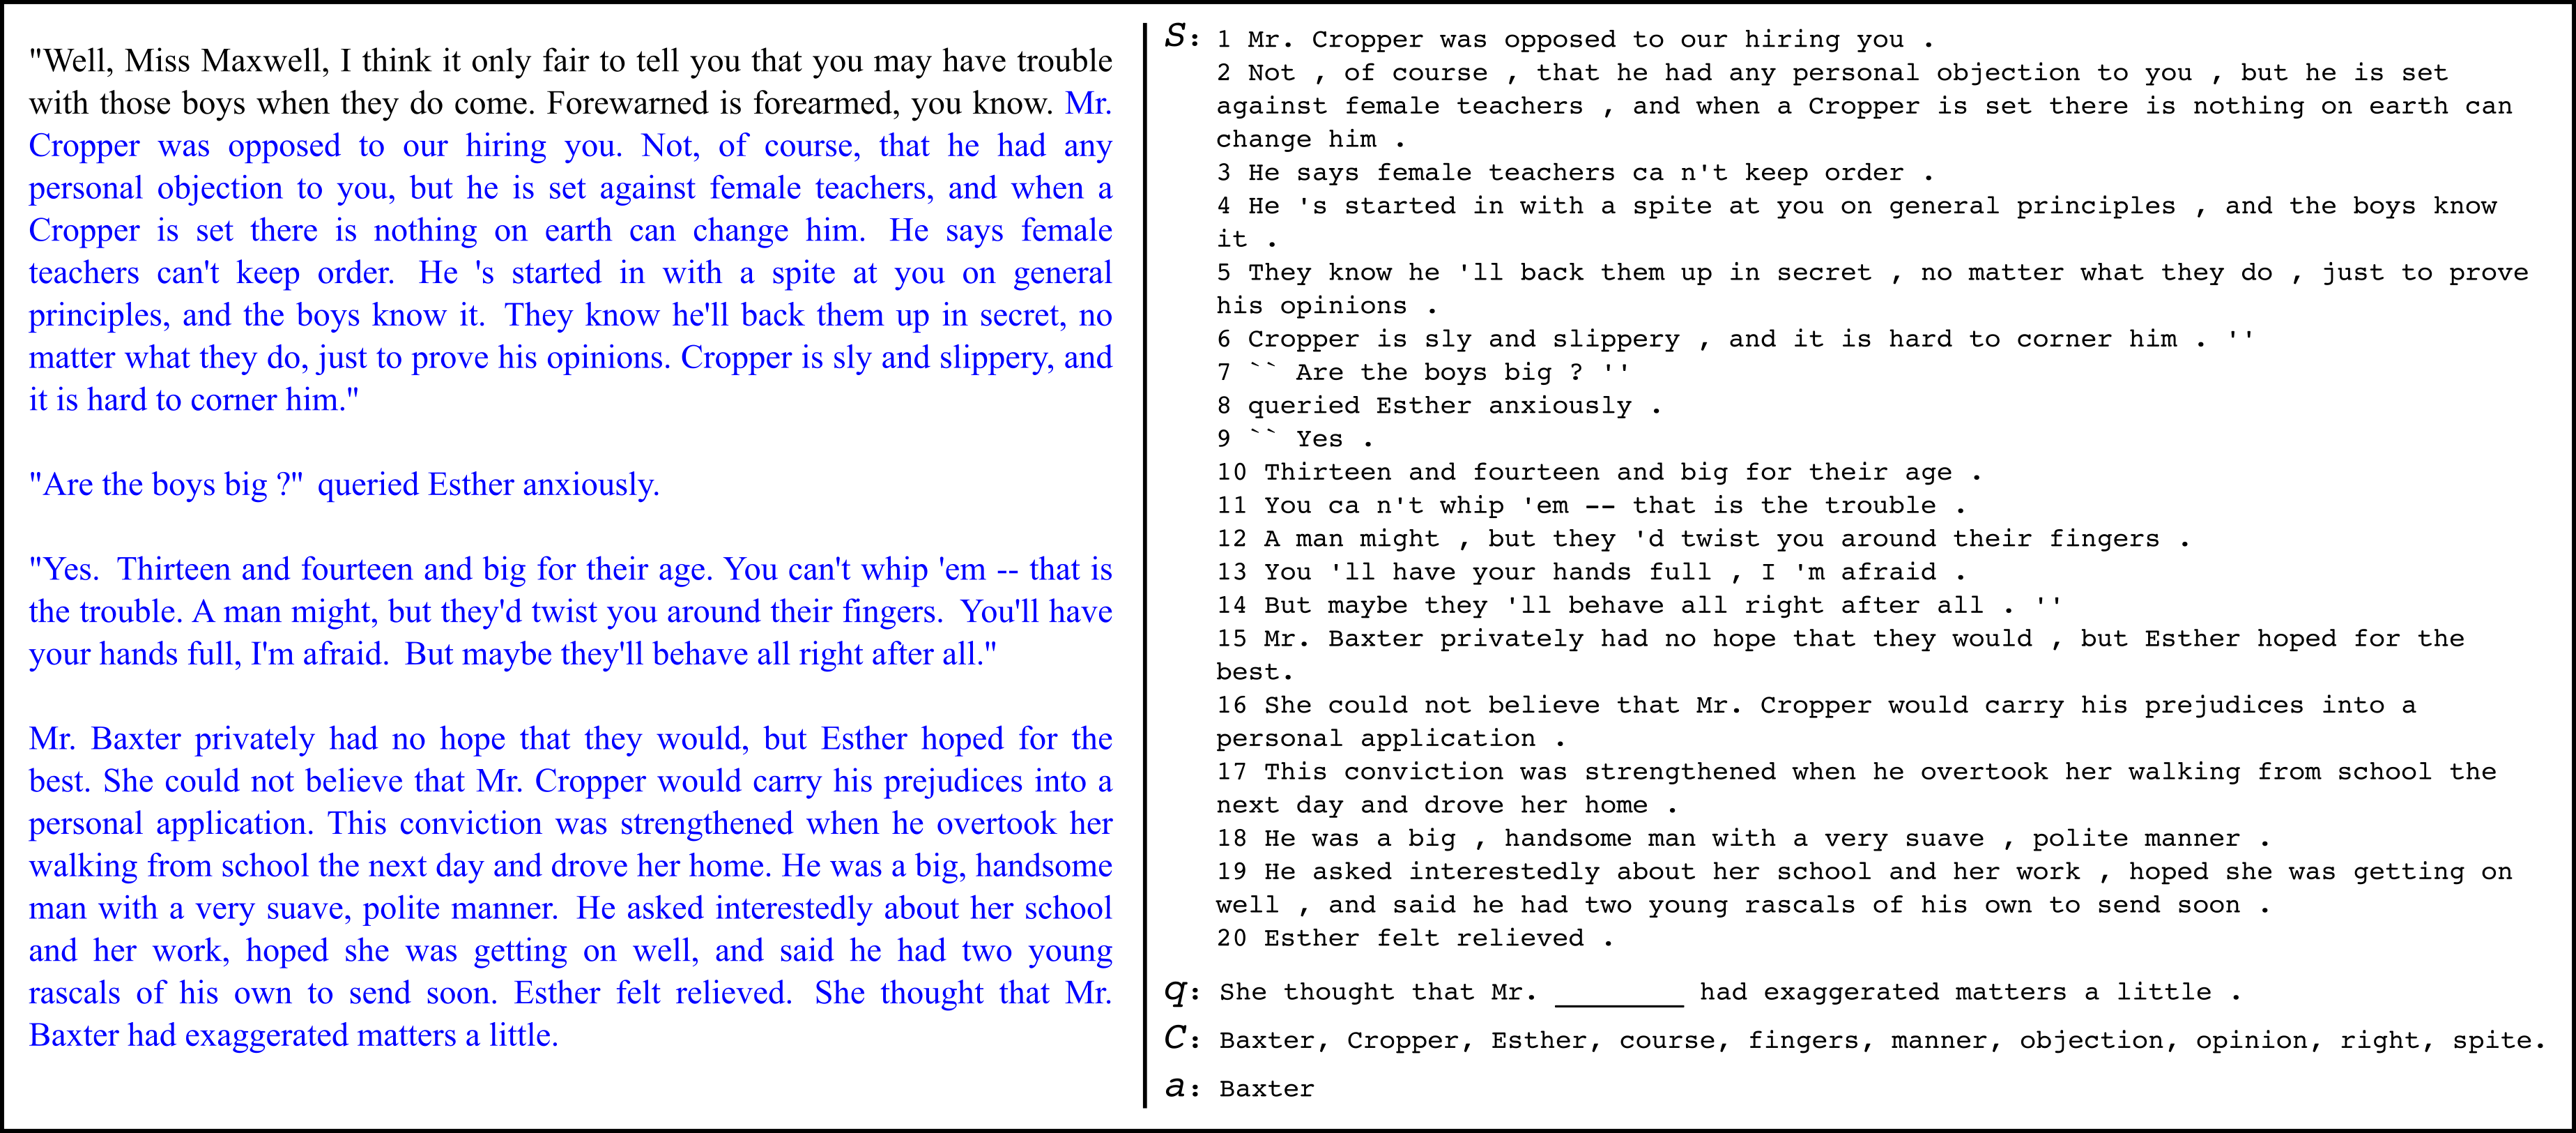
\includegraphics[width=\textwidth]{Chapter_6/cbt_fig1.png}
\caption{{\bf A Named Entity question from the CBT} (right), created from a book passage (left, in blue). In this case, the candidate answers \(C\) are both entities and common nouns, since fewer than ten named entities are found in the context.}
\label{fig:goldilocks}
\end{figure}

For finer-grained analyses, I created four classes of question by removing distinct types of word: Named Entities, (Common) Nouns, Verbs and Prepositions (based on output from the POS tagger and named-entity-recogniser in the Stanford Core NLP Toolkit \citep{manning2014stanford}). For a given question class, the nine incorrect candidates are selected at random from words in the context having the same type as the answer. The exact number of questions in the training, validation and test sets is shown in Table \ref{tab:cbt_stat}. Full details of the candidate selection algorithm (e.g. how candidates are selected if there are insufficient words of a given type in the context) can be found with the dataset.\footnote{The dataset can be downloaded from \url{http://fb.ai/babi/}.}

Classical language modelling evaluations are based on average perplexity across all words in a text. They therefore place proportionally more emphasis on accurate prediction of frequent words such as prepositions and articles than the less frequent words that transmit the bulk of the meaning in language \citep{baayen1996word}. In contrast, because the CBT allows focused analyses on semantic content-bearing words, it should be a better proxy for how well a language model can lend semantic coherence to applications including machine translation, dialogue and question-answering systems. 


\vspace{-2mm}
\begin{table}[ht]
\label{tab:cbt_stat}
  \begin{center}
    {\small 
      {\sc 
        \begin{tabular}{l|ccc}
          & Training & Validation & Test \\
          \hline
          \hline
          Number of books & 98 & 5 & 5 \\
          Number of questions (context+query)& 669,343 & 8,000 & 10,000  \\
          Average words in contexts & 465 & 435 & 445 \\
          Average words in queries & 31 & 27 & 29 \\
          Distinct candidates & 37,242 & 5,485 & 7,108 \\
          \hline
          Vocabulary size & \multicolumn{3}{|c}{53,628}\\
          \hline
        \end{tabular}
      }
    }
    \caption{\label{tab:cbt_stat} {\bf Statistics of the CBT.} Breakdown by question class is provided with the data set files.}
  \end{center}
\vspace*{-4ex}
\end{table}



%\begin{listenv}{An example question from the Named Entities section of the CBTest dataset, taken from The Jungle Book.} \itemsep1pt \parskip0pt \parsep0pt
%\tiny{
 % \item[C1] I will play with them again . ''
  %\item[C2]  `` Listen , man-cub , '' said the Bear , and his voice rumbled like thunder on a hot night .
  %\item[C3]   `` I have taught thee all the Law of the Jungle for all the peoples of the jungle -- except the Monkey-Folk who live in the trees .	
  %\item[C4]   They have no law .
  %\item[C5]   They are outcasts .
  %\item[C6]   They have no speech of their own , but use the stolen words which they overhear when they listen , and peep , and wait up above in the branches .
  %\item[C7]   Their way is not the way .
  %\item[C8]   They are without leaders .
  %\item[C9]   They have no remembrance .
  %\item[C10]   They boast and chatter and pretend that they are a great people about to do great affairs in the jungle , but the falling of a nut turns their minds to laughter and all is forgotten .
  %\item[C11]   I of the jungle have no dealings with them .
  %\item[C12]   I do not drink where the monkeys drink ; I do not go where the monkeys go ; I do not hunt where they hunt ; I do not die where they die .
  %\item[C13]   Hast thou ever heard me speak of the Bandar-log till today ? ''
  %\item[C14]   `` No , '' said Mowgli in a whisper , for the forest was very still now Baloo had finished .
  %\item[C15]   `` The Jungle-People put them out of their mouths and out of their minds .
  %\item[C16]   They are very many , evil , dirty , shameless , and they desire , if they have any fixed desire , to be noticed by the Jungle People .
  %\item[C17]   But I do not notice them even when they throw nuts and filth on the heads . ''
  %\item[C18]   He had hardly spoken when a shower of nuts and twigs spattered down through the branches ; and they could hear coughings and howlings and angry jumpings high up in the air among the thin branches.
  %\item[C19]   `` The Monkey-People are forbidden , '' said Baloo , `` forbidden to the Jungle-People ."
  %\item[C20]   Remember . 
  %\item[Query]   `` Forbidden , '' said Bagheera , `` but I still think \   \textunderscore\textunderscore\textunderscore\textunderscore\textunderscore\textunderscore \  should have warned thee against them ." 
  %\item[Answer]   Baloo 
  %\item[Candidates]    Bear|Bandar-log|Baloo|Jungle-People|Monkey-People|Mowgli|coughings|howlings|jumpings|man-cub
%}
%\end{listenv}
 

%\end{nonfloatlistenv}

\subsection{Related resources}
There are clear parallels between the CBT and the Microsoft Research Sentence Completion Challenge (MSRCC) \citep{zweig2011microsoft}, which is also based on Project Gutenberg (but not children's books, specifically). A fundamental difference is that, where examples in the MSRCC are made of a single sentence, each query in the CBT comes with a wider context. This tests the sensitivity of language models to semantic coherence beyond sentence boundaries. The CBT is also larger than the MRSCC (10,000 vs 1,040 test questions), requires models to select from more candidates on each question (10 vs 5), covers missing words of different (POS) types and contains large training and validation sets that match the form of the test set. 

There are also similarities between the CBT and the CNN/Daily Mail (CNN QA) dataset recently released by \cite{nips15_hermann}. This task requires models to identify missing entities from bullet-point summaries of online news articles. The CNN QA task therefore focuses more on paraphrasing parts of a text, rather than making inferences and predictions from contexts as in the CBT. It also differs in that all named entities in both questions and articles are anonymised so that models cannot apply knowledge that is not apparent from the article. I do not anonymise entities in the CBT, as I hope to incentivise models that can apply background knowledge and information from immediate and wider contexts to the language understanding problem.\footnote{See Appendix~\ref{ap:anon} for a sense of how anonymisation changes the CBT.} At the same time, the CBT can be used as a benchmark for general-purpose language models whose downstream application is semantically focused generation, prediction or correction. 
%
The CBT is also similar to the MCTest of machine comprehension \citep{richardson2013mctest}, in which children's stories written by annotators are accompanied by four multiple-choice questions. However, it is very difficult to train statistical models only on MCTest because its training set consists of only 300 examples.

\section{Memory representation in memory networks}

\label{sec:memnn}

Context sentences of $S$ are encoded into memories, denoted $m_i$, using a feature-map \(\phi(s)\) mapping sequences of words \(s \in S\) from the context to one-hot representations in \([0,1]^d\), where $d$ is typically the size of the word vocabulary. Memory networks are a comparatively new technology, and can be challenging to train as each constituent component must be optimised via a single error signal backpropagated from the output predictions. Indeed, this work constitutes their first application to naturally occurring language. We therefore constrain our analyses to three simple (word-order independent) forms for forming representations \(s\) of the context, detailed below. Ultimately, however, as the infrastructure challenges reduce, the prior structures and representational forms for word, phrase or sentence representation treated in Chapters~\ref{CH2}-\ref{CH5} could also be used and might lead to improved results.

\begin{itemize}  %  [leftmargin=3mm]

\item {\bf Lexical memory:} Each word occupies a separate slot in the memory (each phrase \(s\) is a single word and \(\phi(s)\) has only one non-zero feature). To encode word order, time features are added as embeddings indicating the index of each memory, following \cite{sukhbaatar2015end}. 

\item {\bf Window memory:} Each phrase \(s\) corresponds to a window of text from the context $S$ centred on an individual mention of a candidate $c$ in $S$. Hence, memory slots are filled using windows of words \(\{ w_{i-(b-1)/2} \dots w_i \dots w_{i+(b-1)/2} \} \) where \(w_i\in C\) is an instance of one of the candidate words in the question.\footnote{See Appendix~\ref{ap:nonsparse-windows} for discussion and analysis of using candidates in window representations and training.} Note that the number of phrases \(s\) is typically greater than $|C|$ since candidates can occur multiple times in $S$. The window size \(b\) is tuned on the validation set. I experimented with encoding as a standard bag-of-words, or by having one dictionary per window position, where the latter performed best.

\item {\bf Sentential memory:} This setting follows the original implementation of Memory Networks for the bAbI tasks where the phrases \(s\) correspond to complete sentences of $S$.  For the CBT, this means that each question yields exactly 20 memories. I also experiment with or without Positional Encoding (PE) as introduced by \cite{sukhbaatar2015end} to encode the word positions. 
\end{itemize}

The order of occurrence of memories is less important for sentential and window formats than for lexical memory. So, instead of using a full embedding for each time index, I simply use a scalar value which indicates the position in the passage, ranging from 1 to the number of memories. An additional parameter (tuned on the validation set) scales the importance of this feature. As I show in Appendix~\ref{ap:qa_cnn_ab_study}, time features only gave a marginal performance boost in those cases.

% In \citep{weston2014memory} the idea of attaching time features to memories is proposed so that the model is aware of which memories ``occur'' first, which was shown vital in some synthetic natural language tasks. Here, I implemented a very simple variant: each memory has an additional scalar feature ${\mbox{t}}(m')$ which indicates its position in the passage, ranging from 1 to the memory size. Scoring of a memory then becomes:
% \[
%    S_{time}(q, m') =  S(q, y) + \beta~ {\mbox{time}}(m')
% \]
% where an additional parameter $\beta$ (tuned on the validation set) indicates the importance of the time feature. However, as I will see in the experiments, this only gave a marginal performance boost on the tasks I consider in this paper.
% Note that, because time features are encoded in the memory (see below), this effectively models the memory as an ordered stream of individual words.  

For sentential and window memory formats, queries are encoded in a similar way to the memories: as a bag-of-words representation of the whole sentence and a window of size $b$ centred around the missing word position respectively.
%
For the lexical memory, memories are made of the $n$ words preceding the word to be predicted, whether these $n$ words come from the context or from the query, and the query embedding is set to a constant vector $0.1$. 

\subsection{End-to-end training} \label{sec:mod_o}

The {MemN2N} architecture, introduced by \cite{sukhbaatar2015end}, allows for direct training of memory networks with backpropagation.

First, `supporting memories', those useful to find the correct answer to the query $q$, are retrieved. This is done by embedding both the query and all memories into a single space of dimension $p$ using an embedding matrix $\bA\in\Re^{p \times d}$ yielding the query embedding  $\bq=\bA\phi(q)$ and memory embeddings $\{\bc_i=\bA\phi(s_i)\}_{i=1,\dots n}$, with $n$ the number of memories. %\footnote{To encode the position of words in the windows on the window memory setting, I used one embedding matrix per position, that is, $\bA$ is duplicated $b$ times.} 
%
\if0 %old stuff
The match between $\bq$ and each memory $\bc_i$ in the embedding space is fed through a softmax layer giving a distribution \(\{\alpha_i\}_{i=1, \dots n}\) of matching scores defined by $\alpha_i =  e^{\bc_i^\top\bq} / \sum_j e^{\bc_j^\top\bq}$. These weights are used to return a weighted average of memories as the first supporting memory:\footnote{Such a weighted average over memories can also be understood as the model's \emph{attention} mechanism.} 
\begin{equation} \label{eq:eq_o}
  \bm_{o1} = \sum_{i=1 \dots n} \alpha_{i} \bm_i \,,
\end{equation}
\fi
The match between $\bq$ and each memory $\bc_i$ in the embedding space is fed through a softmax layer giving a distribution \(\{\alpha_i\}_{i=1, \dots n}\) of matching scores which are used as an \emph{attention} mechanism over the memories to return the first supporting memory:%\footnote{Such a weighted average over memories can also be understood as.} 
\begin{equation} \label{eq:eq_o}
  \bm_{o1} = \sum_{i=1 \dots n} \alpha_{i} \bm_i\,, \mbox{~~~~~~}\text{with~~~~~}\alpha_i =  \frac{e^{\bc_i^\top\bq}}{\sum_j e^{\bc_j^\top\bq}}, \, i=1,\dots n,
\end{equation}
and where $\{\bm_i\}_{i=1,\dots n}$ is a set of memory embeddings obtained in the same way as the $\bc_i$, but using another embedding matrix $\bB\in\Re^{p\times d}$. During training, optimization is carried out using stochastic gradient descent (SGD). Extra experimental details and hyperparameters are given in Appendix~\ref{ap:hp}.

%\todo{something about multi-core training: AB: not sure especially since word-memnn run on GPU. seems to complexify for nothing.}. 


\subsection{Self-supervision for Window Memories} \label{sec:ssup}

%The softmax operation over memories in eq~\eqref{eq:eq_o} of the ${\bf O}$ module can dilute information across the whole context in cases where a single memory is enough to answer correctly. 

Training a memory network with multiple components by backpropagating a single error signal derived from its final predictions can constitute a challenging non-convex optimisation problem. After initial experiments, I found that it was beneficial to use a heuristic to provide a stronger signal for learning memory access. A related approach was successfully applied by \cite{bordes2015large} to question answering about knowledge bases.

\if0
In a `self-supervised' Memory Network, a heuristic informs the network which memories to attend to for each training question. Intuitively, this can help to overcome the difficult optimization inherent in training a single network jointly to access information and use it effectively. For the CBT, the heuristic identifies potentially correct memories as those whose corresponding candidate is the correct answer. In the common case where more than one memory contains the correct answer, the heuristic picks the single memory $\tilde{m}$ that is scored highest by the query in the embedding space defined by $\bA$.\footnote{TF-IDF similarity worked almost as well in the experiments, but a random choice over positives did not.} The model incorporates this information by taking a gradient step using SGD to force its memory retrieval network, for each example, to give a higher score to the supporting memory $\tilde{m}$ than other memories.
\fi

		
Memory supervision (knowing which memories to attend to) is not provided at training time but is inferred automatically using a simple heuristic: during training, the correct supporting memory is assumed to be among the window memories whose corresponding candidate is the correct answer.		
%		
In the common case where more than one memory contains the correct answer, the model picks the single memory $\tilde{m}$ that is already scored highest by itself, i.e. scored highest by the query in the embedding space defined by $\bA$.\footnote{TF-IDF similarity worked almost as well in the experiments, but a random choice over positives did not.} 

Training is carried out by making gradient steps using SGD to force the model, for each example, to give a higher score to the supporting memory $\tilde{m}$ relative to any other memory from any other candidate.
%
Instead of using  eq~\eqref{eq:eq_o}, the model selects its top relevant memory using:
\begin{equation} \label{eq:salient}
  m_{o1} = \argmax_{i=1,\dots n} \bc_i^\top\bq \, .%\footnote{This hard selection was actually used in the original Memory Network paper \citep{weston2014memory}}
\end{equation}
%
If $m_{o1}$ happens to be different from $\tilde{m}$, then the model is updated.


%

%


%
At test time, rather than use a hard selection as in eq~\eqref{eq:salient}
the model scores each candidate not only with its highest scoring memory
but with the sum of the scores of all its corresponding windows after passing all scores through a softmax. That is, the score of a candidate is defined by the sum of the $\alpha_i$ (as used in eq~\eqref{eq:eq_o}) of the windows it appears in. This relaxes the effects of the \(max\) operation and allows for all windows associated with a candidate to contribute some information about that candidate. As shown in the ablation study in Appendix~\ref{ap:qa_cnn_ab_study}, this results in slightly better performance on the CNN QA benchmark compared to hard selection at test time.

Note that self-supervised Memory Networks do not exploit any new label information beyond the training data. % (compared to e.g. the strong supervision in the bAbI tasks of \cite{}).
The approach can be understood as a way of achieving \emph{hard attention} over memories, to contrast with the \emph{soft attention}-style selection described in Section~\ref{sec:mod_o}. Hard attention yields significant improvements in image captioning \citep{xu2015show}. However, where \cite{xu2015show} use the REINFORCE algorithm \citep{williams1992simple} to train through the max of eq~\eqref{eq:salient}, the self-supervision heuristic permits direct backpropagation.


% In the common case where more than one memory contains the correct answer, I select the favored memory using one of two strategies:
% \begin{itemize}
% \item[(i)] Select the memory containing the correct answer that also has the with highest TFDIF bag-of-words score with the query as the supervised target.
% \item[(ii)] Use the model itself selects the highest scoring of all memories that contain the correct answer. 
% \end{itemize}
% Both approaches end up working quite well in the experiments. 

%\todo{I am a little concerned this paragraph seems to contradict the first paragraph in this section   "The softmax operation....". What do you think?}


% One can thus instead consider the scoring function:
% \[
% a = \argmax_{w \in W}\{ S_R(q,w) + S_R(\textbf{m}_1,w)
%   + \alpha \sum_{k : y(m_k) = y(m_1)} S_R(\textbf{m}_k,w)  \}
% \]
% where $y(m')$ is the label (output candidate word) for the memory $m'$. Note that this approach is only viable for the window memory approach where each memory is associated with an explicit candidate. This gives one more parameter, $\alpha$, to be learnt.

\section{Baseline and ocmparison models}


In addition to memory network variants, I also applied many different types of
 language modelling and machine reading architectures to the CBT.
%To place the performance of different Memory Network designs in context, I also applied 
%various existing language modelling and machine reading architectures to the CBT.

\subsection{Non-learning baselines}
I implemented two simple baselines based on word frequencies. For the first, I selected the most frequent candidate in the entire training corpus. In the second, for a given question I selected the most frequent candidate in its context. In both cases I broke ties with a random choice. 

I also tried two more sophisticated ways to rank the candidates that do not require any learning on the training data. The first is the `sliding window' baseline applied to the MCTest by \cite{richardson2013mctest}. In this method, ten `windows' of the query concatenated with each possible candidate are slid across the context word-by-word, overlapping with a different subsequence at each position. The overlap score at a given position is simply word-overlap weighted TFIDF-style based on frequencies in the context (to emphasize less frequent words). The chosen candidate corresponds to the window that achieves the maximum single overlap score for any position. Ties are broken randomly. 

The second method is the word distance benchmark applied by \cite{nips15_hermann}. For a given instance of a candidate \(w_i\) in the context, the query \(q\) is `superimposed' on the context so that the missing word lines up with \(w_i\), defining a subsequence \(s\) of the context. For each word \(q_i\) in \(q\), an alignment penalty $P = \min( \min_{j = 1 \dots |s|} \{|i - j| : s_j = q_i\}, m)$ is incurred. The model predicts the candidate with the instance in the context that incurs the lowest alignment penalty. I tuned the maximum single penalty \(m=5\)  on the validation data.  

\subsection{N-gram language models}
I trained an n-gram language model using the KenLM toolkit \citep{Heafield-estimate}. I used Knesser-Ney smoothing, and a window size of 5, which performed best on the validation set.
%
I also compare with a variant of language model with cache \citep{kuhn1990cache}, where I linearly interpolate the n-gram model probabilities with unigram probabilities computed on the context.

\subsection{Supervised embedding models}
To directly test how much of the CBT can be resolved by good quality dense representations of words (word embeddings), I implement a supervised embedding model similar to that of \citep{weston2010large}. In these models I learn both input and output embedding matrices \(\bA,\,\bB \in \Re^{p\times d}\) for each word in the vocabulary ($p$ is still the embedding dimension and $d$ the vocabulary size). For a given input passage \(q\) and possible answer word \(w\), the score is computed as \(S(q,\,w) = \phi(q) \bA ^\top \bB \phi(w) \), with \(\phi\) the feature function defined in Section~\ref{sec:memnn}.
These models can be considered as lobotomised Memory Networks with zero hops, 
i.e. the attention over the memory component is removed.

I encode various parts of the question as the input passage: the entire {\bf context + query}, just the {\bf query}, a sub-sequence of the query defined by a {\bf window} of maximum \(b\) words centred around the missing word, and a version ({\bf window + position}) in which I use a different embedding matrix  for encoding each position of the window. I tune the window-size \(d=5\) on the validation set. 


\subsection{Recurrent language models}
I trained probabilistic RNN language models with LSTM activation units on the training stories (5.5M words of text) using minibatch SGD to maximise the negative log-likelihood of the next word. Hyper-parameters were tuned on the validation set. The best model had both hidden layer and word embeddings of dimension $512$.
%
When answering the questions in the CBT, I allow one variant of this model ({\bf context + query}) to `burn in' by reading the entire context followed by the query and another version to read only the {\bf query} itself (and thus have no access to the context). Unlike the canonical language-modelling task, all models have access to the query words {\em after} the missing word (i.e if $k$ is the position of the missing word, I rank candidate \(c\) based on \(p(q_1 \dots q_{k-1}, c , q_{k+1} \dots q_l)\) rather than simply \(p(q_1 \dots q_{k-1},c)\)).

\cite{mikolov2012context} previously observed performance boosts for recurrent language models by adding the capacity to jointly learn a document-level representation. I similarly apply a context-based recurrent model to the language-modelling tasks, but opt for the convolutional representation of the context applied by \cite{rush2015neural} for summarisation. the Contextual LSTM (CLSTM) learns a convolutional attention over windows of the context given the objective of predicting all words in the query. I tuned the window size (\(w=5\)) on the validation set. As with the standard LSTM, I trained the CLSTM on the running-text of the CBT training set (rather than the structured query and context format used with the Memory Networks) since this proved much more effective, and I  report results in the best setting for each method.

\subsection{Human performance}

I recruited 15 native English speakers to attempt a randomly-selected 10\% from each question type of the CBT, in two modes either with question only or with question+context (shown to different annotators), giving 2000 answers in total.
 % so that each annotator answered $\approx$ 132 questions. 
To the knowledge, this is the first time human performance has been quantified on a language modelling task based on %multiple participants and 
different word types and context lengths.

%As a result, I do not have a measure of the variance of the human judgements but I have a better coverage of questions, which was the priority.

\subsection{Other related approaches}
The idea of conditioning language models on extra-sentential context is not new. Access to document-level features can improve both classical language models \citep{mikolov2012context} and word embeddings \citep{huang2012improving}. Unlike the present work, these studies did not explore different representation strategies for the wider context or their effect on interpreting and predicting specific word types.

The original Memory Networks \citep{weston2014memory} used hard memory selection with additional labeled supervision for the memory access component, and
%used self-supervised memory access and were 
were applied to question-answering tasks 
%in which language was generated to describe the content of 
over knowledge bases or simulated worlds. \cite{sukhbaatar2015end} and \cite{kumar2015ask} trained Memory Networks with RNN components end-to-end with soft memory access, and applied them to additional language tasks. The attention-based reading models of \cite{nips15_hermann} also have many commonalities with Memory Networks, differing in word representation choices 
and attention procedures.
%I guess I don't want to emphasize this so much if it doesnt work: %, one key difference being the absence of iterative access, based on the entire query, to the memory-like representations.
Both \cite{kumar2015ask} and \cite{nips15_hermann} propose bidirectional RNNs as a way of representing previously read text. the experiments in Section~\ref{sec:results} provide a possible explanation for why this is an effective strategy for semantically-focused language processing: bidirectional RNNs naturally focus on small windows of text in similar way to window-based Memory Networks. 

Other recent papers have proposed RNN-like architectures with new ways of reading, storing and updating information to improve their capacity to learn algorithmic or syntactic patterns \citep{joulin2015inferring,dyer2015transition,grefenstette2015learning}. While I do not study these models in the present work, the CBT would be ideally suited for testing this class of model on semantically-focused language modelling.  

\section{Results}


\label{sec:results}

\begin{table}[t]
\newcommand{\mc}[1]{\multicolumn{1}{l|}{#1}}
  \begin{center}
    \resizebox{1\linewidth}{!}{
      {\sc 
        \begin{tabular}{l|cccc}
          \mc{Methods} & Named Entities & Common Nouns & Verbs & Prepositions
          \\
          \hline
          \hline
          \mc{Humans (query)$^{(*)}$} & 0.520 & 0.644 & 0.716 & 0.676 \\
          \mc{Humans (context+query)$^{(*)}$} &{\it \textbf{0.816}} & {\it \textbf{ 0.816}} & {\it \textbf{0.828}} & 0.708 \\
          \hline 
          \hline 
          \mc{Maximum frequency (corpus)} & 0.120 & 0.158 & 0.373 & 0.315 \\
          \mc{Maximum frequency (context)} & 0.335 & 0.281 & 0.285 & 0.275 \\
          \mc{Sliding window} & 0.168 & 0.196 & 0.182 & 0.101 \\
          \mc{Word distance model} & 0.398 & 0.364 & 0.380 & 0.237 \\
          \mc{Kneser-Ney language model} & 0.390 & 0.544 & 0.778 & 0.768 \\                                                                    
          \mc{Kneser-Ney language model + cache} & 0.439 & 0.577 & 0.772 & 0.679 \\ 
          \hline
          \mc{\starspace (context+query)} & 0.253 & 0.259 & 0.421 & 0.315 \\
          \mc{\starspace (query)} & 0.351 & 0.400 & 0.614 & 0.535 \\
          \mc{\starspace (window)} & 0.362 & 0.415 & 0.637 & 0.589 \\
          \mc{\starspace (window+position)} & 0.402 & 0.506 & 0.736 & 0.670 \\
          \hline 
          \mc{LSTMs (query)} & 0.408 & 0.541 & 0.813 & 0.802 \\
          \mc{LSTMs (context+query)} & 0.418 & 0.560 & \bf 0.818 & 0.791 \\
          \mc{Contextual LSTMs (window context)} & 0.436 & 0.582 & 0.805 & \bf 0.806\\
          \hline
          \hline
          MemNNs  (lexical memory) &   0.431 & 0.562 & 0.798 & 0.764 \\
          MemNNs  (window memory) &  0.493 & 0.554 & 0.692 & 0.674 \\
          MemNNs  (sentential memory + PE) & 0.318 & 0.305 & 0.502 & 0.326 \\
          MemNNs  (window memory + self-sup.) & \bf 0.666 & \bf 0.630 & 0.690 & 0.703\\
          \hline 
          %MemNNs  (window + self-sup. + anonym.) & 0.581 & 0.473 & 0.474 & 0.522\\
          %\hline
        \end{tabular}
      }
    }
    \caption{\label{tab:cbt_res} {\bf Results on CBT test set.} $^{(*)}$Human results were
      collected on 10\% of the test set.}\label{tab:cbt_res}
  \end{center}
  \vspace*{-4ex}
\end{table}

\paragraph{The form of memory representations} Of central importance to this thesis is the fact that the particular form of the internal memory representations had a clear impact of the performance of memory networks.

 When each sentence in the context is stored as an ordered sequence of word embeddings (\emph{sentence mem + PE}), performance is generally poor. Encoding the context as an unbroken sequence of individual words (\emph{lexical memory}) works particularly well for capturing prepositions and verbs, but is less effective with nouns and entities. In contrast, \emph{window memories} centred around the candidate words are more useful than either word-level or sentence-level memories when predicting named entities and nouns. 


It is tempting to ascribe the poor performance of full-sentence embeddings to the limitations of bag-of-words encoding (and the blindness to word order). However, for nouns and named entity prediction, networks with memories that do not encode word order (window memories) ara capable of outperforming those that do (both lexical memories and the DeepMind bidirectional RNN reading models~\citep{nips15_hermann} discussed in Section~\ref{dmind}). This suggests that word order itself is of secondary importance compared with the `scope' of the representation. In particular, it appears that full sentences in general contain too much disparate information for the pertinent parts to be easily accessed if encoded into a single representation. 

Of course, it is important to note that these conclusions relat only to the present (word-prediction) task and the CNN QA task described below. The extent to which they generalise remains to be determined by future work. 

\paragraph{Modelling syntactic flow} 
In general, there is a clear difference in model performance according
to the type of word to be predicted. the main results in Table \ref{tab:cbt_res}
%As can be seen in Table
%\ref{tab:cbt_res}, conventional language models are very good at
show  conventional language models are very good at
predicting prepositions and verbs, but less good at predicting named
entities and nouns. Among these language models, and in keeping with
established results, RNNs with LSTMs demonstrate a small gain on
n-gram models across the board, except for named entities where the cache is beneficial. 
In fact, LSTM models are better than humans at predicting prepositions, which suggests that there are cases in which several of the candidate prepositions are `correct', but annotators prefer the less frequent one.  Even more surprisingly, when only local context (the query) is available, both LSTMs and n-gram models predict verbs more accurately than humans. This may be because the models are better attuned to the distribution of verbs in children's books, whereas humans are unhelpfully influenced by their wider knowledge of all language styles.\footnote{I did not require the human annotators warm up by reading the 98 novels in the training data, but this might have led to a fairer comparison.} When access to the full context is available, humans do predict verbs with slightly greater accuracy than RNNs. 

\paragraph{Capturing semantic coherence} The best performing Memory
Networks predict common nouns and named entities more
accurately than conventional language models. Clearly, in doing so,
these models rely on access to the wider context (the
supervised {\small \sc{embedding model (query)}}, which is equivalent to the
memory network but with no contextual memory, performs poorly in this
regard). The fact that LSTMs without attention perform similarly on
nouns and named entities whether or not the context is available
confirms that they do not effectively exploit this context. This may
be a symptom of the difficulty of storing and retaining information
across large numbers of time steps that has been previously observed
in recurrent networks (See e.g. \cite{bengio1994learning}). 
%LSTMs have been shown to do well
%on tasks such as 
%translation between close languages \cite{sutskever2014sequence} but note that only consists of a single source sentence.

%LSTMs are able to overcome this issue for related problems such as translation between close languages \cite{sutskever2014sequence}. The reason that they cannot in the present case may be due to the low frequency of nouns and entities and the nature of the missing word prediction task, which together make it challenging for the multiple memory gates to learn information retention strategies that effectively generalise to the test set. 



%
%This is confirmed by the strong performance of the CLSTM implementation,
%which also relies on attention over window-like representations of the context.
% indicate the great fit of
%this format for this task.

\begin{figure}[ht]
\newcommand{\mc}[1]{\multicolumn{2}{l}{#1}}
  \begin{center}
   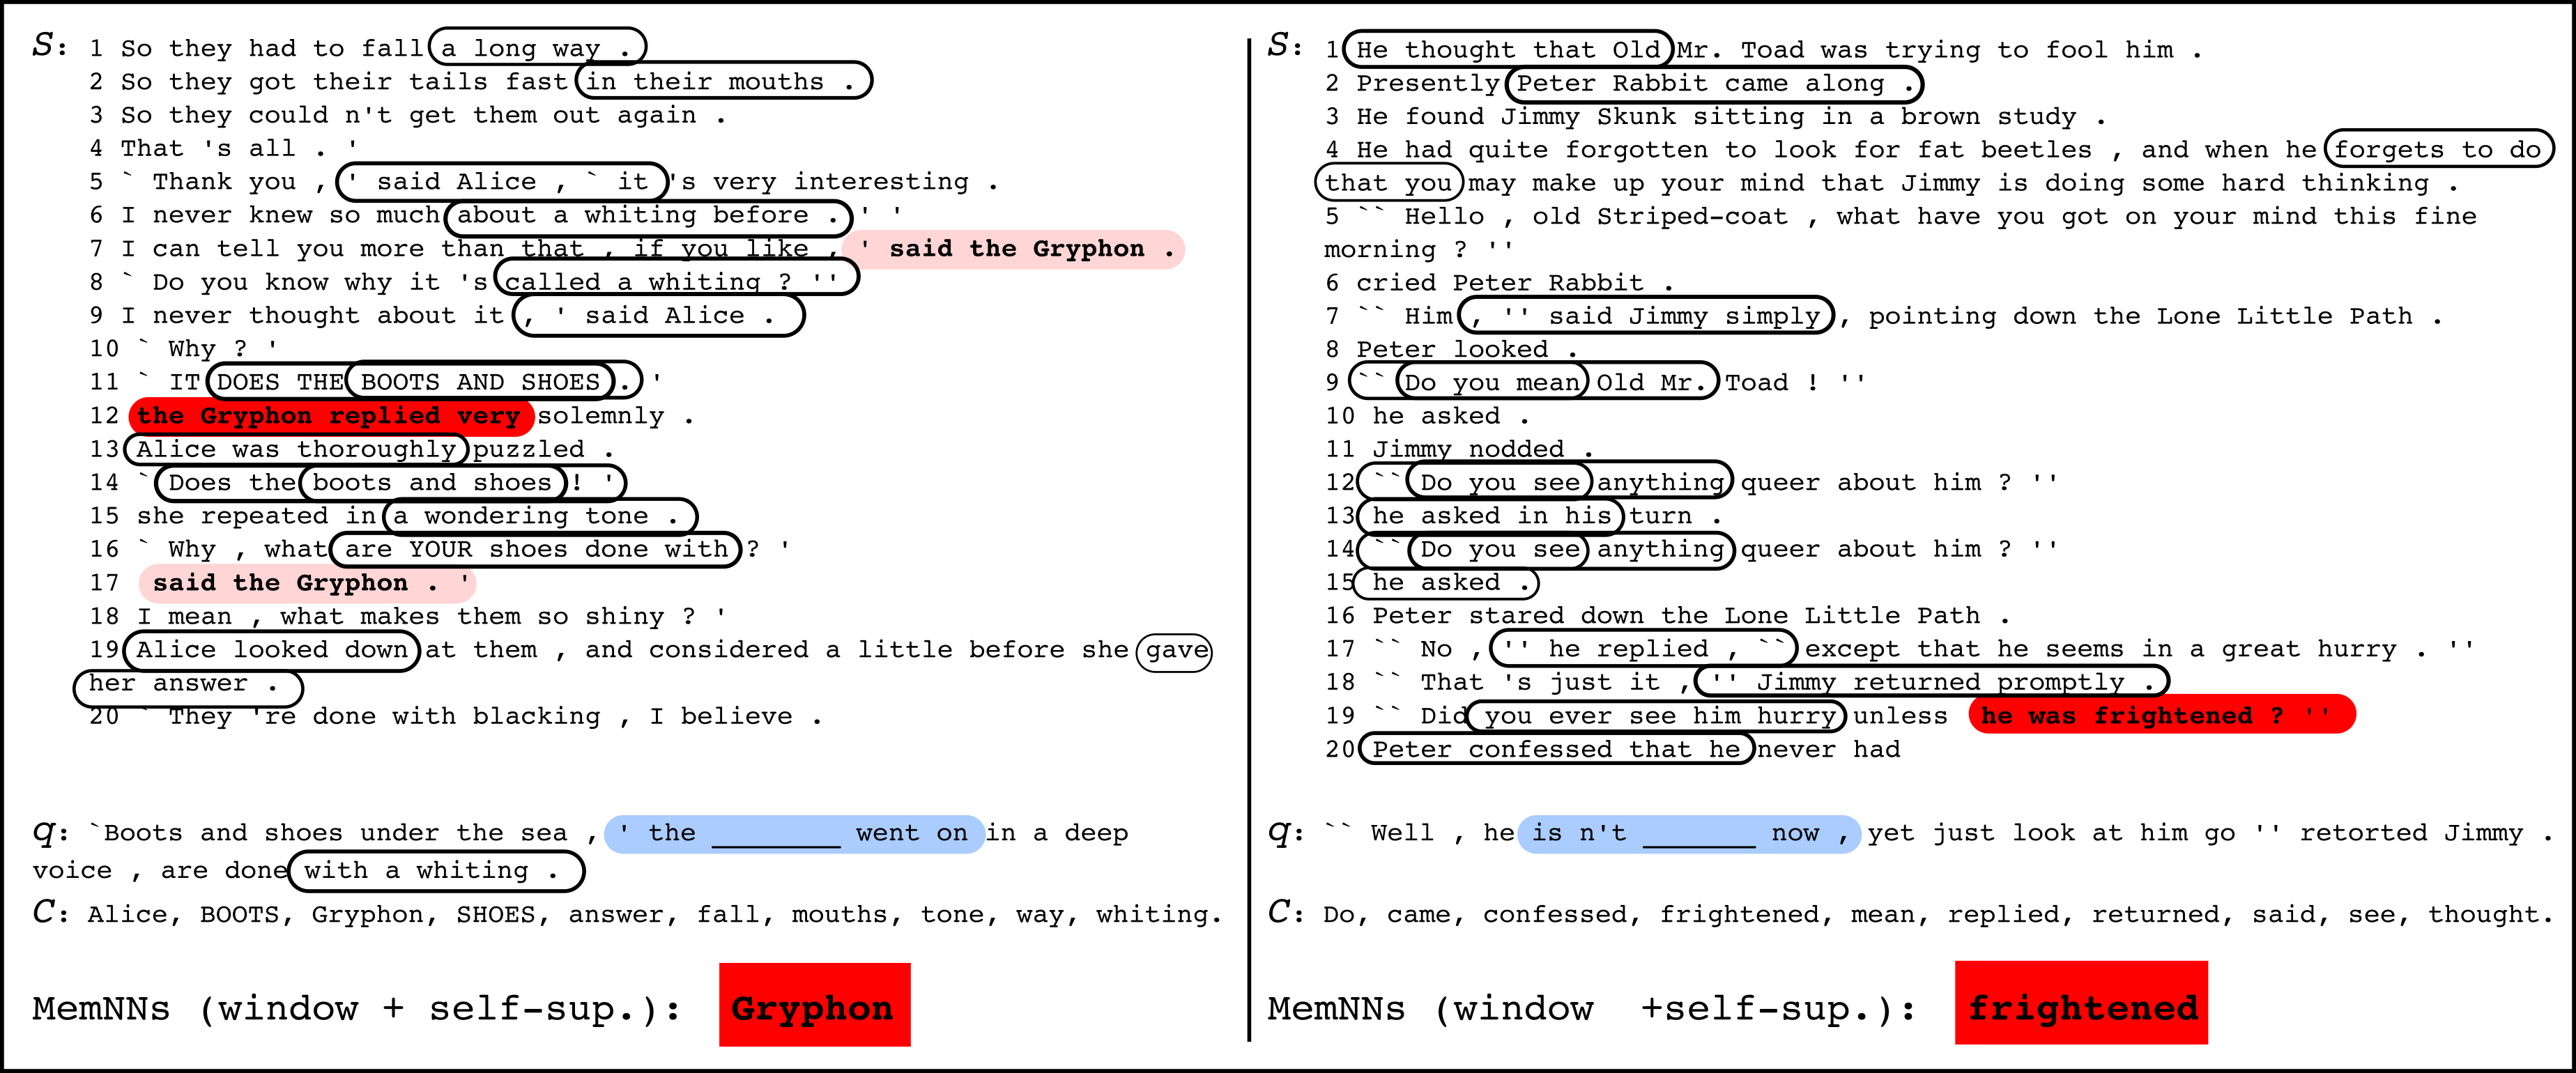
\includegraphics[width=\textwidth]{Chapter_6/cbt_fig2.png}
      \caption{\label{tab:ex_pred_cbt} {\bf Correct predictions of
          MemNNs (window memory + self-supervision) on CBT} on Named Entity (left) and
          Verb (right). Circled phrases indicate all considered
          windows; red ones are the ones corresponding to the returned
          (correct) answer; the blue windows represent the queries.}\label{tab:ex_pred_cbt}
    \end{center}
  \vspace*{-2ex}
\end{figure}


\paragraph{Self-supervised memory retrieval} 
%
The window-based Memory Network with self-supervision (in which a hard attention selection 
is made among window memories during training)
outperforms all others at predicting named entities and common nouns.
%
%Examples of predictions of this model for two CBT questions are shown in Figure~\ref{tab:ex_pred_cbt}. 
%
Examples of predictions made by this model for two CBT questions are shown
in Figure~\ref{tab:ex_pred_cbt}. It is notable that this model is able to achieve the strongest performance with only a simple window-based strategy for representing questions. 
%\
%Yet, this simpler model outperforms all other more
%sophisticated approaches at predicting the most semantically
%informative words because it captures conveniently word neighborhoods
%and can be trained efficiently.
%

% \footnote{The rather low performance of humans on prepositions might
% also be due to the particular syntax involved in the books of CBT,
% mostly published in late 19th - early 20th century.}


\if0
\begin{figure}[ht]
\newcommand{\mc}[1]{\multicolumn{2}{l}{#1}}
  \begin{center}
    \resizebox{0.8\linewidth}{!}{
      \begin{tabular}{|l|l|}
        % 1 & So they had to fall a long way.	\\
        % 2 & So they got their tails fast in their mouths.	\\
        % 3 & So they couldn't get them out again.	\\
        % 4 & That's all. '\\
        % 5 & ` Thank you, ' said Alice, ` it's very interesting.\\
        % 6 & I never knew so much about a whiting before. '\\	
        $\cdots$ & $\cdots$ \\
        7 & ` I can tell you more than that, if you like, ' said the Gryphon.\\
        8 & ` Do you know why it's called a whiting? '\\	
        9 & ` I never thought about it, ' said Alice .\\
        10 & ` Why? '	\\
        11 & ` IT DOES THE BOOTS AND SHOES. '	\\
        12 & \textbf{the Gryphon replied very} solemnly.	\\
        13 & Alice was thoroughly puzzled.	\\
        14 & ` Does the boots and shoes! '	\\
        15 & she repeated in a wondering tone.	\\
        16 & ` Why , what are YOUR shoes done with? '	\\
        17 & said the Gryphon.	\\
        18 & ` I mean , what makes them so shiny? '	\\
        19 & Alice looked down at them , and considered a little before she gave her answer.	\\
        20 & ` They're done with blacking, I believe. '	\\
        \mc{{\sc Query}: ` Boots and shoes under the sea, ' the \underline{\mbox{~~~~~~~~}} went on in a deep voice , ` are done with a whiting.'} \\
        \hline
        \mc{{\sc Candidates}: Alice, boots, Gryphon, shoes, answer, fall, mouths, tone, way, whiting}\\
        \hline
        \mc{{\sc MemNNs (salient memory)}: {\bf Gryphon}}\\
        \hline
      \end{tabular}
      }
      \caption{\label{tab:ex_pred_cbt} {\bf Example of prediction of MemNNs (salient memory) on CBT.} The bold phrase in sentence 12 is the selected relevant convolutional memory. }\label{tab:ex_pred_cbt}
    \end{center}
  \vspace*{-2ex}
\end{figure}
\fi
	




\begin{table}[ht]
  \begin{center}
   \label{tab:qacnn_res}
    \resizebox{1\linewidth}{!}{
%    {\small
      {\sc 
        \begin{tabular}{l|cc}
          Methods & Validation & Test \\
          \hline
          \hline
          Maximum frequency (article)$^{(*)}$ & 0.305 & 0.332 \\
          Sliding window & 0.005 & 0.006 \\
          Word distance model$^{(*)}$ & 0.505 & 0.509 \\
          \hline 
          Deep LSTMs (article+query)$^{(*)}$ & 0.550 & 0.570 \\
          Contextual LSTMs (``Attentive reader'')$^{(*)}$ & 0.616 & 0.630 \\
          Contextual LSTMs (``Impatient reader'')$^{(*)}$ & 0.618 & 0.638 \\
          \hline
%          MemNNs (lexical memory) & & \\
          MemNNs (window memory) & 0.580 & 0.606 \\
          MemNNs (window memory + self-sup.) & 0.634 & 0.668 \\
          \hline
          MemNNs (window memory + ensemble) & 0.612 & 0.638 \\ 
          MemNNs (window memory + self-sup.  + ensemble) & 0.649 & 0.684 \\
          \hline
          MemNNs (window  + self-sup.  +  ensemble + exclud. coocurrences) & \bf 0.662 & \bf 0.694 \\
          \hline
        \end{tabular}
      }
    }
    \caption{\label{tab:qacnn_res} {\bf Results on CNN QA.} $^{(*)}$Results taken from \cite{nips15_hermann}.}\label{cnn}
  \end{center}
  \vspace*{-2ex}
\end{table}


\subsection{News Article Question Answering}
\label{dmind}
To examine how well the conclusions generalise to different machine
reading tasks and language styles, I also tested the
best-performing Memory Networks on the CNN QA task \citep{nips15_hermann}.\footnote{The CNN QA dataset was released after the primary experiments were completed, hence I experiment only with one of the two large datasets released with that paper.} This dataset consists of 93k news articles from the CNN website, each coupled with a question derived from a bullet point summary accompanying the article, and a single-word answer. The answer is always a named entity, and all named entities in the article function as possible candidate answers.

As shown in Table~\ref{cnn}, the window model without self-supervision achieves similar performance to the best approach proposed for the task by DeepMind \citep{nips15_hermann} when using an ensemble of MemNN models. The use of an ensemble  is an alternative way of replicating the application of \emph{dropout}~\citep{hinton2012improving} in the previous best approaches \citep{nips15_hermann} as ensemble averaging has similar effects to dropout~\citep{wan2013regularization}. When self-supervision is added, the Memory Network
greatly surpasses the state-of-the-art on this task.  Finally, the last line of Table~\ref{cnn} (\emph{excluding co-occurrences}) shows how an additional heuristic, removing from the candidate list all named entities already appearing in the bullet point summary, boosts performance even further.


Some common principles pertinent to the key questions of this thesis may explain the strong
performance of the best performing models on this
task. The DeepMind attentive/impatient reading models encode the articles using bidirectional RNNs
\citep{graves2008unconstrained}. For each word in
the article, the combined hidden state of such an RNN naturally
focuses on a window-like chunk of surrounding text, much like the window-based memory network or the CLSTM. Together, these results therefore support the principle that the most informative representations of text correspond to sub-sentential chunks. Indeed, the observation that the most informative representations
for neural language models correspond to small chunks of text is
also consistent with recent work on neural machine translation, in which
\cite{luong2015effective} demonstrated improved performance by
restricting their attention mechanism to small  windows of
the source sentence.


Given these commonalities in how the reading models and Memory
Networks represent context, the advantage of the best-performing
Memory Network instead seems to stem from how it accesses or retrieves
this information; in particular, the hard attention and
self-supervision. Jointly learning to access an


d use information is a
difficult optimization. Self-supervision in particular makes effective
Memory Network learning more tractable.

\section{Conclusion}

In this chapter, I have presented an alternative framework for analysing and evaluating different forms of linguistic representation. The approach differs from those taken in Chapters~\ref{CH2}-\ref{CH5}, in that it directly tests the effect of representations on more extrinsic language-prediction task whose application to language technology is clear and unambiguous. The development of neural language models such as memory networks, which compute multiple layers of internal representations in an otherwise end-to-end architecture, makes this form of analysis and evaluation increasingly viable.  

The conclusions from this chapter were based largely on the Children's Book Test, a new semantic language modelling task. The CBT measures how well models can use both local and wider contextual information to make predictions about different types of words in children's stories. A particular strength of the CBT over similar existing benchmarks is the clear separating drawn between prediction of syntactic function words and more semantically informative terms. This distinction makes the CBT a robust proxy for the impact of language models on applications that require a focus on semantic coherence. It also facilitates finer grained analyses that permit more detailed conclusions about the effects of various modelling decisions, including, most pertinently, the form of memory representations. 

The most consistent finding overall was that memories that encode sub-sentential chunks (windows) of informative text seem to be most useful to neural nets, particularly for tasks involving the prediction of the most semantically informative words in text. Indeed, this effect was observed on both the CBT and the CNN QA benchmark, an independent test of machine reading that focuses solely on the prediction of entities. 

Since the experiments in this chapter were carried out, further evidence has emerged of the strength of this effect. Models that combine important aspects of the best memory networks (self-supervision) and the DeepMind reading models (context representation based on bidirectional RNNs) seems to outperform both models [REF]. This provides further support for the utility of window-like memory representations, while highlighting the benefits of a soft, flexible or variable window length over a prescribed, fixed memory scope.  



\chapter{Conclusion}
% This chapter is the conclusion

\section{Contributions of this thesis}

Computational models that encode semantic knowledge in distributed representations are performing better and better on tasks that mirror human cognitive capacities, particularly when trained on large amounts of data, which allows useful concepts can naturally emerge in distributed memory. However, unlike the models trained to achieve these impressive solutions to specific AI problems, humans are constantly learning without a particular skill or application in mind. The general concepts and knowledge that emerges from experience via constant observation of the environment is later applied quickly and effectively to multiple tasks and goals. The goal of this thesis has been to explore ways of effecting this human-like unsupervised learning in the case of neural language models.

Thanks largely to the power of the distributional hypothesis of natural language, various established methods already existed for acquiring general-purpose word representations from linguistic input. For phrase or sentence semantics, however, this was not the case. Most general approaches to interpreting phrases or sentences involved mapping between text and symbolic or localist representations such as logical forms (see e.g.~\citealt{poon2009unsupervised}). This thesis demonstrates that the symbolic approach is not the only way to represent phrases and sentences in a generally-applicable way. In the long term, the potential impact of extending the distributional approach from words to phrases and sentences is tremendous, given the desirable computational and modelling properties of distributed representations and the fact that that most information transfer between humans involves these larger units rather than words in isolation. 

The principal contributions of this thesis are as follows:

\paragraph{A new resource for the evaluation of distributed word representations} Without robust ways to evaluate the quality of word representations, it would be difficult to compare various approaches and detect improvements. Existing methods suffered from a range of limitations, such as low word coverage, poorly defined scores or low inter-rater agreement. In chapter~\ref{CH2} I described SimLex-999, a resource designed to mitigate these limitations. SimLex covers a more representative set of word concepts than many alternative evaluation resources. It measures semantic similarity, a relation about which native English speakers seem to have clearer, more consistent intuitions. Since its development, SimLex-999 has been used to evaluate numerous new algorithms and approaches for word representation learning. It has also been translated into German, Italian and Russian. 

\paragraph{A novel method for acquiring distributed word representations from bilingual texts} In Chapter~\ref{CH3}, I showed how the objective of translating between sentences in bilingual corpora, via neural machine translation models, yields word representation spaces that are more naturally orientated according to semantic similarity than monolingual neural language models. Indeed, such a model produced what was at the time the best reported performance of a distributional model on the SimLex-999 benchmark of similarity modelling.  

\paragraph{Learning phrase representations by training NLMs on dictionaries or encyclopedias} in Chapter~\ref{CH4}, I showed how NLMs could be effectively trained on the textual definitions or descriptions in dictionaries and encyclopedias. In these models, dictionaries provide a bridge between lexical meaning and phrase meaning, allowing the model's interpretation of phrases to be `supervised' by the corresponding lexical representation (which can be  easily acquired by models described in Chapters~\ref{CH2} and~\ref{CH3}). The combination of the representational power of neural language models and the principled semantic information in dictionaries proves to be very powerful. The trained models generalise well beyond the training data. They are capable of beating established dictionary-indexing software at retrieving concepts not defined in the training data, an effect that is magnified when the linguistic style of description of definition differs from that of the training set, and can even answer general-knowledge crossword questions. Moreover, the phrase or sentence representations encoded by models trained in this way perform more consistently than alternative NLM architectures across the suite of supervised and unsupervised evaluations applied to all models in Chapter~\ref{CH5}. The dictionary-based training objective seems to be a particularly simple and effective means to learn general-purpose representations of phrases, and to encode the corresponding general knowledge in distributed semantic memory. 

\paragraph{Two novel models for learning distributed sentence representations from text} In addition to a systematic comparison of methods for acquiring phrase and sentence representations from unlabelled text-based data, in Chapter~\ref{CH6}, I developed two new algorithms, each with certain specific advantages over existing approaches. The first, the sequential denoising autoencoder, is a modification of the SkipThought model that can be trained on any collection of unordered sentences, and learns representations that are particularly applicable to paraphrasing applications. The second, FastSent, is a modification CBOW, a well-known log-linear model for lexical representation learning, in which word embeddings are optimised to form useful sentence representations under the addition operation. Like other shallow neural language models, FastSent performs best in unsupervised applications involving a linear decoding of its representation space. It outperforms alternatives at direct prediction of sentence relatedness, and qualitative analysis (e.g. via the web demo) suggests a more semantically plausible space of sentence representations than alternatives.       

\paragraph{Representing naturally-occurring language in memory networks} Memory networks had previously been applied to toy tasks involving artificial language, such as question answering. In Chapter~\ref{CH6}, I described one of the first studies in which memory networks are trained to effectively represent naturally-occurring languages (passages of multiple sentences). I also showed how contextual neural language models such as memory networks provide a more extrinsic way to compare representational forms for text, particularly phrases and sentences. I showed that models that effectively focus on small sub-sentential windows convey more useful information (at least with respect to a missing-word completion task) than those whose focus is both broader (entire sentences) or narrower (ordered sequences of words). In addition, I produced and released the Children's Book Test, a benchmark designed to evaluate how well models represent and select information from extra sentential contexts. Together, these contributions can be understood in a general tendency of language processing research away from analysing individual sentences in isolation, towards models that can effectively interpret utterances in particular contexts of documents or dialogues.  

\section{Future work} The approaches to knowledge representation and language learning described in this thesis involve training models to make predictions from a language corpora or structured text-based resources. The extension of the training environment beyond unstructured running text was intended to mitigate the discrepancy between the information available to human language learners and the signal from text alone. Nevertheless, there is another important point of difference between these approaches and human language learning that may prove just as important to address if models are to exhibit truly human-like linguistic behaviours. 

For the models considered in this thesis, the learning environment is \emph{passive}, in that the training information source is pre-determined before learning begins, and does not alter at any stage as a consequence of the output of the model. As such, these experiments mimic the part of language learning in which children observe adult language by listening to the conversations of others or reading. Such passive observation must be how babies learn their first words may well be a critical part of language learning even after they can talk. Nevertheless, after a period of observing language passively, children develop the ability to influence the nature of their future linguistic experience (e.g by moving conversations in a particular direction). In this interactive setting, learners infer linguistic meaning not simply by observing correct language, or even determining what in the world that language refers to, but also by noticing the reaction it provokes in others and realising the communicative acts that it facilitates. Further, to satisfy complex communicative acts, this learning must be robust to sequences of multiple training examples with little or no knowledge of whether their interpretations of these examples are `correct' with respect to the goal in question. These aspects of learning, currently lacking from the approaches studied in this thesis, may be critical for efficiently training models to replicate human linguistic behaviour in a robust way.

The next stage of this research programme is therefore to place the language models described in this thesis into more dynamic, interactive and goal-driven learning environments. In recent work, interactive learning frameworks such as reinforcement learning have proved very effective tools for training agents to resolve computer games, particularly when deep neural networks are used to represent the situations faced by the agent and thus effectively reduce the search space among state-action pairs~\citep{mnih2015human}. Indeed, the same strategy has also been applied to language games, in which states are described by textual descriptions as part and the model agent must choose between three possible actions at each stage~\citep{narasimhan2015language}. 

Despite these promising results, however, there are many challenges in applying such a strategy to language learning in general. Linguistic behaviour cannot easily be reduced to a (small) finite number of possible actions, which makes learning very challenging. Moreover, it is not trivial to formalise the vast and dynamic selection of behavioural goals that are characteristic of human activity and which combine to make general language understanding viable. Further, there has been little success training such models to transfer knowledge from one type of environment (and associated rewards) to another, and it is not known how much training or experience models will need to make such generalisation possible. 

These challenges are significant. Their ultimate resolution may require expertise in many fields, from linguistics, machine-learning and neuroscience to multi-agent systems and even robotics. Nevertheless, recent developments in each one of these disciplines are such that progress in this direction no longer seems unattainable. And if the necessary collaborations can be realised and progress in this direction is achieved, then for general linguistic utterances, much as is the case already for single words, the path from frequency to meaning may become a little less obscure. 



%%%%%%%%%%%%%%%%%%%%%%%%%%%%%%%%%%%%%%%%%%%%%%%%%%%%%%%%%%%%%%%%%%%%%%%%%%%%%%%%
%% Bibliography:
%%
\cleardoublepage
\phantomsection
\addcontentsline{toc}{chapter}{Bibliography}
\bibliographystyle{plainnat}
\bibliography{thesis}



%%%%%%%%%%%%%%%%%%%%%%%%%%%%%%%%%%%%%%%%%%%%%%%%%%%%%%%%%%%%%%%%%%%%%%%%%%%%%%%%
%% Appendix:
%%

\appendix

\chapter{Extra Information}
Some more text ...



%%%%%%%%%%%%%%%%%%%%%%%%%%%%%%%%%%%%%%%%%%%%%%%%%%%%%%%%%%%%%%%%%%%%%%%%%%%%%%%%
%% Index:
%%
\printthesisindex

\end{document}
